\documentclass[twoside]{book}

% Packages required by doxygen
\usepackage{fixltx2e}
\usepackage{calc}
\usepackage{doxygen}
\usepackage[export]{adjustbox} % also loads graphicx
\usepackage{graphicx}
\usepackage[utf8]{inputenc}
\usepackage{makeidx}
\usepackage{multicol}
\usepackage{multirow}
\PassOptionsToPackage{warn}{textcomp}
\usepackage{textcomp}
\usepackage[nointegrals]{wasysym}
\usepackage[table]{xcolor}

% Font selection
\usepackage[T1]{fontenc}
\usepackage[scaled=.90]{helvet}
\usepackage{courier}
\usepackage{amssymb}
\usepackage{sectsty}
\renewcommand{\familydefault}{\sfdefault}
\allsectionsfont{%
  \fontseries{bc}\selectfont%
  \color{darkgray}%
}
\renewcommand{\DoxyLabelFont}{%
  \fontseries{bc}\selectfont%
  \color{darkgray}%
}
\newcommand{\+}{\discretionary{\mbox{\scriptsize$\hookleftarrow$}}{}{}}

% Page & text layout
\usepackage{geometry}
\geometry{%
  a4paper,%
  top=2.5cm,%
  bottom=2.5cm,%
  left=2.5cm,%
  right=2.5cm%
}
\tolerance=750
\hfuzz=15pt
\hbadness=750
\setlength{\emergencystretch}{15pt}
\setlength{\parindent}{0cm}
\setlength{\parskip}{3ex plus 2ex minus 2ex}
\makeatletter
\renewcommand{\paragraph}{%
  \@startsection{paragraph}{4}{0ex}{-1.0ex}{1.0ex}{%
    \normalfont\normalsize\bfseries\SS@parafont%
  }%
}
\renewcommand{\subparagraph}{%
  \@startsection{subparagraph}{5}{0ex}{-1.0ex}{1.0ex}{%
    \normalfont\normalsize\bfseries\SS@subparafont%
  }%
}
\makeatother

% Headers & footers
\usepackage{fancyhdr}
\pagestyle{fancyplain}
\fancyhead[LE]{\fancyplain{}{\bfseries\thepage}}
\fancyhead[CE]{\fancyplain{}{}}
\fancyhead[RE]{\fancyplain{}{\bfseries\leftmark}}
\fancyhead[LO]{\fancyplain{}{\bfseries\rightmark}}
\fancyhead[CO]{\fancyplain{}{}}
\fancyhead[RO]{\fancyplain{}{\bfseries\thepage}}
\fancyfoot[LE]{\fancyplain{}{}}
\fancyfoot[CE]{\fancyplain{}{}}
\fancyfoot[RE]{\fancyplain{}{\bfseries\scriptsize Generated by Doxygen }}
\fancyfoot[LO]{\fancyplain{}{\bfseries\scriptsize Generated by Doxygen }}
\fancyfoot[CO]{\fancyplain{}{}}
\fancyfoot[RO]{\fancyplain{}{}}
\renewcommand{\footrulewidth}{0.4pt}
\renewcommand{\chaptermark}[1]{%
  \markboth{#1}{}%
}
\renewcommand{\sectionmark}[1]{%
  \markright{\thesection\ #1}%
}

% Indices & bibliography
\usepackage{natbib}
\usepackage[titles]{tocloft}
\setcounter{tocdepth}{3}
\setcounter{secnumdepth}{5}
\makeindex

% Hyperlinks (required, but should be loaded last)
\usepackage{ifpdf}
\ifpdf
  \usepackage[pdftex,pagebackref=true]{hyperref}
\else
  \usepackage[ps2pdf,pagebackref=true]{hyperref}
\fi
\hypersetup{%
  colorlinks=true,%
  linkcolor=blue,%
  citecolor=blue,%
  unicode%
}

% Custom commands
\newcommand{\clearemptydoublepage}{%
  \newpage{\pagestyle{empty}\cleardoublepage}%
}

\usepackage{caption}
\captionsetup{labelsep=space,justification=centering,font={bf},singlelinecheck=off,skip=4pt,position=top}

%===== C O N T E N T S =====

\begin{document}

% Titlepage & ToC
\hypersetup{pageanchor=false,
             bookmarksnumbered=true,
             pdfencoding=unicode
            }
\pagenumbering{alph}
\begin{titlepage}
\vspace*{7cm}
\begin{center}%
{\Large My Project }\\
\vspace*{1cm}
{\large Generated by Doxygen 1.8.13}\\
\end{center}
\end{titlepage}
\clearemptydoublepage
\pagenumbering{roman}
\tableofcontents
\clearemptydoublepage
\pagenumbering{arabic}
\hypersetup{pageanchor=true}

%--- Begin generated contents ---
\chapter{Hierarchical Index}
\section{Class Hierarchy}
This inheritance list is sorted roughly, but not completely, alphabetically\+:\begin{DoxyCompactList}
\item \contentsline{section}{Abductor}{\pageref{class_abductor}}{}
\item \contentsline{section}{Alien\+Nest}{\pageref{class_alien_nest}}{}
\item \contentsline{section}{Astronaut}{\pageref{class_astronaut}}{}
\item \contentsline{section}{Bullet}{\pageref{class_bullet}}{}
\item \contentsline{section}{Collision\+Manager}{\pageref{class_collision_manager}}{}
\item \contentsline{section}{Game}{\pageref{class_game}}{}
\item \contentsline{section}{Game\+State}{\pageref{class_game_state}}{}
\begin{DoxyCompactList}
\item \contentsline{section}{Game\+Over}{\pageref{class_game_over}}{}
\item \contentsline{section}{Menu}{\pageref{class_menu}}{}
\item \contentsline{section}{Play}{\pageref{class_play}}{}
\end{DoxyCompactList}
\item \contentsline{section}{Mutant}{\pageref{class_mutant}}{}
\item \contentsline{section}{obstacles}{\pageref{classobstacles}}{}
\item \contentsline{section}{Player}{\pageref{class_player}}{}
\item \contentsline{section}{Power\+Up}{\pageref{class_power_up}}{}
\end{DoxyCompactList}

\chapter{Class Index}
\section{Class List}
Here are the classes, structs, unions and interfaces with brief descriptions\+:\begin{DoxyCompactList}
\item\contentsline{section}{\hyperlink{class_abductor}{Abductor} }{\pageref{class_abductor}}{}
\item\contentsline{section}{\hyperlink{class_alien_nest}{Alien\+Nest} }{\pageref{class_alien_nest}}{}
\item\contentsline{section}{\hyperlink{class_astronaut}{Astronaut} }{\pageref{class_astronaut}}{}
\item\contentsline{section}{\hyperlink{class_bullet}{Bullet} }{\pageref{class_bullet}}{}
\item\contentsline{section}{\hyperlink{class_collision_manager}{Collision\+Manager} }{\pageref{class_collision_manager}}{}
\item\contentsline{section}{\hyperlink{class_game}{Game} }{\pageref{class_game}}{}
\item\contentsline{section}{\hyperlink{class_game_over}{Game\+Over} }{\pageref{class_game_over}}{}
\item\contentsline{section}{\hyperlink{class_game_state}{Game\+State} }{\pageref{class_game_state}}{}
\item\contentsline{section}{\hyperlink{class_menu}{Menu} }{\pageref{class_menu}}{}
\item\contentsline{section}{\hyperlink{class_mutant}{Mutant} }{\pageref{class_mutant}}{}
\item\contentsline{section}{\hyperlink{classobstacles}{obstacles} }{\pageref{classobstacles}}{}
\item\contentsline{section}{\hyperlink{class_play}{Play} }{\pageref{class_play}}{}
\item\contentsline{section}{\hyperlink{class_player}{Player} }{\pageref{class_player}}{}
\item\contentsline{section}{\hyperlink{class_power_up}{Power\+Up} }{\pageref{class_power_up}}{}
\end{DoxyCompactList}

\chapter{File Index}
\section{File List}
Here is a list of all files with brief descriptions\+:\begin{DoxyCompactList}
\item\contentsline{section}{\hyperlink{_abductor_8cpp}{Abductor.\+cpp} }{\pageref{_abductor_8cpp}}{}
\item\contentsline{section}{\hyperlink{_abductor_8h}{Abductor.\+h} }{\pageref{_abductor_8h}}{}
\item\contentsline{section}{\hyperlink{_alien_nest_8cpp}{Alien\+Nest.\+cpp} }{\pageref{_alien_nest_8cpp}}{}
\item\contentsline{section}{\hyperlink{_alien_nest_8h}{Alien\+Nest.\+h} }{\pageref{_alien_nest_8h}}{}
\item\contentsline{section}{\hyperlink{_astronaut_8cpp}{Astronaut.\+cpp} }{\pageref{_astronaut_8cpp}}{}
\item\contentsline{section}{\hyperlink{_astronaut_8h}{Astronaut.\+h} }{\pageref{_astronaut_8h}}{}
\item\contentsline{section}{\hyperlink{_bullet_8cpp}{Bullet.\+cpp} }{\pageref{_bullet_8cpp}}{}
\item\contentsline{section}{\hyperlink{_bullet_8h}{Bullet.\+h} }{\pageref{_bullet_8h}}{}
\item\contentsline{section}{\hyperlink{_collision_manager_8cpp}{Collision\+Manager.\+cpp} }{\pageref{_collision_manager_8cpp}}{}
\item\contentsline{section}{\hyperlink{_collision_manager_8h}{Collision\+Manager.\+h} }{\pageref{_collision_manager_8h}}{}
\item\contentsline{section}{\hyperlink{_console_application2_8cpp}{Console\+Application2.\+cpp} }{\pageref{_console_application2_8cpp}}{}
\item\contentsline{section}{\hyperlink{game_8cpp}{game.\+cpp} }{\pageref{game_8cpp}}{}
\item\contentsline{section}{\hyperlink{game_8hpp}{game.\+hpp} }{\pageref{game_8hpp}}{}
\item\contentsline{section}{\hyperlink{game__state_8hpp}{game\+\_\+state.\+hpp} }{\pageref{game__state_8hpp}}{}
\item\contentsline{section}{\hyperlink{_game_over_8cpp}{Game\+Over.\+cpp} }{\pageref{_game_over_8cpp}}{}
\item\contentsline{section}{\hyperlink{_game_over_8h}{Game\+Over.\+h} }{\pageref{_game_over_8h}}{}
\item\contentsline{section}{\hyperlink{_menu_8cpp}{Menu.\+cpp} }{\pageref{_menu_8cpp}}{}
\item\contentsline{section}{\hyperlink{_menu_8hpp}{Menu.\+hpp} }{\pageref{_menu_8hpp}}{}
\item\contentsline{section}{\hyperlink{_mutant_8cpp}{Mutant.\+cpp} }{\pageref{_mutant_8cpp}}{}
\item\contentsline{section}{\hyperlink{_mutant_8h}{Mutant.\+h} }{\pageref{_mutant_8h}}{}
\item\contentsline{section}{\hyperlink{obstacles_8cpp}{obstacles.\+cpp} }{\pageref{obstacles_8cpp}}{}
\item\contentsline{section}{\hyperlink{obstacles_8h}{obstacles.\+h} }{\pageref{obstacles_8h}}{}
\item\contentsline{section}{\hyperlink{_play_8cpp}{Play.\+cpp} }{\pageref{_play_8cpp}}{}
\item\contentsline{section}{\hyperlink{_play_8hpp}{Play.\+hpp} }{\pageref{_play_8hpp}}{}
\item\contentsline{section}{\hyperlink{_player_8cpp}{Player.\+cpp} }{\pageref{_player_8cpp}}{}
\item\contentsline{section}{\hyperlink{_player_8h}{Player.\+h} }{\pageref{_player_8h}}{}
\item\contentsline{section}{\hyperlink{_power_up_8cpp}{Power\+Up.\+cpp} }{\pageref{_power_up_8cpp}}{}
\item\contentsline{section}{\hyperlink{_power_up_8h}{Power\+Up.\+h} }{\pageref{_power_up_8h}}{}
\item\contentsline{section}{\hyperlink{_power_up_type_8h}{Power\+Up\+Type.\+h} }{\pageref{_power_up_type_8h}}{}
\item\contentsline{section}{\hyperlink{stdafx_8cpp}{stdafx.\+cpp} }{\pageref{stdafx_8cpp}}{}
\item\contentsline{section}{\hyperlink{stdafx_8h}{stdafx.\+h} }{\pageref{stdafx_8h}}{}
\item\contentsline{section}{\hyperlink{targetver_8h}{targetver.\+h} }{\pageref{targetver_8h}}{}
\end{DoxyCompactList}

\chapter{Class Documentation}
\hypertarget{class_abductor}{}\section{Abductor Class Reference}
\label{class_abductor}\index{Abductor@{Abductor}}


{\ttfamily \#include $<$Abductor.\+h$>$}



Collaboration diagram for Abductor\+:
\nopagebreak
\begin{figure}[H]
\begin{center}
\leavevmode
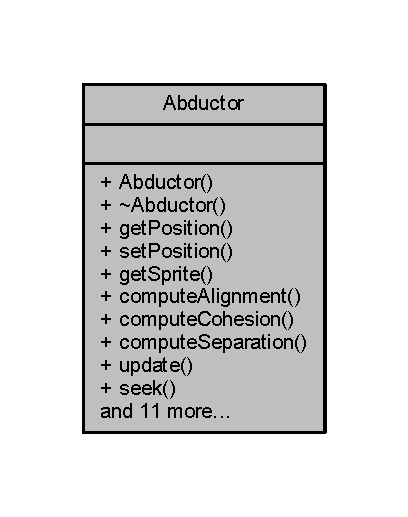
\includegraphics[width=196pt]{class_abductor__coll__graph}
\end{center}
\end{figure}
\subsection*{Public Member Functions}
\begin{DoxyCompactItemize}
\item 
\hyperlink{class_abductor_a2b772afe64f564d1616f2513dfdb7d3e}{Abductor} (sf\+::\+Vector2f \+\_\+pos, sf\+::\+Vector2f \+\_\+vel, sf\+::\+Texture \+\_\+tex, sf\+::\+Texture \+\_\+bullet\+Texture)
\item 
\hyperlink{class_abductor_adc657b211a1b36c55db079caa10d9010}{$\sim$\+Abductor} ()
\item 
sf\+::\+Vector2f \hyperlink{class_abductor_a05b0a89323473488328dafa939e7252a}{get\+Position} ()
\item 
void \hyperlink{class_abductor_a8120f5a1284a3269345b213dc1074d17}{set\+Position} (sf\+::\+Vector2f \+\_\+temp\+Pos)
\item 
sf\+::\+Sprite \hyperlink{class_abductor_a604e41fd9403b542c83859027e8c67d4}{get\+Sprite} ()
\item 
sf\+::\+Vector2f \hyperlink{class_abductor_a1a22ca1f62b22a3e6ab183c0d07215c9}{compute\+Alignment} (std\+::vector$<$ \hyperlink{class_abductor}{Abductor} $\ast$$>$ agents)
\item 
sf\+::\+Vector2f \hyperlink{class_abductor_a8aa45d9b7d770533a60eae180c08d96f}{compute\+Cohesion} (std\+::vector$<$ \hyperlink{class_abductor}{Abductor} $\ast$$>$ agents)
\item 
sf\+::\+Vector2f \hyperlink{class_abductor_ac72ef77b379beff56efed7f66442c649}{compute\+Separation} (std\+::vector$<$ \hyperlink{class_abductor}{Abductor} $\ast$$>$ agents)
\item 
void \hyperlink{class_abductor_a1e3842b4fc70f8667b0e30f23bbce579}{update} ()
\item 
void \hyperlink{class_abductor_a6562333549ea4d8ef5d389e0594de7c1}{seek} (sf\+::\+Vector2f target\+Pos)
\item 
sf\+::\+Vector2f \hyperlink{class_abductor_a98f8c01f0131c30842121b0916fe89b2}{Normalise} (sf\+::\+Vector2f velocity)
\item 
void \hyperlink{class_abductor_a378997aa8cccf0b840f9ef8ba2970699}{movement} (sf\+::\+Vector2f \+\_\+player\+Pos)
\item 
void \hyperlink{class_abductor_a10a4ded56dcad749b1a1656688d135ea}{wander} (std\+::vector$<$ \hyperlink{class_abductor}{Abductor} $\ast$$>$ agents)
\item 
void \hyperlink{class_abductor_aa790b94b30a6bee13c26ffa4b093af6a}{abducting} ()
\item 
void \hyperlink{class_abductor_a1069f5de8e0696be938a741f4b931855}{set\+Abducting} (bool value)
\item 
int \hyperlink{class_abductor_a6893de5e10abe1978bfae651751f2a33}{get\+Health} ()
\item 
void \hyperlink{class_abductor_aa7086d22f21d43097e7d51dd06b4b074}{take\+Damage} (int value)
\item 
sf\+::\+Vector2f \hyperlink{class_abductor_a1f26bdb461e53aa966d744100568d90c}{get\+Velocity} ()
\item 
void \hyperlink{class_abductor_a4eab3b0823078780f2129873bcd181ae}{set\+Index} (int value)
\item 
std\+::vector$<$ \hyperlink{class_bullet}{Bullet} $\ast$ $>$ \& \hyperlink{class_abductor_ac9a6ed96e2b0ffce0984656f8cff114e}{get\+Bullets} ()
\item 
sf\+::\+Rectangle\+Shape \hyperlink{class_abductor_a52e15ddbcabbe719425cdaf98c02b079}{get\+Collision\+Rect} ()
\end{DoxyCompactItemize}


\subsection{Constructor \& Destructor Documentation}
\mbox{\Hypertarget{class_abductor_a2b772afe64f564d1616f2513dfdb7d3e}\label{class_abductor_a2b772afe64f564d1616f2513dfdb7d3e}} 
\index{Abductor@{Abductor}!Abductor@{Abductor}}
\index{Abductor@{Abductor}!Abductor@{Abductor}}
\subsubsection{\texorpdfstring{Abductor()}{Abductor()}}
{\footnotesize\ttfamily Abductor\+::\+Abductor (\begin{DoxyParamCaption}\item[{sf\+::\+Vector2f}]{\+\_\+pos,  }\item[{sf\+::\+Vector2f}]{\+\_\+vel,  }\item[{sf\+::\+Texture}]{\+\_\+tex,  }\item[{sf\+::\+Texture}]{\+\_\+bullet\+Texture }\end{DoxyParamCaption})}

\mbox{\Hypertarget{class_abductor_adc657b211a1b36c55db079caa10d9010}\label{class_abductor_adc657b211a1b36c55db079caa10d9010}} 
\index{Abductor@{Abductor}!````~Abductor@{$\sim$\+Abductor}}
\index{````~Abductor@{$\sim$\+Abductor}!Abductor@{Abductor}}
\subsubsection{\texorpdfstring{$\sim$\+Abductor()}{~Abductor()}}
{\footnotesize\ttfamily Abductor\+::$\sim$\+Abductor (\begin{DoxyParamCaption}{ }\end{DoxyParamCaption})}



\subsection{Member Function Documentation}
\mbox{\Hypertarget{class_abductor_aa790b94b30a6bee13c26ffa4b093af6a}\label{class_abductor_aa790b94b30a6bee13c26ffa4b093af6a}} 
\index{Abductor@{Abductor}!abducting@{abducting}}
\index{abducting@{abducting}!Abductor@{Abductor}}
\subsubsection{\texorpdfstring{abducting()}{abducting()}}
{\footnotesize\ttfamily void Abductor\+::abducting (\begin{DoxyParamCaption}{ }\end{DoxyParamCaption})}

\mbox{\Hypertarget{class_abductor_a1a22ca1f62b22a3e6ab183c0d07215c9}\label{class_abductor_a1a22ca1f62b22a3e6ab183c0d07215c9}} 
\index{Abductor@{Abductor}!compute\+Alignment@{compute\+Alignment}}
\index{compute\+Alignment@{compute\+Alignment}!Abductor@{Abductor}}
\subsubsection{\texorpdfstring{compute\+Alignment()}{computeAlignment()}}
{\footnotesize\ttfamily sf\+::\+Vector2f Abductor\+::compute\+Alignment (\begin{DoxyParamCaption}\item[{std\+::vector$<$ \hyperlink{class_abductor}{Abductor} $\ast$$>$}]{agents }\end{DoxyParamCaption})}

Here is the call graph for this function\+:
\nopagebreak
\begin{figure}[H]
\begin{center}
\leavevmode
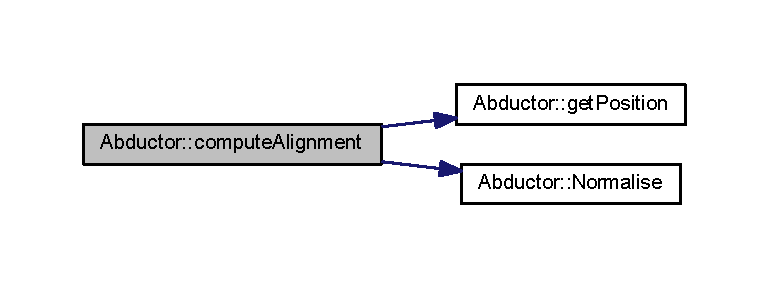
\includegraphics[width=350pt]{class_abductor_a1a22ca1f62b22a3e6ab183c0d07215c9_cgraph}
\end{center}
\end{figure}
\mbox{\Hypertarget{class_abductor_a8aa45d9b7d770533a60eae180c08d96f}\label{class_abductor_a8aa45d9b7d770533a60eae180c08d96f}} 
\index{Abductor@{Abductor}!compute\+Cohesion@{compute\+Cohesion}}
\index{compute\+Cohesion@{compute\+Cohesion}!Abductor@{Abductor}}
\subsubsection{\texorpdfstring{compute\+Cohesion()}{computeCohesion()}}
{\footnotesize\ttfamily sf\+::\+Vector2f Abductor\+::compute\+Cohesion (\begin{DoxyParamCaption}\item[{std\+::vector$<$ \hyperlink{class_abductor}{Abductor} $\ast$$>$}]{agents }\end{DoxyParamCaption})}

Here is the call graph for this function\+:
\nopagebreak
\begin{figure}[H]
\begin{center}
\leavevmode
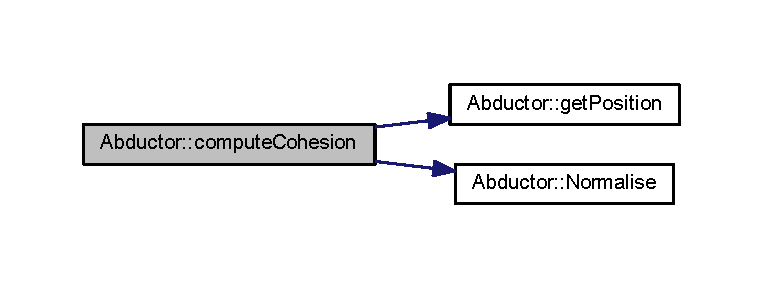
\includegraphics[width=350pt]{class_abductor_a8aa45d9b7d770533a60eae180c08d96f_cgraph}
\end{center}
\end{figure}
\mbox{\Hypertarget{class_abductor_ac72ef77b379beff56efed7f66442c649}\label{class_abductor_ac72ef77b379beff56efed7f66442c649}} 
\index{Abductor@{Abductor}!compute\+Separation@{compute\+Separation}}
\index{compute\+Separation@{compute\+Separation}!Abductor@{Abductor}}
\subsubsection{\texorpdfstring{compute\+Separation()}{computeSeparation()}}
{\footnotesize\ttfamily sf\+::\+Vector2f Abductor\+::compute\+Separation (\begin{DoxyParamCaption}\item[{std\+::vector$<$ \hyperlink{class_abductor}{Abductor} $\ast$$>$}]{agents }\end{DoxyParamCaption})}

Here is the call graph for this function\+:
\nopagebreak
\begin{figure}[H]
\begin{center}
\leavevmode
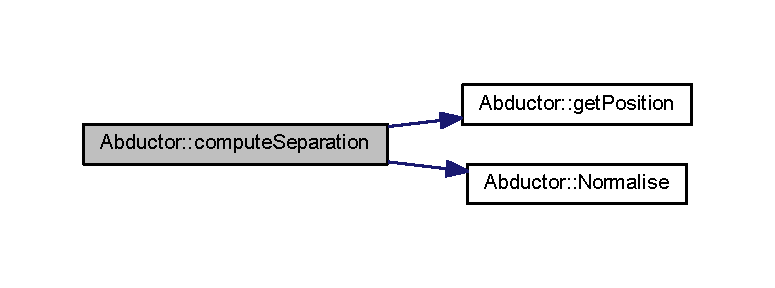
\includegraphics[width=350pt]{class_abductor_ac72ef77b379beff56efed7f66442c649_cgraph}
\end{center}
\end{figure}
\mbox{\Hypertarget{class_abductor_ac9a6ed96e2b0ffce0984656f8cff114e}\label{class_abductor_ac9a6ed96e2b0ffce0984656f8cff114e}} 
\index{Abductor@{Abductor}!get\+Bullets@{get\+Bullets}}
\index{get\+Bullets@{get\+Bullets}!Abductor@{Abductor}}
\subsubsection{\texorpdfstring{get\+Bullets()}{getBullets()}}
{\footnotesize\ttfamily std\+::vector$<$ \hyperlink{class_bullet}{Bullet} $\ast$ $>$ \& Abductor\+::get\+Bullets (\begin{DoxyParamCaption}{ }\end{DoxyParamCaption})}

\mbox{\Hypertarget{class_abductor_a52e15ddbcabbe719425cdaf98c02b079}\label{class_abductor_a52e15ddbcabbe719425cdaf98c02b079}} 
\index{Abductor@{Abductor}!get\+Collision\+Rect@{get\+Collision\+Rect}}
\index{get\+Collision\+Rect@{get\+Collision\+Rect}!Abductor@{Abductor}}
\subsubsection{\texorpdfstring{get\+Collision\+Rect()}{getCollisionRect()}}
{\footnotesize\ttfamily sf\+::\+Rectangle\+Shape Abductor\+::get\+Collision\+Rect (\begin{DoxyParamCaption}{ }\end{DoxyParamCaption})}

\mbox{\Hypertarget{class_abductor_a6893de5e10abe1978bfae651751f2a33}\label{class_abductor_a6893de5e10abe1978bfae651751f2a33}} 
\index{Abductor@{Abductor}!get\+Health@{get\+Health}}
\index{get\+Health@{get\+Health}!Abductor@{Abductor}}
\subsubsection{\texorpdfstring{get\+Health()}{getHealth()}}
{\footnotesize\ttfamily int Abductor\+::get\+Health (\begin{DoxyParamCaption}{ }\end{DoxyParamCaption})}

\mbox{\Hypertarget{class_abductor_a05b0a89323473488328dafa939e7252a}\label{class_abductor_a05b0a89323473488328dafa939e7252a}} 
\index{Abductor@{Abductor}!get\+Position@{get\+Position}}
\index{get\+Position@{get\+Position}!Abductor@{Abductor}}
\subsubsection{\texorpdfstring{get\+Position()}{getPosition()}}
{\footnotesize\ttfamily sf\+::\+Vector2f Abductor\+::get\+Position (\begin{DoxyParamCaption}{ }\end{DoxyParamCaption})}

Here is the caller graph for this function\+:
\nopagebreak
\begin{figure}[H]
\begin{center}
\leavevmode
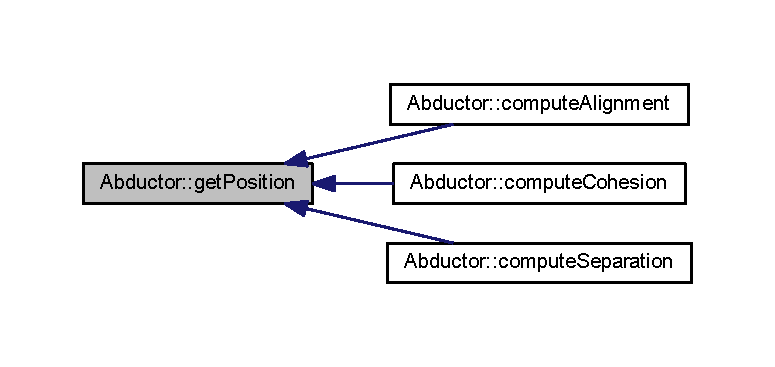
\includegraphics[width=350pt]{class_abductor_a05b0a89323473488328dafa939e7252a_icgraph}
\end{center}
\end{figure}
\mbox{\Hypertarget{class_abductor_a604e41fd9403b542c83859027e8c67d4}\label{class_abductor_a604e41fd9403b542c83859027e8c67d4}} 
\index{Abductor@{Abductor}!get\+Sprite@{get\+Sprite}}
\index{get\+Sprite@{get\+Sprite}!Abductor@{Abductor}}
\subsubsection{\texorpdfstring{get\+Sprite()}{getSprite()}}
{\footnotesize\ttfamily sf\+::\+Sprite Abductor\+::get\+Sprite (\begin{DoxyParamCaption}{ }\end{DoxyParamCaption})}

\mbox{\Hypertarget{class_abductor_a1f26bdb461e53aa966d744100568d90c}\label{class_abductor_a1f26bdb461e53aa966d744100568d90c}} 
\index{Abductor@{Abductor}!get\+Velocity@{get\+Velocity}}
\index{get\+Velocity@{get\+Velocity}!Abductor@{Abductor}}
\subsubsection{\texorpdfstring{get\+Velocity()}{getVelocity()}}
{\footnotesize\ttfamily sf\+::\+Vector2f Abductor\+::get\+Velocity (\begin{DoxyParamCaption}{ }\end{DoxyParamCaption})}

\mbox{\Hypertarget{class_abductor_a378997aa8cccf0b840f9ef8ba2970699}\label{class_abductor_a378997aa8cccf0b840f9ef8ba2970699}} 
\index{Abductor@{Abductor}!movement@{movement}}
\index{movement@{movement}!Abductor@{Abductor}}
\subsubsection{\texorpdfstring{movement()}{movement()}}
{\footnotesize\ttfamily void Abductor\+::movement (\begin{DoxyParamCaption}\item[{sf\+::\+Vector2f}]{\+\_\+player\+Pos }\end{DoxyParamCaption})}

\mbox{\Hypertarget{class_abductor_a98f8c01f0131c30842121b0916fe89b2}\label{class_abductor_a98f8c01f0131c30842121b0916fe89b2}} 
\index{Abductor@{Abductor}!Normalise@{Normalise}}
\index{Normalise@{Normalise}!Abductor@{Abductor}}
\subsubsection{\texorpdfstring{Normalise()}{Normalise()}}
{\footnotesize\ttfamily sf\+::\+Vector2f Abductor\+::\+Normalise (\begin{DoxyParamCaption}\item[{sf\+::\+Vector2f}]{velocity }\end{DoxyParamCaption})}

Here is the caller graph for this function\+:
\nopagebreak
\begin{figure}[H]
\begin{center}
\leavevmode
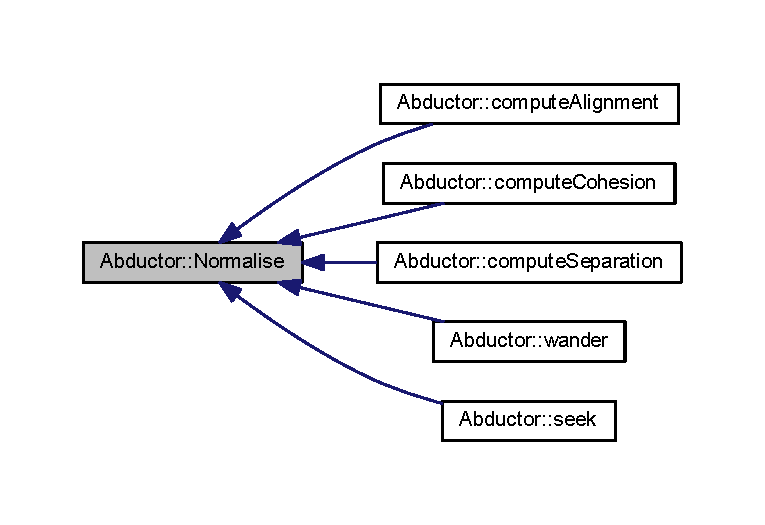
\includegraphics[width=350pt]{class_abductor_a98f8c01f0131c30842121b0916fe89b2_icgraph}
\end{center}
\end{figure}
\mbox{\Hypertarget{class_abductor_a6562333549ea4d8ef5d389e0594de7c1}\label{class_abductor_a6562333549ea4d8ef5d389e0594de7c1}} 
\index{Abductor@{Abductor}!seek@{seek}}
\index{seek@{seek}!Abductor@{Abductor}}
\subsubsection{\texorpdfstring{seek()}{seek()}}
{\footnotesize\ttfamily void Abductor\+::seek (\begin{DoxyParamCaption}\item[{sf\+::\+Vector2f}]{target\+Pos }\end{DoxyParamCaption})}

Here is the call graph for this function\+:
\nopagebreak
\begin{figure}[H]
\begin{center}
\leavevmode
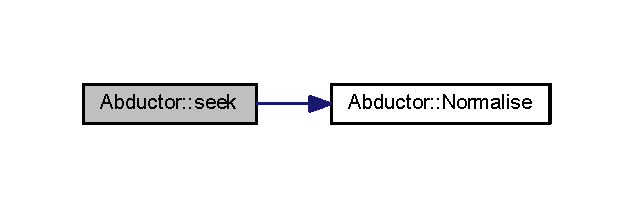
\includegraphics[width=304pt]{class_abductor_a6562333549ea4d8ef5d389e0594de7c1_cgraph}
\end{center}
\end{figure}
\mbox{\Hypertarget{class_abductor_a1069f5de8e0696be938a741f4b931855}\label{class_abductor_a1069f5de8e0696be938a741f4b931855}} 
\index{Abductor@{Abductor}!set\+Abducting@{set\+Abducting}}
\index{set\+Abducting@{set\+Abducting}!Abductor@{Abductor}}
\subsubsection{\texorpdfstring{set\+Abducting()}{setAbducting()}}
{\footnotesize\ttfamily void Abductor\+::set\+Abducting (\begin{DoxyParamCaption}\item[{bool}]{value }\end{DoxyParamCaption})}

\mbox{\Hypertarget{class_abductor_a4eab3b0823078780f2129873bcd181ae}\label{class_abductor_a4eab3b0823078780f2129873bcd181ae}} 
\index{Abductor@{Abductor}!set\+Index@{set\+Index}}
\index{set\+Index@{set\+Index}!Abductor@{Abductor}}
\subsubsection{\texorpdfstring{set\+Index()}{setIndex()}}
{\footnotesize\ttfamily void Abductor\+::set\+Index (\begin{DoxyParamCaption}\item[{int}]{value }\end{DoxyParamCaption})}

\mbox{\Hypertarget{class_abductor_a8120f5a1284a3269345b213dc1074d17}\label{class_abductor_a8120f5a1284a3269345b213dc1074d17}} 
\index{Abductor@{Abductor}!set\+Position@{set\+Position}}
\index{set\+Position@{set\+Position}!Abductor@{Abductor}}
\subsubsection{\texorpdfstring{set\+Position()}{setPosition()}}
{\footnotesize\ttfamily void Abductor\+::set\+Position (\begin{DoxyParamCaption}\item[{sf\+::\+Vector2f}]{\+\_\+temp\+Pos }\end{DoxyParamCaption})}

\mbox{\Hypertarget{class_abductor_aa7086d22f21d43097e7d51dd06b4b074}\label{class_abductor_aa7086d22f21d43097e7d51dd06b4b074}} 
\index{Abductor@{Abductor}!take\+Damage@{take\+Damage}}
\index{take\+Damage@{take\+Damage}!Abductor@{Abductor}}
\subsubsection{\texorpdfstring{take\+Damage()}{takeDamage()}}
{\footnotesize\ttfamily void Abductor\+::take\+Damage (\begin{DoxyParamCaption}\item[{int}]{value }\end{DoxyParamCaption})}

\mbox{\Hypertarget{class_abductor_a1e3842b4fc70f8667b0e30f23bbce579}\label{class_abductor_a1e3842b4fc70f8667b0e30f23bbce579}} 
\index{Abductor@{Abductor}!update@{update}}
\index{update@{update}!Abductor@{Abductor}}
\subsubsection{\texorpdfstring{update()}{update()}}
{\footnotesize\ttfamily void Abductor\+::update (\begin{DoxyParamCaption}{ }\end{DoxyParamCaption})}

\mbox{\Hypertarget{class_abductor_a10a4ded56dcad749b1a1656688d135ea}\label{class_abductor_a10a4ded56dcad749b1a1656688d135ea}} 
\index{Abductor@{Abductor}!wander@{wander}}
\index{wander@{wander}!Abductor@{Abductor}}
\subsubsection{\texorpdfstring{wander()}{wander()}}
{\footnotesize\ttfamily void Abductor\+::wander (\begin{DoxyParamCaption}\item[{std\+::vector$<$ \hyperlink{class_abductor}{Abductor} $\ast$$>$}]{agents }\end{DoxyParamCaption})}

Here is the call graph for this function\+:
\nopagebreak
\begin{figure}[H]
\begin{center}
\leavevmode
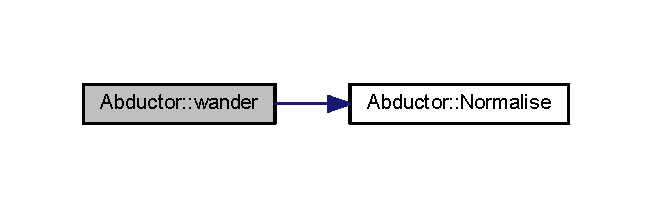
\includegraphics[width=313pt]{class_abductor_a10a4ded56dcad749b1a1656688d135ea_cgraph}
\end{center}
\end{figure}


The documentation for this class was generated from the following files\+:\begin{DoxyCompactItemize}
\item 
\hyperlink{_abductor_8h}{Abductor.\+h}\item 
\hyperlink{_abductor_8cpp}{Abductor.\+cpp}\end{DoxyCompactItemize}

\hypertarget{class_alien_nest}{}\section{Alien\+Nest Class Reference}
\label{class_alien_nest}\index{Alien\+Nest@{Alien\+Nest}}


{\ttfamily \#include $<$Alien\+Nest.\+h$>$}



Collaboration diagram for Alien\+Nest\+:
\nopagebreak
\begin{figure}[H]
\begin{center}
\leavevmode
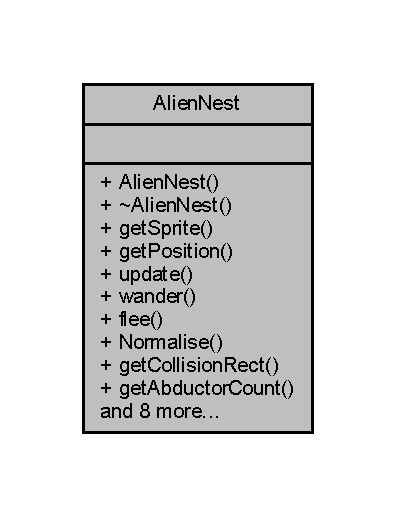
\includegraphics[width=190pt]{class_alien_nest__coll__graph}
\end{center}
\end{figure}
\subsection*{Public Member Functions}
\begin{DoxyCompactItemize}
\item 
\hyperlink{class_alien_nest_ae5468acc196e21772de57cc786bc8922}{Alien\+Nest} (sf\+::\+Vector2f \+\_\+\+Pos, sf\+::\+Vector2f \+\_\+\+Vel, sf\+::\+Texture \+\_\+\+Tex)
\item 
\hyperlink{class_alien_nest_adf76d39d4b159b48b685e28b48e65af4}{$\sim$\+Alien\+Nest} ()
\item 
sf\+::\+Sprite \hyperlink{class_alien_nest_ab37d12dc080c9433d0b34324160c4540}{get\+Sprite} ()
\item 
sf\+::\+Vector2f \hyperlink{class_alien_nest_a1d0491e4d757b1f068fcdfdff3af4263}{get\+Position} ()
\item 
void \hyperlink{class_alien_nest_a4dc29eea96da989af765ac1c0b92cbe0}{update} (sf\+::\+Vector2f player\+Pos, sf\+::\+Texture \+\_\+alien\+Missile)
\item 
void \hyperlink{class_alien_nest_ac2679698409238879ace3367ceba6d9d}{wander} ()
\item 
void \hyperlink{class_alien_nest_a79b79e01b2c2c191a62f6522e62e7093}{flee} (sf\+::\+Vector2f player\+Pos)
\item 
sf\+::\+Vector2f \hyperlink{class_alien_nest_a1482a4dc78827c14dd442a8d9a0a36e3}{Normalise} (sf\+::\+Vector2f velocity)
\item 
sf\+::\+Rectangle\+Shape \hyperlink{class_alien_nest_a7522ad4ae88e2471de29ab62451ec36a}{get\+Collision\+Rect} ()
\item 
int \hyperlink{class_alien_nest_ac5004adc73493a1f3f0807cd03b522c8}{get\+Abductor\+Count} ()
\item 
void \hyperlink{class_alien_nest_a0b47d6d12801e07c6d59592d37444c81}{set\+Abductor\+Count} (int value)
\item 
int \hyperlink{class_alien_nest_a076132ab9da2dae0b0a4eb66b7dc41b8}{get\+Bullet\+Count} ()
\item 
void \hyperlink{class_alien_nest_a050a64974389f5f6d4fbd1c74aa30bb5}{set\+Bullet\+Count} (int value)
\item 
int \hyperlink{class_alien_nest_ad8eb2e360b956e44ec9da1d0da42cf88}{get\+Abductor\+Spawn\+Timer} ()
\item 
void \hyperlink{class_alien_nest_ac19100b42e3fda84431a918517411573}{set\+Abductor\+Spawn\+Timer} (int value)
\item 
int \hyperlink{class_alien_nest_adca5cfd4eae3e3f72dd76960a29588e9}{get\+Health} ()
\item 
void \hyperlink{class_alien_nest_a49b484cdb9ba5c49e1d2912f359b66c5}{take\+Damage} (int value)
\item 
std\+::vector$<$ \hyperlink{class_bullet}{Bullet} $\ast$ $>$ \& \hyperlink{class_alien_nest_a06b510eab5f7bb869078662f42080738}{get\+Bullets} ()
\end{DoxyCompactItemize}


\subsection{Constructor \& Destructor Documentation}
\mbox{\Hypertarget{class_alien_nest_ae5468acc196e21772de57cc786bc8922}\label{class_alien_nest_ae5468acc196e21772de57cc786bc8922}} 
\index{Alien\+Nest@{Alien\+Nest}!Alien\+Nest@{Alien\+Nest}}
\index{Alien\+Nest@{Alien\+Nest}!Alien\+Nest@{Alien\+Nest}}
\subsubsection{\texorpdfstring{Alien\+Nest()}{AlienNest()}}
{\footnotesize\ttfamily Alien\+Nest\+::\+Alien\+Nest (\begin{DoxyParamCaption}\item[{sf\+::\+Vector2f}]{\+\_\+\+Pos,  }\item[{sf\+::\+Vector2f}]{\+\_\+\+Vel,  }\item[{sf\+::\+Texture}]{\+\_\+\+Tex }\end{DoxyParamCaption})}

\mbox{\Hypertarget{class_alien_nest_adf76d39d4b159b48b685e28b48e65af4}\label{class_alien_nest_adf76d39d4b159b48b685e28b48e65af4}} 
\index{Alien\+Nest@{Alien\+Nest}!````~Alien\+Nest@{$\sim$\+Alien\+Nest}}
\index{````~Alien\+Nest@{$\sim$\+Alien\+Nest}!Alien\+Nest@{Alien\+Nest}}
\subsubsection{\texorpdfstring{$\sim$\+Alien\+Nest()}{~AlienNest()}}
{\footnotesize\ttfamily Alien\+Nest\+::$\sim$\+Alien\+Nest (\begin{DoxyParamCaption}{ }\end{DoxyParamCaption})}



\subsection{Member Function Documentation}
\mbox{\Hypertarget{class_alien_nest_a79b79e01b2c2c191a62f6522e62e7093}\label{class_alien_nest_a79b79e01b2c2c191a62f6522e62e7093}} 
\index{Alien\+Nest@{Alien\+Nest}!flee@{flee}}
\index{flee@{flee}!Alien\+Nest@{Alien\+Nest}}
\subsubsection{\texorpdfstring{flee()}{flee()}}
{\footnotesize\ttfamily void Alien\+Nest\+::flee (\begin{DoxyParamCaption}\item[{sf\+::\+Vector2f}]{player\+Pos }\end{DoxyParamCaption})}

Here is the call graph for this function\+:
\nopagebreak
\begin{figure}[H]
\begin{center}
\leavevmode
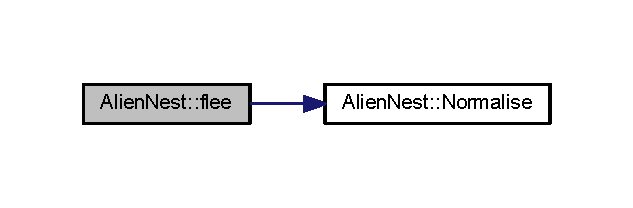
\includegraphics[width=304pt]{class_alien_nest_a79b79e01b2c2c191a62f6522e62e7093_cgraph}
\end{center}
\end{figure}
Here is the caller graph for this function\+:
\nopagebreak
\begin{figure}[H]
\begin{center}
\leavevmode
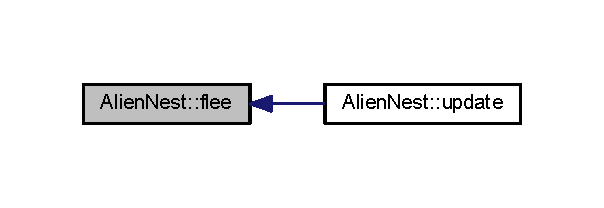
\includegraphics[width=290pt]{class_alien_nest_a79b79e01b2c2c191a62f6522e62e7093_icgraph}
\end{center}
\end{figure}
\mbox{\Hypertarget{class_alien_nest_ac5004adc73493a1f3f0807cd03b522c8}\label{class_alien_nest_ac5004adc73493a1f3f0807cd03b522c8}} 
\index{Alien\+Nest@{Alien\+Nest}!get\+Abductor\+Count@{get\+Abductor\+Count}}
\index{get\+Abductor\+Count@{get\+Abductor\+Count}!Alien\+Nest@{Alien\+Nest}}
\subsubsection{\texorpdfstring{get\+Abductor\+Count()}{getAbductorCount()}}
{\footnotesize\ttfamily int Alien\+Nest\+::get\+Abductor\+Count (\begin{DoxyParamCaption}{ }\end{DoxyParamCaption})}

\mbox{\Hypertarget{class_alien_nest_ad8eb2e360b956e44ec9da1d0da42cf88}\label{class_alien_nest_ad8eb2e360b956e44ec9da1d0da42cf88}} 
\index{Alien\+Nest@{Alien\+Nest}!get\+Abductor\+Spawn\+Timer@{get\+Abductor\+Spawn\+Timer}}
\index{get\+Abductor\+Spawn\+Timer@{get\+Abductor\+Spawn\+Timer}!Alien\+Nest@{Alien\+Nest}}
\subsubsection{\texorpdfstring{get\+Abductor\+Spawn\+Timer()}{getAbductorSpawnTimer()}}
{\footnotesize\ttfamily int Alien\+Nest\+::get\+Abductor\+Spawn\+Timer (\begin{DoxyParamCaption}{ }\end{DoxyParamCaption})}

\mbox{\Hypertarget{class_alien_nest_a076132ab9da2dae0b0a4eb66b7dc41b8}\label{class_alien_nest_a076132ab9da2dae0b0a4eb66b7dc41b8}} 
\index{Alien\+Nest@{Alien\+Nest}!get\+Bullet\+Count@{get\+Bullet\+Count}}
\index{get\+Bullet\+Count@{get\+Bullet\+Count}!Alien\+Nest@{Alien\+Nest}}
\subsubsection{\texorpdfstring{get\+Bullet\+Count()}{getBulletCount()}}
{\footnotesize\ttfamily int Alien\+Nest\+::get\+Bullet\+Count (\begin{DoxyParamCaption}{ }\end{DoxyParamCaption})}

\mbox{\Hypertarget{class_alien_nest_a06b510eab5f7bb869078662f42080738}\label{class_alien_nest_a06b510eab5f7bb869078662f42080738}} 
\index{Alien\+Nest@{Alien\+Nest}!get\+Bullets@{get\+Bullets}}
\index{get\+Bullets@{get\+Bullets}!Alien\+Nest@{Alien\+Nest}}
\subsubsection{\texorpdfstring{get\+Bullets()}{getBullets()}}
{\footnotesize\ttfamily std\+::vector$<$ \hyperlink{class_bullet}{Bullet} $\ast$ $>$ \& Alien\+Nest\+::get\+Bullets (\begin{DoxyParamCaption}{ }\end{DoxyParamCaption})}

\mbox{\Hypertarget{class_alien_nest_a7522ad4ae88e2471de29ab62451ec36a}\label{class_alien_nest_a7522ad4ae88e2471de29ab62451ec36a}} 
\index{Alien\+Nest@{Alien\+Nest}!get\+Collision\+Rect@{get\+Collision\+Rect}}
\index{get\+Collision\+Rect@{get\+Collision\+Rect}!Alien\+Nest@{Alien\+Nest}}
\subsubsection{\texorpdfstring{get\+Collision\+Rect()}{getCollisionRect()}}
{\footnotesize\ttfamily sf\+::\+Rectangle\+Shape Alien\+Nest\+::get\+Collision\+Rect (\begin{DoxyParamCaption}{ }\end{DoxyParamCaption})}

\mbox{\Hypertarget{class_alien_nest_adca5cfd4eae3e3f72dd76960a29588e9}\label{class_alien_nest_adca5cfd4eae3e3f72dd76960a29588e9}} 
\index{Alien\+Nest@{Alien\+Nest}!get\+Health@{get\+Health}}
\index{get\+Health@{get\+Health}!Alien\+Nest@{Alien\+Nest}}
\subsubsection{\texorpdfstring{get\+Health()}{getHealth()}}
{\footnotesize\ttfamily int Alien\+Nest\+::get\+Health (\begin{DoxyParamCaption}{ }\end{DoxyParamCaption})}

\mbox{\Hypertarget{class_alien_nest_a1d0491e4d757b1f068fcdfdff3af4263}\label{class_alien_nest_a1d0491e4d757b1f068fcdfdff3af4263}} 
\index{Alien\+Nest@{Alien\+Nest}!get\+Position@{get\+Position}}
\index{get\+Position@{get\+Position}!Alien\+Nest@{Alien\+Nest}}
\subsubsection{\texorpdfstring{get\+Position()}{getPosition()}}
{\footnotesize\ttfamily sf\+::\+Vector2f Alien\+Nest\+::get\+Position (\begin{DoxyParamCaption}{ }\end{DoxyParamCaption})}

\mbox{\Hypertarget{class_alien_nest_ab37d12dc080c9433d0b34324160c4540}\label{class_alien_nest_ab37d12dc080c9433d0b34324160c4540}} 
\index{Alien\+Nest@{Alien\+Nest}!get\+Sprite@{get\+Sprite}}
\index{get\+Sprite@{get\+Sprite}!Alien\+Nest@{Alien\+Nest}}
\subsubsection{\texorpdfstring{get\+Sprite()}{getSprite()}}
{\footnotesize\ttfamily sf\+::\+Sprite Alien\+Nest\+::get\+Sprite (\begin{DoxyParamCaption}{ }\end{DoxyParamCaption})}

\mbox{\Hypertarget{class_alien_nest_a1482a4dc78827c14dd442a8d9a0a36e3}\label{class_alien_nest_a1482a4dc78827c14dd442a8d9a0a36e3}} 
\index{Alien\+Nest@{Alien\+Nest}!Normalise@{Normalise}}
\index{Normalise@{Normalise}!Alien\+Nest@{Alien\+Nest}}
\subsubsection{\texorpdfstring{Normalise()}{Normalise()}}
{\footnotesize\ttfamily sf\+::\+Vector2f Alien\+Nest\+::\+Normalise (\begin{DoxyParamCaption}\item[{sf\+::\+Vector2f}]{velocity }\end{DoxyParamCaption})}

Here is the caller graph for this function\+:
\nopagebreak
\begin{figure}[H]
\begin{center}
\leavevmode
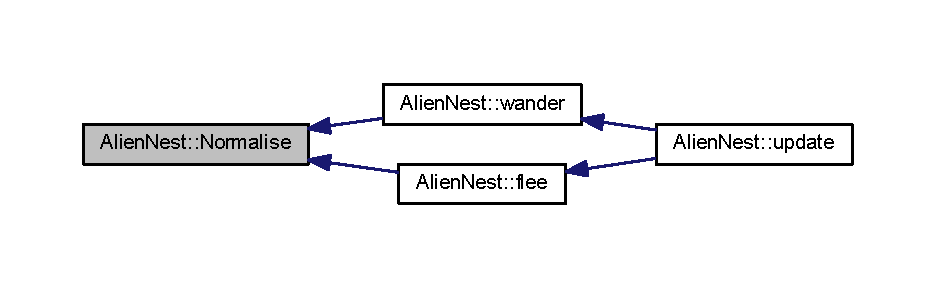
\includegraphics[width=350pt]{class_alien_nest_a1482a4dc78827c14dd442a8d9a0a36e3_icgraph}
\end{center}
\end{figure}
\mbox{\Hypertarget{class_alien_nest_a0b47d6d12801e07c6d59592d37444c81}\label{class_alien_nest_a0b47d6d12801e07c6d59592d37444c81}} 
\index{Alien\+Nest@{Alien\+Nest}!set\+Abductor\+Count@{set\+Abductor\+Count}}
\index{set\+Abductor\+Count@{set\+Abductor\+Count}!Alien\+Nest@{Alien\+Nest}}
\subsubsection{\texorpdfstring{set\+Abductor\+Count()}{setAbductorCount()}}
{\footnotesize\ttfamily void Alien\+Nest\+::set\+Abductor\+Count (\begin{DoxyParamCaption}\item[{int}]{value }\end{DoxyParamCaption})}

\mbox{\Hypertarget{class_alien_nest_ac19100b42e3fda84431a918517411573}\label{class_alien_nest_ac19100b42e3fda84431a918517411573}} 
\index{Alien\+Nest@{Alien\+Nest}!set\+Abductor\+Spawn\+Timer@{set\+Abductor\+Spawn\+Timer}}
\index{set\+Abductor\+Spawn\+Timer@{set\+Abductor\+Spawn\+Timer}!Alien\+Nest@{Alien\+Nest}}
\subsubsection{\texorpdfstring{set\+Abductor\+Spawn\+Timer()}{setAbductorSpawnTimer()}}
{\footnotesize\ttfamily void Alien\+Nest\+::set\+Abductor\+Spawn\+Timer (\begin{DoxyParamCaption}\item[{int}]{value }\end{DoxyParamCaption})}

\mbox{\Hypertarget{class_alien_nest_a050a64974389f5f6d4fbd1c74aa30bb5}\label{class_alien_nest_a050a64974389f5f6d4fbd1c74aa30bb5}} 
\index{Alien\+Nest@{Alien\+Nest}!set\+Bullet\+Count@{set\+Bullet\+Count}}
\index{set\+Bullet\+Count@{set\+Bullet\+Count}!Alien\+Nest@{Alien\+Nest}}
\subsubsection{\texorpdfstring{set\+Bullet\+Count()}{setBulletCount()}}
{\footnotesize\ttfamily void Alien\+Nest\+::set\+Bullet\+Count (\begin{DoxyParamCaption}\item[{int}]{value }\end{DoxyParamCaption})}

\mbox{\Hypertarget{class_alien_nest_a49b484cdb9ba5c49e1d2912f359b66c5}\label{class_alien_nest_a49b484cdb9ba5c49e1d2912f359b66c5}} 
\index{Alien\+Nest@{Alien\+Nest}!take\+Damage@{take\+Damage}}
\index{take\+Damage@{take\+Damage}!Alien\+Nest@{Alien\+Nest}}
\subsubsection{\texorpdfstring{take\+Damage()}{takeDamage()}}
{\footnotesize\ttfamily void Alien\+Nest\+::take\+Damage (\begin{DoxyParamCaption}\item[{int}]{value }\end{DoxyParamCaption})}

\mbox{\Hypertarget{class_alien_nest_a4dc29eea96da989af765ac1c0b92cbe0}\label{class_alien_nest_a4dc29eea96da989af765ac1c0b92cbe0}} 
\index{Alien\+Nest@{Alien\+Nest}!update@{update}}
\index{update@{update}!Alien\+Nest@{Alien\+Nest}}
\subsubsection{\texorpdfstring{update()}{update()}}
{\footnotesize\ttfamily void Alien\+Nest\+::update (\begin{DoxyParamCaption}\item[{sf\+::\+Vector2f}]{player\+Pos,  }\item[{sf\+::\+Texture}]{\+\_\+alien\+Missile }\end{DoxyParamCaption})}

Here is the call graph for this function\+:
\nopagebreak
\begin{figure}[H]
\begin{center}
\leavevmode
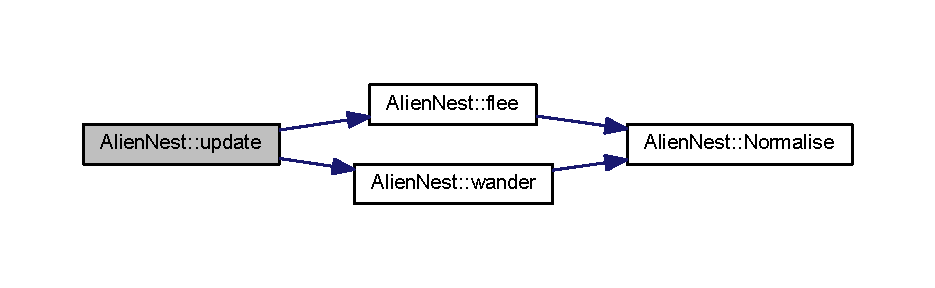
\includegraphics[width=350pt]{class_alien_nest_a4dc29eea96da989af765ac1c0b92cbe0_cgraph}
\end{center}
\end{figure}
\mbox{\Hypertarget{class_alien_nest_ac2679698409238879ace3367ceba6d9d}\label{class_alien_nest_ac2679698409238879ace3367ceba6d9d}} 
\index{Alien\+Nest@{Alien\+Nest}!wander@{wander}}
\index{wander@{wander}!Alien\+Nest@{Alien\+Nest}}
\subsubsection{\texorpdfstring{wander()}{wander()}}
{\footnotesize\ttfamily void Alien\+Nest\+::wander (\begin{DoxyParamCaption}{ }\end{DoxyParamCaption})}

Here is the call graph for this function\+:
\nopagebreak
\begin{figure}[H]
\begin{center}
\leavevmode
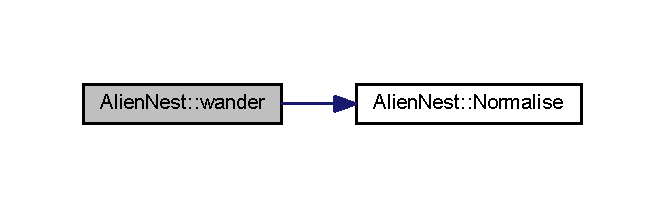
\includegraphics[width=319pt]{class_alien_nest_ac2679698409238879ace3367ceba6d9d_cgraph}
\end{center}
\end{figure}
Here is the caller graph for this function\+:
\nopagebreak
\begin{figure}[H]
\begin{center}
\leavevmode
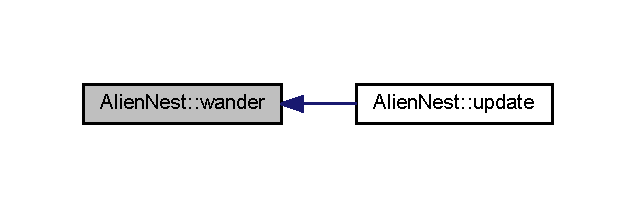
\includegraphics[width=305pt]{class_alien_nest_ac2679698409238879ace3367ceba6d9d_icgraph}
\end{center}
\end{figure}


The documentation for this class was generated from the following files\+:\begin{DoxyCompactItemize}
\item 
\hyperlink{_alien_nest_8h}{Alien\+Nest.\+h}\item 
\hyperlink{_alien_nest_8cpp}{Alien\+Nest.\+cpp}\end{DoxyCompactItemize}

\hypertarget{class_astronaut}{}\section{Astronaut Class Reference}
\label{class_astronaut}\index{Astronaut@{Astronaut}}


{\ttfamily \#include $<$Astronaut.\+h$>$}



Collaboration diagram for Astronaut\+:
\nopagebreak
\begin{figure}[H]
\begin{center}
\leavevmode
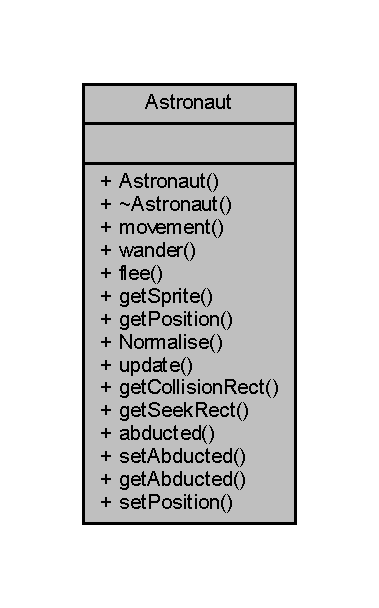
\includegraphics[width=182pt]{class_astronaut__coll__graph}
\end{center}
\end{figure}
\subsection*{Public Member Functions}
\begin{DoxyCompactItemize}
\item 
\hyperlink{class_astronaut_ad88a1f14ffa4e13ebc9d996a7def9c74}{Astronaut} (sf\+::\+Vector2f \+\_\+\+Pos, sf\+::\+Vector2f \+\_\+\+Vel, sf\+::\+Texture \+\_\+\+Tex)
\item 
\hyperlink{class_astronaut_af31f9de205719a042df5f0a1879ee064}{$\sim$\+Astronaut} ()
\item 
void \hyperlink{class_astronaut_ab5c332ef51826c5ef2f89fcc72160401}{movement} (sf\+::\+Vector2f abductor\+Pos)
\item 
void \hyperlink{class_astronaut_a39d7e43f8604bf561570e2eb2564a8fa}{wander} ()
\item 
void \hyperlink{class_astronaut_a81199297e80402f219a58a2fff56372c}{flee} (sf\+::\+Vector2f abductor\+Pos)
\item 
sf\+::\+Sprite \hyperlink{class_astronaut_a0fd66ca32a63fde604ddbeadd1a80edc}{get\+Sprite} ()
\item 
sf\+::\+Vector2f \hyperlink{class_astronaut_a3738ff50527c44f089b110ecdb0be2f3}{get\+Position} ()
\item 
sf\+::\+Vector2f \hyperlink{class_astronaut_a9276590bb221f7809f17ebff0a32db36}{Normalise} (sf\+::\+Vector2f velocity)
\item 
void \hyperlink{class_astronaut_acb963c04f91f1cda4aac81f5a51e1f34}{update} ()
\item 
sf\+::\+Rectangle\+Shape \hyperlink{class_astronaut_a5d01978fdd0f00d9adc9769505baa5d5}{get\+Collision\+Rect} ()
\item 
sf\+::\+Rectangle\+Shape \hyperlink{class_astronaut_a59883964bc6a7997885e341918638f80}{get\+Seek\+Rect} ()
\item 
void \hyperlink{class_astronaut_a33359ffc0867f0e6c83a63ed39659848}{abducted} (sf\+::\+Vector2f \+\_\+abductor\+Pos)
\item 
void \hyperlink{class_astronaut_a07d0b1366726e708be3361795a25a1ce}{set\+Abducted} (bool)
\item 
bool \hyperlink{class_astronaut_a531b1ad1af11a0c788a182fa7b71794f}{get\+Abducted} ()
\item 
void \hyperlink{class_astronaut_a2dff61a54b10d5fb38f68d2f63668387}{set\+Position} (sf\+::\+Vector2f)
\end{DoxyCompactItemize}


\subsection{Constructor \& Destructor Documentation}
\mbox{\Hypertarget{class_astronaut_ad88a1f14ffa4e13ebc9d996a7def9c74}\label{class_astronaut_ad88a1f14ffa4e13ebc9d996a7def9c74}} 
\index{Astronaut@{Astronaut}!Astronaut@{Astronaut}}
\index{Astronaut@{Astronaut}!Astronaut@{Astronaut}}
\subsubsection{\texorpdfstring{Astronaut()}{Astronaut()}}
{\footnotesize\ttfamily Astronaut\+::\+Astronaut (\begin{DoxyParamCaption}\item[{sf\+::\+Vector2f}]{\+\_\+\+Pos,  }\item[{sf\+::\+Vector2f}]{\+\_\+\+Vel,  }\item[{sf\+::\+Texture}]{\+\_\+\+Tex }\end{DoxyParamCaption})}

\mbox{\Hypertarget{class_astronaut_af31f9de205719a042df5f0a1879ee064}\label{class_astronaut_af31f9de205719a042df5f0a1879ee064}} 
\index{Astronaut@{Astronaut}!````~Astronaut@{$\sim$\+Astronaut}}
\index{````~Astronaut@{$\sim$\+Astronaut}!Astronaut@{Astronaut}}
\subsubsection{\texorpdfstring{$\sim$\+Astronaut()}{~Astronaut()}}
{\footnotesize\ttfamily Astronaut\+::$\sim$\+Astronaut (\begin{DoxyParamCaption}{ }\end{DoxyParamCaption})}



\subsection{Member Function Documentation}
\mbox{\Hypertarget{class_astronaut_a33359ffc0867f0e6c83a63ed39659848}\label{class_astronaut_a33359ffc0867f0e6c83a63ed39659848}} 
\index{Astronaut@{Astronaut}!abducted@{abducted}}
\index{abducted@{abducted}!Astronaut@{Astronaut}}
\subsubsection{\texorpdfstring{abducted()}{abducted()}}
{\footnotesize\ttfamily void Astronaut\+::abducted (\begin{DoxyParamCaption}\item[{sf\+::\+Vector2f}]{\+\_\+abductor\+Pos }\end{DoxyParamCaption})}

\mbox{\Hypertarget{class_astronaut_a81199297e80402f219a58a2fff56372c}\label{class_astronaut_a81199297e80402f219a58a2fff56372c}} 
\index{Astronaut@{Astronaut}!flee@{flee}}
\index{flee@{flee}!Astronaut@{Astronaut}}
\subsubsection{\texorpdfstring{flee()}{flee()}}
{\footnotesize\ttfamily void Astronaut\+::flee (\begin{DoxyParamCaption}\item[{sf\+::\+Vector2f}]{abductor\+Pos }\end{DoxyParamCaption})}

Here is the call graph for this function\+:
\nopagebreak
\begin{figure}[H]
\begin{center}
\leavevmode
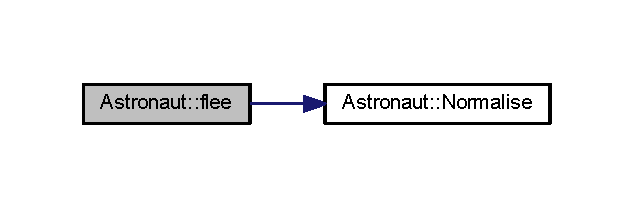
\includegraphics[width=304pt]{class_astronaut_a81199297e80402f219a58a2fff56372c_cgraph}
\end{center}
\end{figure}
Here is the caller graph for this function\+:
\nopagebreak
\begin{figure}[H]
\begin{center}
\leavevmode
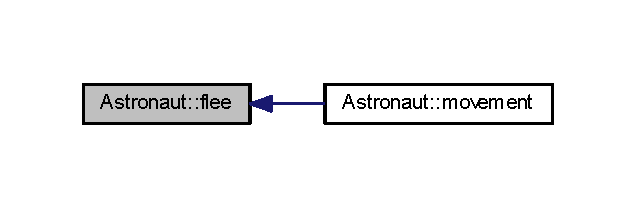
\includegraphics[width=305pt]{class_astronaut_a81199297e80402f219a58a2fff56372c_icgraph}
\end{center}
\end{figure}
\mbox{\Hypertarget{class_astronaut_a531b1ad1af11a0c788a182fa7b71794f}\label{class_astronaut_a531b1ad1af11a0c788a182fa7b71794f}} 
\index{Astronaut@{Astronaut}!get\+Abducted@{get\+Abducted}}
\index{get\+Abducted@{get\+Abducted}!Astronaut@{Astronaut}}
\subsubsection{\texorpdfstring{get\+Abducted()}{getAbducted()}}
{\footnotesize\ttfamily bool Astronaut\+::get\+Abducted (\begin{DoxyParamCaption}{ }\end{DoxyParamCaption})}

\mbox{\Hypertarget{class_astronaut_a5d01978fdd0f00d9adc9769505baa5d5}\label{class_astronaut_a5d01978fdd0f00d9adc9769505baa5d5}} 
\index{Astronaut@{Astronaut}!get\+Collision\+Rect@{get\+Collision\+Rect}}
\index{get\+Collision\+Rect@{get\+Collision\+Rect}!Astronaut@{Astronaut}}
\subsubsection{\texorpdfstring{get\+Collision\+Rect()}{getCollisionRect()}}
{\footnotesize\ttfamily sf\+::\+Rectangle\+Shape Astronaut\+::get\+Collision\+Rect (\begin{DoxyParamCaption}{ }\end{DoxyParamCaption})}

\mbox{\Hypertarget{class_astronaut_a3738ff50527c44f089b110ecdb0be2f3}\label{class_astronaut_a3738ff50527c44f089b110ecdb0be2f3}} 
\index{Astronaut@{Astronaut}!get\+Position@{get\+Position}}
\index{get\+Position@{get\+Position}!Astronaut@{Astronaut}}
\subsubsection{\texorpdfstring{get\+Position()}{getPosition()}}
{\footnotesize\ttfamily sf\+::\+Vector2f Astronaut\+::get\+Position (\begin{DoxyParamCaption}{ }\end{DoxyParamCaption})}

\mbox{\Hypertarget{class_astronaut_a59883964bc6a7997885e341918638f80}\label{class_astronaut_a59883964bc6a7997885e341918638f80}} 
\index{Astronaut@{Astronaut}!get\+Seek\+Rect@{get\+Seek\+Rect}}
\index{get\+Seek\+Rect@{get\+Seek\+Rect}!Astronaut@{Astronaut}}
\subsubsection{\texorpdfstring{get\+Seek\+Rect()}{getSeekRect()}}
{\footnotesize\ttfamily sf\+::\+Rectangle\+Shape Astronaut\+::get\+Seek\+Rect (\begin{DoxyParamCaption}{ }\end{DoxyParamCaption})}

\mbox{\Hypertarget{class_astronaut_a0fd66ca32a63fde604ddbeadd1a80edc}\label{class_astronaut_a0fd66ca32a63fde604ddbeadd1a80edc}} 
\index{Astronaut@{Astronaut}!get\+Sprite@{get\+Sprite}}
\index{get\+Sprite@{get\+Sprite}!Astronaut@{Astronaut}}
\subsubsection{\texorpdfstring{get\+Sprite()}{getSprite()}}
{\footnotesize\ttfamily sf\+::\+Sprite Astronaut\+::get\+Sprite (\begin{DoxyParamCaption}{ }\end{DoxyParamCaption})}

\mbox{\Hypertarget{class_astronaut_ab5c332ef51826c5ef2f89fcc72160401}\label{class_astronaut_ab5c332ef51826c5ef2f89fcc72160401}} 
\index{Astronaut@{Astronaut}!movement@{movement}}
\index{movement@{movement}!Astronaut@{Astronaut}}
\subsubsection{\texorpdfstring{movement()}{movement()}}
{\footnotesize\ttfamily void Astronaut\+::movement (\begin{DoxyParamCaption}\item[{sf\+::\+Vector2f}]{abductor\+Pos }\end{DoxyParamCaption})}

Here is the call graph for this function\+:
\nopagebreak
\begin{figure}[H]
\begin{center}
\leavevmode
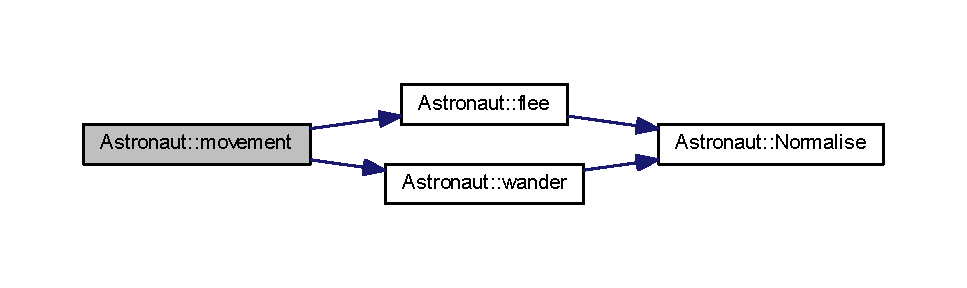
\includegraphics[width=350pt]{class_astronaut_ab5c332ef51826c5ef2f89fcc72160401_cgraph}
\end{center}
\end{figure}
\mbox{\Hypertarget{class_astronaut_a9276590bb221f7809f17ebff0a32db36}\label{class_astronaut_a9276590bb221f7809f17ebff0a32db36}} 
\index{Astronaut@{Astronaut}!Normalise@{Normalise}}
\index{Normalise@{Normalise}!Astronaut@{Astronaut}}
\subsubsection{\texorpdfstring{Normalise()}{Normalise()}}
{\footnotesize\ttfamily sf\+::\+Vector2f Astronaut\+::\+Normalise (\begin{DoxyParamCaption}\item[{sf\+::\+Vector2f}]{velocity }\end{DoxyParamCaption})}

Here is the caller graph for this function\+:
\nopagebreak
\begin{figure}[H]
\begin{center}
\leavevmode
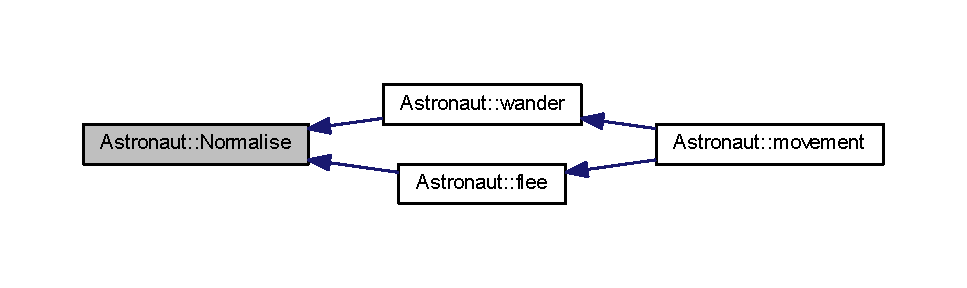
\includegraphics[width=350pt]{class_astronaut_a9276590bb221f7809f17ebff0a32db36_icgraph}
\end{center}
\end{figure}
\mbox{\Hypertarget{class_astronaut_a07d0b1366726e708be3361795a25a1ce}\label{class_astronaut_a07d0b1366726e708be3361795a25a1ce}} 
\index{Astronaut@{Astronaut}!set\+Abducted@{set\+Abducted}}
\index{set\+Abducted@{set\+Abducted}!Astronaut@{Astronaut}}
\subsubsection{\texorpdfstring{set\+Abducted()}{setAbducted()}}
{\footnotesize\ttfamily void Astronaut\+::set\+Abducted (\begin{DoxyParamCaption}\item[{bool}]{value }\end{DoxyParamCaption})}

\mbox{\Hypertarget{class_astronaut_a2dff61a54b10d5fb38f68d2f63668387}\label{class_astronaut_a2dff61a54b10d5fb38f68d2f63668387}} 
\index{Astronaut@{Astronaut}!set\+Position@{set\+Position}}
\index{set\+Position@{set\+Position}!Astronaut@{Astronaut}}
\subsubsection{\texorpdfstring{set\+Position()}{setPosition()}}
{\footnotesize\ttfamily void Astronaut\+::set\+Position (\begin{DoxyParamCaption}\item[{sf\+::\+Vector2f}]{\+\_\+pos }\end{DoxyParamCaption})}

\mbox{\Hypertarget{class_astronaut_acb963c04f91f1cda4aac81f5a51e1f34}\label{class_astronaut_acb963c04f91f1cda4aac81f5a51e1f34}} 
\index{Astronaut@{Astronaut}!update@{update}}
\index{update@{update}!Astronaut@{Astronaut}}
\subsubsection{\texorpdfstring{update()}{update()}}
{\footnotesize\ttfamily void Astronaut\+::update (\begin{DoxyParamCaption}{ }\end{DoxyParamCaption})}

\mbox{\Hypertarget{class_astronaut_a39d7e43f8604bf561570e2eb2564a8fa}\label{class_astronaut_a39d7e43f8604bf561570e2eb2564a8fa}} 
\index{Astronaut@{Astronaut}!wander@{wander}}
\index{wander@{wander}!Astronaut@{Astronaut}}
\subsubsection{\texorpdfstring{wander()}{wander()}}
{\footnotesize\ttfamily void Astronaut\+::wander (\begin{DoxyParamCaption}{ }\end{DoxyParamCaption})}

Here is the call graph for this function\+:
\nopagebreak
\begin{figure}[H]
\begin{center}
\leavevmode
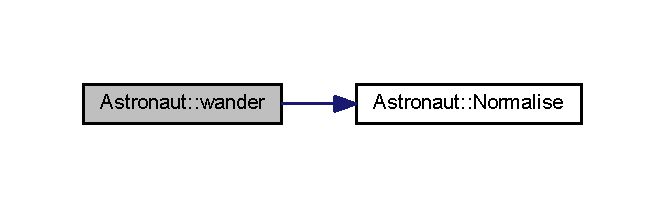
\includegraphics[width=319pt]{class_astronaut_a39d7e43f8604bf561570e2eb2564a8fa_cgraph}
\end{center}
\end{figure}
Here is the caller graph for this function\+:
\nopagebreak
\begin{figure}[H]
\begin{center}
\leavevmode
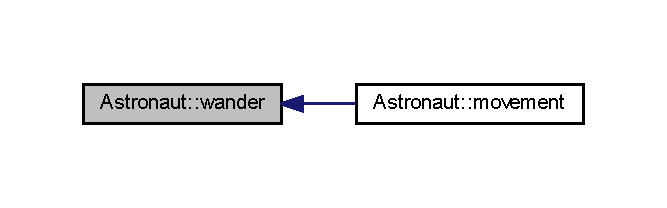
\includegraphics[width=320pt]{class_astronaut_a39d7e43f8604bf561570e2eb2564a8fa_icgraph}
\end{center}
\end{figure}


The documentation for this class was generated from the following files\+:\begin{DoxyCompactItemize}
\item 
\hyperlink{_astronaut_8h}{Astronaut.\+h}\item 
\hyperlink{_astronaut_8cpp}{Astronaut.\+cpp}\end{DoxyCompactItemize}

\hypertarget{class_bullet}{}\section{Bullet Class Reference}
\label{class_bullet}\index{Bullet@{Bullet}}


{\ttfamily \#include $<$Bullet.\+h$>$}



Collaboration diagram for Bullet\+:
\nopagebreak
\begin{figure}[H]
\begin{center}
\leavevmode
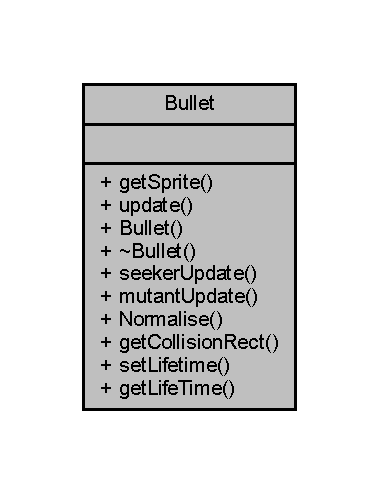
\includegraphics[width=182pt]{class_bullet__coll__graph}
\end{center}
\end{figure}
\subsection*{Public Member Functions}
\begin{DoxyCompactItemize}
\item 
sf\+::\+Sprite \hyperlink{class_bullet_aa313bc0e2c9fd200c526cb6fe320462c}{get\+Sprite} ()
\item 
void \hyperlink{class_bullet_a32f4a0611fe2dd245fee955d14ca1f68}{update} ()
\item 
\hyperlink{class_bullet_a479ca2fa9508190c8900f64584cbd7a0}{Bullet} (sf\+::\+Vector2f \+\_\+pos, sf\+::\+Vector2f \+\_\+vel, sf\+::\+Texture \+\_\+tex, float \+\_\+speed)
\item 
\hyperlink{class_bullet_aaeb5cb41d7db89f49007b08b41f1bfcf}{$\sim$\+Bullet} ()
\item 
void \hyperlink{class_bullet_add6e90fd23ded0a93ceaa2d489060591}{seeker\+Update} (sf\+::\+Vector2f target\+Pos)
\item 
void \hyperlink{class_bullet_a3af27cff51b293953e03bd4b749b6b8d}{mutant\+Update} (sf\+::\+Vector2f target\+Pos)
\item 
sf\+::\+Vector2f \hyperlink{class_bullet_a77e05d1fe031b205bfcfa388b13820c4}{Normalise} (sf\+::\+Vector2f velocity)
\item 
sf\+::\+Rectangle\+Shape \hyperlink{class_bullet_afa5ea4cb422dad6a578071ee86494a28}{get\+Collision\+Rect} ()
\item 
void \hyperlink{class_bullet_ae26b908cf0b00513a84cbfeb6582dfed}{set\+Lifetime} (int value)
\item 
int \hyperlink{class_bullet_a974be9eb4bd0cba53f578c7160fe2f87}{get\+Life\+Time} ()
\end{DoxyCompactItemize}


\subsection{Constructor \& Destructor Documentation}
\mbox{\Hypertarget{class_bullet_a479ca2fa9508190c8900f64584cbd7a0}\label{class_bullet_a479ca2fa9508190c8900f64584cbd7a0}} 
\index{Bullet@{Bullet}!Bullet@{Bullet}}
\index{Bullet@{Bullet}!Bullet@{Bullet}}
\subsubsection{\texorpdfstring{Bullet()}{Bullet()}}
{\footnotesize\ttfamily Bullet\+::\+Bullet (\begin{DoxyParamCaption}\item[{sf\+::\+Vector2f}]{\+\_\+pos,  }\item[{sf\+::\+Vector2f}]{\+\_\+vel,  }\item[{sf\+::\+Texture}]{\+\_\+tex,  }\item[{float}]{\+\_\+speed }\end{DoxyParamCaption})}

\mbox{\Hypertarget{class_bullet_aaeb5cb41d7db89f49007b08b41f1bfcf}\label{class_bullet_aaeb5cb41d7db89f49007b08b41f1bfcf}} 
\index{Bullet@{Bullet}!````~Bullet@{$\sim$\+Bullet}}
\index{````~Bullet@{$\sim$\+Bullet}!Bullet@{Bullet}}
\subsubsection{\texorpdfstring{$\sim$\+Bullet()}{~Bullet()}}
{\footnotesize\ttfamily Bullet\+::$\sim$\+Bullet (\begin{DoxyParamCaption}{ }\end{DoxyParamCaption})}



\subsection{Member Function Documentation}
\mbox{\Hypertarget{class_bullet_afa5ea4cb422dad6a578071ee86494a28}\label{class_bullet_afa5ea4cb422dad6a578071ee86494a28}} 
\index{Bullet@{Bullet}!get\+Collision\+Rect@{get\+Collision\+Rect}}
\index{get\+Collision\+Rect@{get\+Collision\+Rect}!Bullet@{Bullet}}
\subsubsection{\texorpdfstring{get\+Collision\+Rect()}{getCollisionRect()}}
{\footnotesize\ttfamily sf\+::\+Rectangle\+Shape Bullet\+::get\+Collision\+Rect (\begin{DoxyParamCaption}{ }\end{DoxyParamCaption})}

\mbox{\Hypertarget{class_bullet_a974be9eb4bd0cba53f578c7160fe2f87}\label{class_bullet_a974be9eb4bd0cba53f578c7160fe2f87}} 
\index{Bullet@{Bullet}!get\+Life\+Time@{get\+Life\+Time}}
\index{get\+Life\+Time@{get\+Life\+Time}!Bullet@{Bullet}}
\subsubsection{\texorpdfstring{get\+Life\+Time()}{getLifeTime()}}
{\footnotesize\ttfamily int Bullet\+::get\+Life\+Time (\begin{DoxyParamCaption}{ }\end{DoxyParamCaption})}

\mbox{\Hypertarget{class_bullet_aa313bc0e2c9fd200c526cb6fe320462c}\label{class_bullet_aa313bc0e2c9fd200c526cb6fe320462c}} 
\index{Bullet@{Bullet}!get\+Sprite@{get\+Sprite}}
\index{get\+Sprite@{get\+Sprite}!Bullet@{Bullet}}
\subsubsection{\texorpdfstring{get\+Sprite()}{getSprite()}}
{\footnotesize\ttfamily sf\+::\+Sprite Bullet\+::get\+Sprite (\begin{DoxyParamCaption}{ }\end{DoxyParamCaption})}

\mbox{\Hypertarget{class_bullet_a3af27cff51b293953e03bd4b749b6b8d}\label{class_bullet_a3af27cff51b293953e03bd4b749b6b8d}} 
\index{Bullet@{Bullet}!mutant\+Update@{mutant\+Update}}
\index{mutant\+Update@{mutant\+Update}!Bullet@{Bullet}}
\subsubsection{\texorpdfstring{mutant\+Update()}{mutantUpdate()}}
{\footnotesize\ttfamily void Bullet\+::mutant\+Update (\begin{DoxyParamCaption}\item[{sf\+::\+Vector2f}]{target\+Pos }\end{DoxyParamCaption})}

Here is the call graph for this function\+:
\nopagebreak
\begin{figure}[H]
\begin{center}
\leavevmode
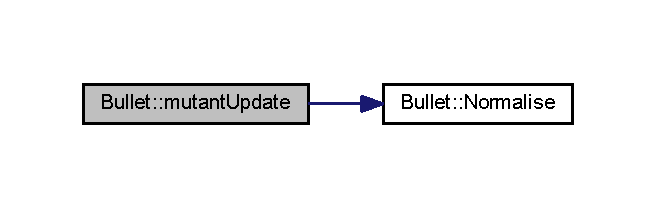
\includegraphics[width=315pt]{class_bullet_a3af27cff51b293953e03bd4b749b6b8d_cgraph}
\end{center}
\end{figure}
\mbox{\Hypertarget{class_bullet_a77e05d1fe031b205bfcfa388b13820c4}\label{class_bullet_a77e05d1fe031b205bfcfa388b13820c4}} 
\index{Bullet@{Bullet}!Normalise@{Normalise}}
\index{Normalise@{Normalise}!Bullet@{Bullet}}
\subsubsection{\texorpdfstring{Normalise()}{Normalise()}}
{\footnotesize\ttfamily sf\+::\+Vector2f Bullet\+::\+Normalise (\begin{DoxyParamCaption}\item[{sf\+::\+Vector2f}]{velocity }\end{DoxyParamCaption})}

Here is the caller graph for this function\+:
\nopagebreak
\begin{figure}[H]
\begin{center}
\leavevmode
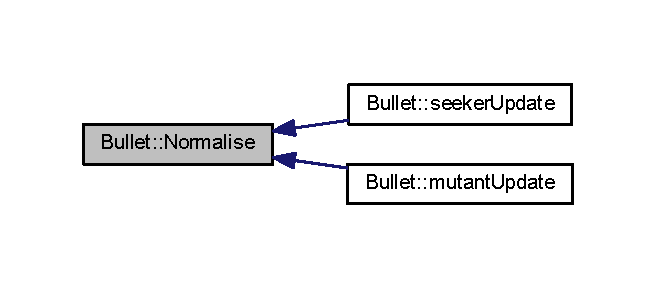
\includegraphics[width=315pt]{class_bullet_a77e05d1fe031b205bfcfa388b13820c4_icgraph}
\end{center}
\end{figure}
\mbox{\Hypertarget{class_bullet_add6e90fd23ded0a93ceaa2d489060591}\label{class_bullet_add6e90fd23ded0a93ceaa2d489060591}} 
\index{Bullet@{Bullet}!seeker\+Update@{seeker\+Update}}
\index{seeker\+Update@{seeker\+Update}!Bullet@{Bullet}}
\subsubsection{\texorpdfstring{seeker\+Update()}{seekerUpdate()}}
{\footnotesize\ttfamily void Bullet\+::seeker\+Update (\begin{DoxyParamCaption}\item[{sf\+::\+Vector2f}]{target\+Pos }\end{DoxyParamCaption})}

Here is the call graph for this function\+:
\nopagebreak
\begin{figure}[H]
\begin{center}
\leavevmode
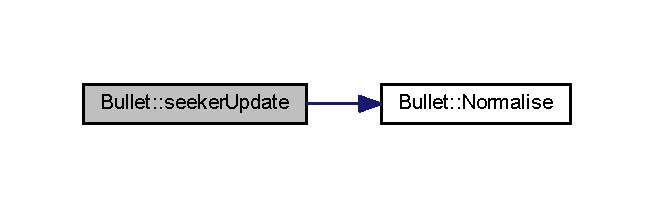
\includegraphics[width=314pt]{class_bullet_add6e90fd23ded0a93ceaa2d489060591_cgraph}
\end{center}
\end{figure}
\mbox{\Hypertarget{class_bullet_ae26b908cf0b00513a84cbfeb6582dfed}\label{class_bullet_ae26b908cf0b00513a84cbfeb6582dfed}} 
\index{Bullet@{Bullet}!set\+Lifetime@{set\+Lifetime}}
\index{set\+Lifetime@{set\+Lifetime}!Bullet@{Bullet}}
\subsubsection{\texorpdfstring{set\+Lifetime()}{setLifetime()}}
{\footnotesize\ttfamily void Bullet\+::set\+Lifetime (\begin{DoxyParamCaption}\item[{int}]{value }\end{DoxyParamCaption})}

\mbox{\Hypertarget{class_bullet_a32f4a0611fe2dd245fee955d14ca1f68}\label{class_bullet_a32f4a0611fe2dd245fee955d14ca1f68}} 
\index{Bullet@{Bullet}!update@{update}}
\index{update@{update}!Bullet@{Bullet}}
\subsubsection{\texorpdfstring{update()}{update()}}
{\footnotesize\ttfamily void Bullet\+::update (\begin{DoxyParamCaption}{ }\end{DoxyParamCaption})}



The documentation for this class was generated from the following files\+:\begin{DoxyCompactItemize}
\item 
\hyperlink{_bullet_8h}{Bullet.\+h}\item 
\hyperlink{_bullet_8cpp}{Bullet.\+cpp}\end{DoxyCompactItemize}

\hypertarget{class_collision_manager}{}\section{Collision\+Manager Class Reference}
\label{class_collision_manager}\index{Collision\+Manager@{Collision\+Manager}}


{\ttfamily \#include $<$Collision\+Manager.\+h$>$}



Collaboration diagram for Collision\+Manager\+:
\nopagebreak
\begin{figure}[H]
\begin{center}
\leavevmode
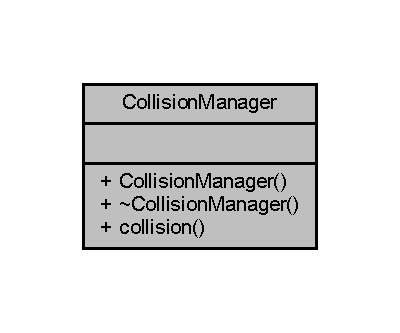
\includegraphics[width=192pt]{class_collision_manager__coll__graph}
\end{center}
\end{figure}
\subsection*{Public Member Functions}
\begin{DoxyCompactItemize}
\item 
\hyperlink{class_collision_manager_a81f0b3f0cc0268c80f54714cd7ddb55f}{Collision\+Manager} ()
\item 
\hyperlink{class_collision_manager_acdbb3c842f0ef1c7a028d3f080855766}{$\sim$\+Collision\+Manager} ()
\item 
bool \hyperlink{class_collision_manager_affe670241642e07380fff0050d8ef459}{collision} (sf\+::\+Rectangle\+Shape, sf\+::\+Rectangle\+Shape)
\end{DoxyCompactItemize}


\subsection{Constructor \& Destructor Documentation}
\mbox{\Hypertarget{class_collision_manager_a81f0b3f0cc0268c80f54714cd7ddb55f}\label{class_collision_manager_a81f0b3f0cc0268c80f54714cd7ddb55f}} 
\index{Collision\+Manager@{Collision\+Manager}!Collision\+Manager@{Collision\+Manager}}
\index{Collision\+Manager@{Collision\+Manager}!Collision\+Manager@{Collision\+Manager}}
\subsubsection{\texorpdfstring{Collision\+Manager()}{CollisionManager()}}
{\footnotesize\ttfamily Collision\+Manager\+::\+Collision\+Manager (\begin{DoxyParamCaption}{ }\end{DoxyParamCaption})}

\mbox{\Hypertarget{class_collision_manager_acdbb3c842f0ef1c7a028d3f080855766}\label{class_collision_manager_acdbb3c842f0ef1c7a028d3f080855766}} 
\index{Collision\+Manager@{Collision\+Manager}!````~Collision\+Manager@{$\sim$\+Collision\+Manager}}
\index{````~Collision\+Manager@{$\sim$\+Collision\+Manager}!Collision\+Manager@{Collision\+Manager}}
\subsubsection{\texorpdfstring{$\sim$\+Collision\+Manager()}{~CollisionManager()}}
{\footnotesize\ttfamily Collision\+Manager\+::$\sim$\+Collision\+Manager (\begin{DoxyParamCaption}{ }\end{DoxyParamCaption})}



\subsection{Member Function Documentation}
\mbox{\Hypertarget{class_collision_manager_affe670241642e07380fff0050d8ef459}\label{class_collision_manager_affe670241642e07380fff0050d8ef459}} 
\index{Collision\+Manager@{Collision\+Manager}!collision@{collision}}
\index{collision@{collision}!Collision\+Manager@{Collision\+Manager}}
\subsubsection{\texorpdfstring{collision()}{collision()}}
{\footnotesize\ttfamily bool Collision\+Manager\+::collision (\begin{DoxyParamCaption}\item[{sf\+::\+Rectangle\+Shape}]{\+\_\+rect1,  }\item[{sf\+::\+Rectangle\+Shape}]{\+\_\+rect2 }\end{DoxyParamCaption})}

Here is the caller graph for this function\+:
\nopagebreak
\begin{figure}[H]
\begin{center}
\leavevmode
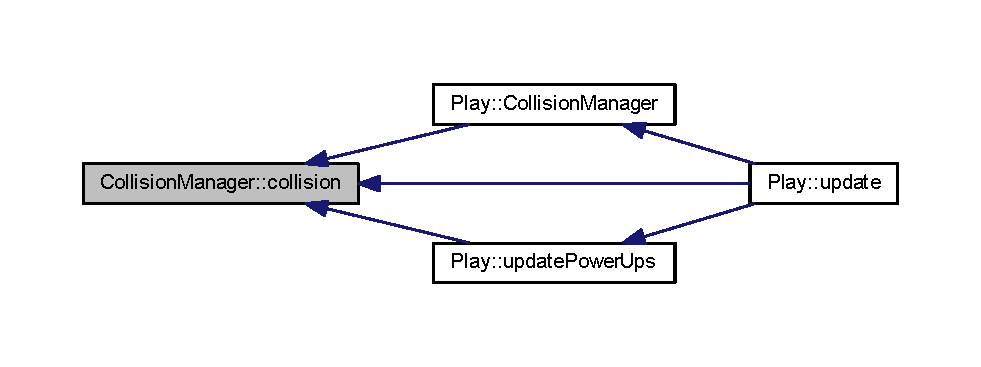
\includegraphics[width=350pt]{class_collision_manager_affe670241642e07380fff0050d8ef459_icgraph}
\end{center}
\end{figure}


The documentation for this class was generated from the following files\+:\begin{DoxyCompactItemize}
\item 
\hyperlink{_collision_manager_8h}{Collision\+Manager.\+h}\item 
\hyperlink{_collision_manager_8cpp}{Collision\+Manager.\+cpp}\end{DoxyCompactItemize}

\hypertarget{class_game}{}\section{Game Class Reference}
\label{class_game}\index{Game@{Game}}


{\ttfamily \#include $<$game.\+hpp$>$}



Collaboration diagram for Game\+:
\nopagebreak
\begin{figure}[H]
\begin{center}
\leavevmode
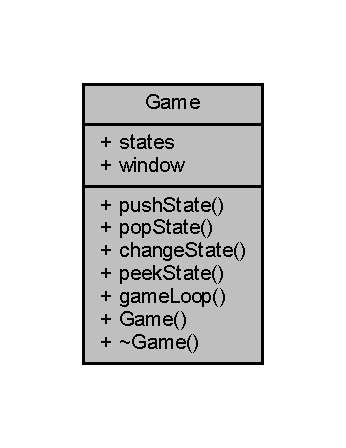
\includegraphics[width=166pt]{class_game__coll__graph}
\end{center}
\end{figure}
\subsection*{Public Member Functions}
\begin{DoxyCompactItemize}
\item 
void \hyperlink{class_game_a5898f1edb6e3bc1700b2ffb1943bc609}{push\+State} (\hyperlink{class_game_state}{Game\+State} $\ast$state)
\item 
void \hyperlink{class_game_a4b33dd67adef59bebadba8a234282c88}{pop\+State} ()
\item 
void \hyperlink{class_game_a8683b16995200bd11d95efc372e6722a}{change\+State} (\hyperlink{class_game_state}{Game\+State} $\ast$state)
\item 
\hyperlink{class_game_state}{Game\+State} $\ast$ \hyperlink{class_game_a6cdc6cb374ab8e7d8ac9b280284b3793}{peek\+State} ()
\item 
void \hyperlink{class_game_aede5f46c8c7bbbaf8459eeec397a11e7}{game\+Loop} ()
\item 
\hyperlink{class_game_ad59df6562a58a614fda24622d3715b65}{Game} ()
\item 
\hyperlink{class_game_ae3d112ca6e0e55150d2fdbc704474530}{$\sim$\+Game} ()
\end{DoxyCompactItemize}
\subsection*{Public Attributes}
\begin{DoxyCompactItemize}
\item 
std\+::stack$<$ \hyperlink{class_game_state}{Game\+State} $\ast$ $>$ \hyperlink{class_game_afb615f4fb6621cd14769c14716f4b0a5}{states}
\item 
sf\+::\+Render\+Window \hyperlink{class_game_a223de215aeb661cd423ac145756cc730}{window}
\end{DoxyCompactItemize}


\subsection{Constructor \& Destructor Documentation}
\mbox{\Hypertarget{class_game_ad59df6562a58a614fda24622d3715b65}\label{class_game_ad59df6562a58a614fda24622d3715b65}} 
\index{Game@{Game}!Game@{Game}}
\index{Game@{Game}!Game@{Game}}
\subsubsection{\texorpdfstring{Game()}{Game()}}
{\footnotesize\ttfamily Game\+::\+Game (\begin{DoxyParamCaption}{ }\end{DoxyParamCaption})}

\mbox{\Hypertarget{class_game_ae3d112ca6e0e55150d2fdbc704474530}\label{class_game_ae3d112ca6e0e55150d2fdbc704474530}} 
\index{Game@{Game}!````~Game@{$\sim$\+Game}}
\index{````~Game@{$\sim$\+Game}!Game@{Game}}
\subsubsection{\texorpdfstring{$\sim$\+Game()}{~Game()}}
{\footnotesize\ttfamily Game\+::$\sim$\+Game (\begin{DoxyParamCaption}{ }\end{DoxyParamCaption})}

Here is the call graph for this function\+:
\nopagebreak
\begin{figure}[H]
\begin{center}
\leavevmode
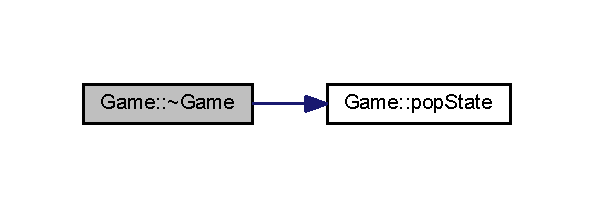
\includegraphics[width=285pt]{class_game_ae3d112ca6e0e55150d2fdbc704474530_cgraph}
\end{center}
\end{figure}


\subsection{Member Function Documentation}
\mbox{\Hypertarget{class_game_a8683b16995200bd11d95efc372e6722a}\label{class_game_a8683b16995200bd11d95efc372e6722a}} 
\index{Game@{Game}!change\+State@{change\+State}}
\index{change\+State@{change\+State}!Game@{Game}}
\subsubsection{\texorpdfstring{change\+State()}{changeState()}}
{\footnotesize\ttfamily void Game\+::change\+State (\begin{DoxyParamCaption}\item[{\hyperlink{class_game_state}{Game\+State} $\ast$}]{state }\end{DoxyParamCaption})}

Here is the call graph for this function\+:
\nopagebreak
\begin{figure}[H]
\begin{center}
\leavevmode
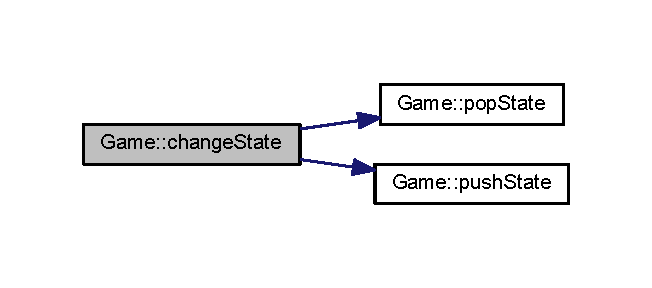
\includegraphics[width=313pt]{class_game_a8683b16995200bd11d95efc372e6722a_cgraph}
\end{center}
\end{figure}
Here is the caller graph for this function\+:
\nopagebreak
\begin{figure}[H]
\begin{center}
\leavevmode
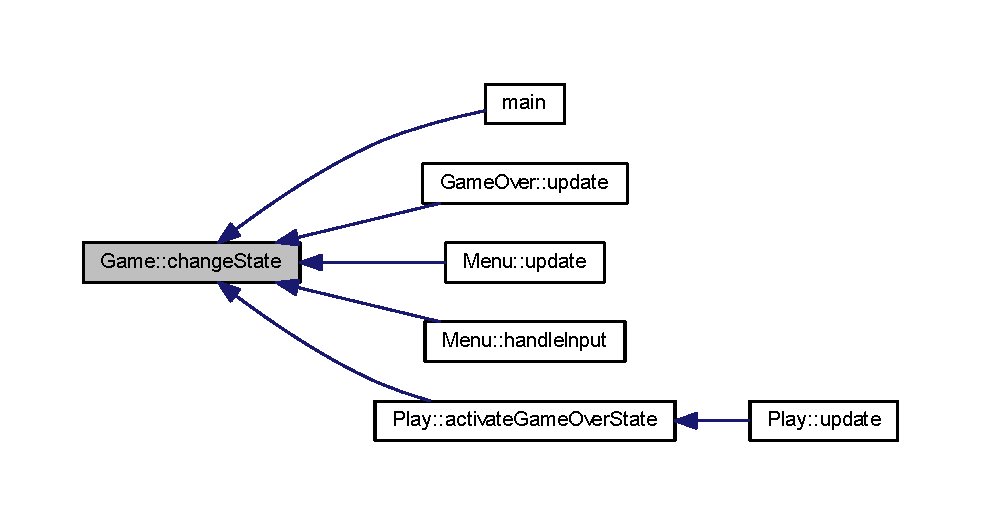
\includegraphics[width=350pt]{class_game_a8683b16995200bd11d95efc372e6722a_icgraph}
\end{center}
\end{figure}
\mbox{\Hypertarget{class_game_aede5f46c8c7bbbaf8459eeec397a11e7}\label{class_game_aede5f46c8c7bbbaf8459eeec397a11e7}} 
\index{Game@{Game}!game\+Loop@{game\+Loop}}
\index{game\+Loop@{game\+Loop}!Game@{Game}}
\subsubsection{\texorpdfstring{game\+Loop()}{gameLoop()}}
{\footnotesize\ttfamily void Game\+::game\+Loop (\begin{DoxyParamCaption}{ }\end{DoxyParamCaption})}

Here is the call graph for this function\+:
\nopagebreak
\begin{figure}[H]
\begin{center}
\leavevmode
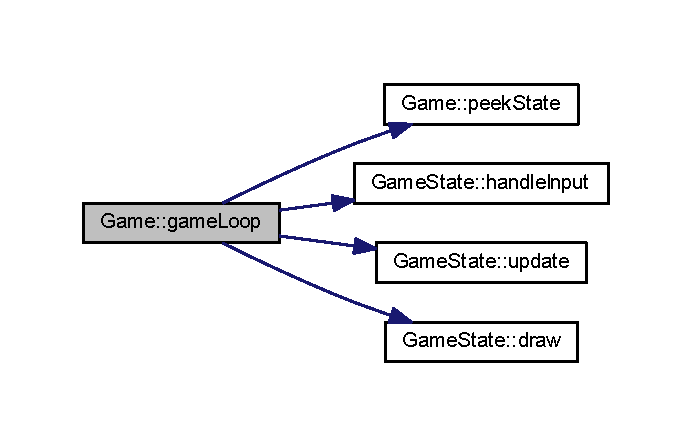
\includegraphics[width=332pt]{class_game_aede5f46c8c7bbbaf8459eeec397a11e7_cgraph}
\end{center}
\end{figure}
\mbox{\Hypertarget{class_game_a6cdc6cb374ab8e7d8ac9b280284b3793}\label{class_game_a6cdc6cb374ab8e7d8ac9b280284b3793}} 
\index{Game@{Game}!peek\+State@{peek\+State}}
\index{peek\+State@{peek\+State}!Game@{Game}}
\subsubsection{\texorpdfstring{peek\+State()}{peekState()}}
{\footnotesize\ttfamily \hyperlink{class_game_state}{Game\+State} $\ast$ Game\+::peek\+State (\begin{DoxyParamCaption}{ }\end{DoxyParamCaption})}

Here is the caller graph for this function\+:
\nopagebreak
\begin{figure}[H]
\begin{center}
\leavevmode
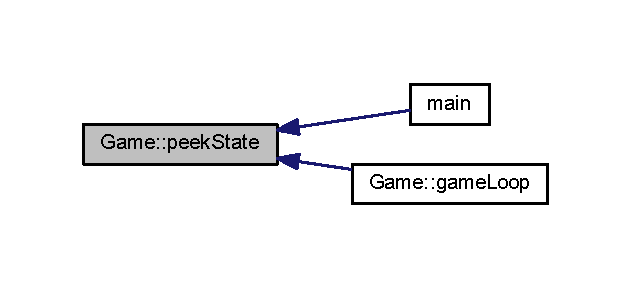
\includegraphics[width=303pt]{class_game_a6cdc6cb374ab8e7d8ac9b280284b3793_icgraph}
\end{center}
\end{figure}
\mbox{\Hypertarget{class_game_a4b33dd67adef59bebadba8a234282c88}\label{class_game_a4b33dd67adef59bebadba8a234282c88}} 
\index{Game@{Game}!pop\+State@{pop\+State}}
\index{pop\+State@{pop\+State}!Game@{Game}}
\subsubsection{\texorpdfstring{pop\+State()}{popState()}}
{\footnotesize\ttfamily void Game\+::pop\+State (\begin{DoxyParamCaption}{ }\end{DoxyParamCaption})}

Here is the caller graph for this function\+:
\nopagebreak
\begin{figure}[H]
\begin{center}
\leavevmode
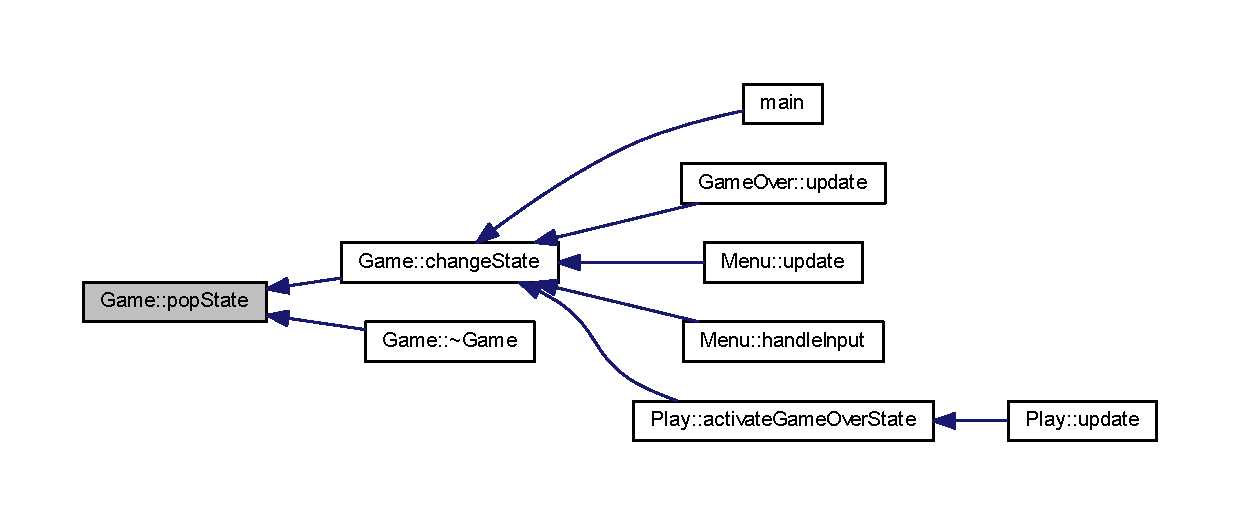
\includegraphics[width=350pt]{class_game_a4b33dd67adef59bebadba8a234282c88_icgraph}
\end{center}
\end{figure}
\mbox{\Hypertarget{class_game_a5898f1edb6e3bc1700b2ffb1943bc609}\label{class_game_a5898f1edb6e3bc1700b2ffb1943bc609}} 
\index{Game@{Game}!push\+State@{push\+State}}
\index{push\+State@{push\+State}!Game@{Game}}
\subsubsection{\texorpdfstring{push\+State()}{pushState()}}
{\footnotesize\ttfamily void Game\+::push\+State (\begin{DoxyParamCaption}\item[{\hyperlink{class_game_state}{Game\+State} $\ast$}]{state }\end{DoxyParamCaption})}

Here is the caller graph for this function\+:
\nopagebreak
\begin{figure}[H]
\begin{center}
\leavevmode
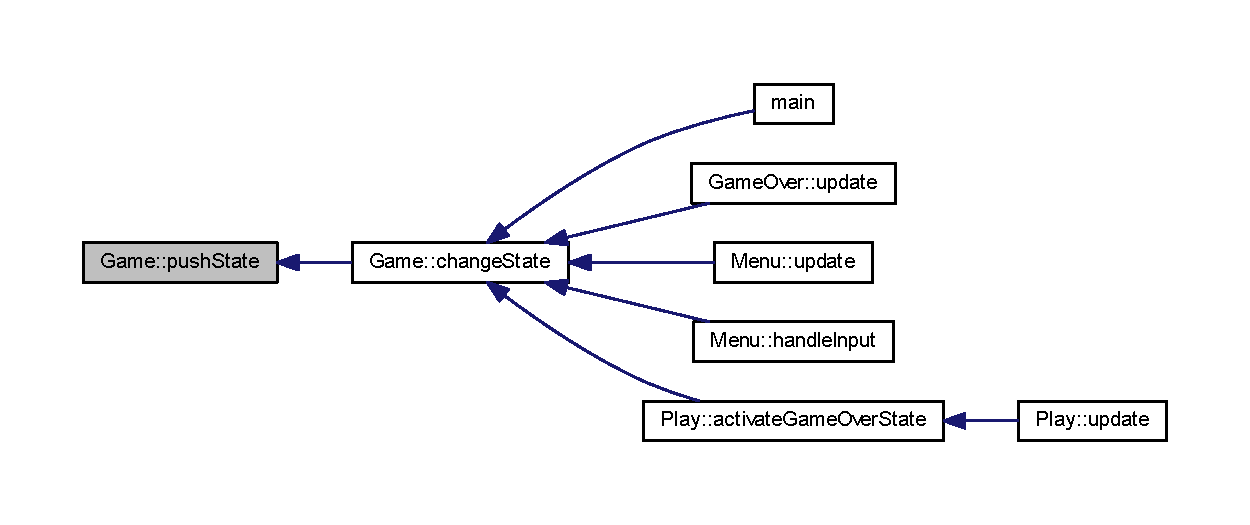
\includegraphics[width=350pt]{class_game_a5898f1edb6e3bc1700b2ffb1943bc609_icgraph}
\end{center}
\end{figure}


\subsection{Member Data Documentation}
\mbox{\Hypertarget{class_game_afb615f4fb6621cd14769c14716f4b0a5}\label{class_game_afb615f4fb6621cd14769c14716f4b0a5}} 
\index{Game@{Game}!states@{states}}
\index{states@{states}!Game@{Game}}
\subsubsection{\texorpdfstring{states}{states}}
{\footnotesize\ttfamily std\+::stack$<$\hyperlink{class_game_state}{Game\+State}$\ast$$>$ Game\+::states}

\mbox{\Hypertarget{class_game_a223de215aeb661cd423ac145756cc730}\label{class_game_a223de215aeb661cd423ac145756cc730}} 
\index{Game@{Game}!window@{window}}
\index{window@{window}!Game@{Game}}
\subsubsection{\texorpdfstring{window}{window}}
{\footnotesize\ttfamily sf\+::\+Render\+Window Game\+::window}



The documentation for this class was generated from the following files\+:\begin{DoxyCompactItemize}
\item 
\hyperlink{game_8hpp}{game.\+hpp}\item 
\hyperlink{game_8cpp}{game.\+cpp}\end{DoxyCompactItemize}

\hypertarget{class_game_over}{}\section{Game\+Over Class Reference}
\label{class_game_over}\index{Game\+Over@{Game\+Over}}


{\ttfamily \#include $<$Game\+Over.\+h$>$}



Inheritance diagram for Game\+Over\+:
\nopagebreak
\begin{figure}[H]
\begin{center}
\leavevmode
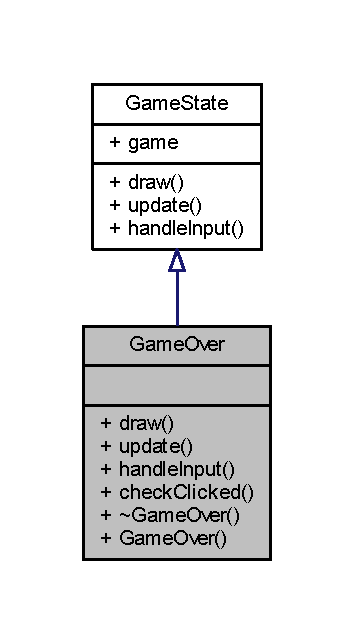
\includegraphics[width=170pt]{class_game_over__inherit__graph}
\end{center}
\end{figure}


Collaboration diagram for Game\+Over\+:
\nopagebreak
\begin{figure}[H]
\begin{center}
\leavevmode
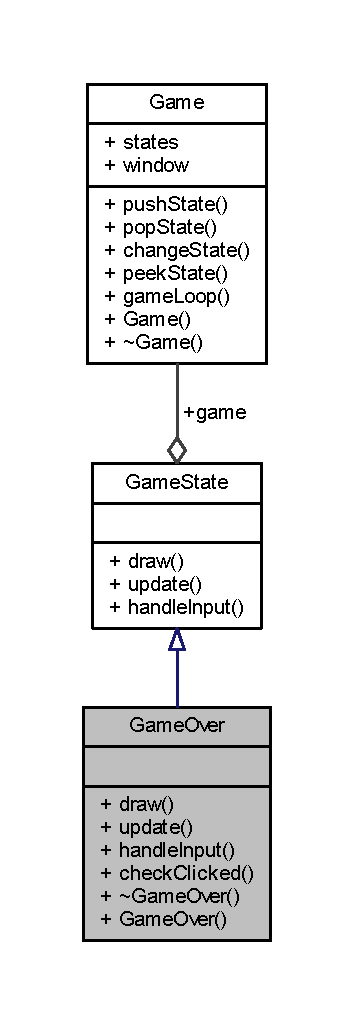
\includegraphics[width=170pt]{class_game_over__coll__graph}
\end{center}
\end{figure}
\subsection*{Public Member Functions}
\begin{DoxyCompactItemize}
\item 
virtual void \hyperlink{class_game_over_a250dc52de3aed814575b8f2df3ecbb06}{draw} ()
\item 
virtual void \hyperlink{class_game_over_a69f9e1364ff7caa8b17184441474c8b7}{update} ()
\item 
virtual void \hyperlink{class_game_over_acec786fec9ee289c9fab95b3b067efd0}{handle\+Input} ()
\item 
bool \hyperlink{class_game_over_a7239e22d93ea5a1374b5b75af3ed7ed6}{check\+Clicked} (sf\+::\+Sprite sprite, sf\+::\+Vector2i pos)
\item 
\hyperlink{class_game_over_ae36951a153d25d52fab7cbc7a85bbbbd}{$\sim$\+Game\+Over} ()
\item 
\hyperlink{class_game_over_aa3f05675e69ff44ac0f4edab4f3c2f14}{Game\+Over} (\hyperlink{class_game}{Game} $\ast$\hyperlink{class_game_state_a355a79415b9ef63c2aec1448a99f6e71}{game}, int)
\end{DoxyCompactItemize}
\subsection*{Additional Inherited Members}


\subsection{Constructor \& Destructor Documentation}
\mbox{\Hypertarget{class_game_over_ae36951a153d25d52fab7cbc7a85bbbbd}\label{class_game_over_ae36951a153d25d52fab7cbc7a85bbbbd}} 
\index{Game\+Over@{Game\+Over}!````~Game\+Over@{$\sim$\+Game\+Over}}
\index{````~Game\+Over@{$\sim$\+Game\+Over}!Game\+Over@{Game\+Over}}
\subsubsection{\texorpdfstring{$\sim$\+Game\+Over()}{~GameOver()}}
{\footnotesize\ttfamily Game\+Over\+::$\sim$\+Game\+Over (\begin{DoxyParamCaption}{ }\end{DoxyParamCaption})}

\mbox{\Hypertarget{class_game_over_aa3f05675e69ff44ac0f4edab4f3c2f14}\label{class_game_over_aa3f05675e69ff44ac0f4edab4f3c2f14}} 
\index{Game\+Over@{Game\+Over}!Game\+Over@{Game\+Over}}
\index{Game\+Over@{Game\+Over}!Game\+Over@{Game\+Over}}
\subsubsection{\texorpdfstring{Game\+Over()}{GameOver()}}
{\footnotesize\ttfamily Game\+Over\+::\+Game\+Over (\begin{DoxyParamCaption}\item[{\hyperlink{class_game}{Game} $\ast$}]{game,  }\item[{int}]{\+\_\+score }\end{DoxyParamCaption})}



\subsection{Member Function Documentation}
\mbox{\Hypertarget{class_game_over_a7239e22d93ea5a1374b5b75af3ed7ed6}\label{class_game_over_a7239e22d93ea5a1374b5b75af3ed7ed6}} 
\index{Game\+Over@{Game\+Over}!check\+Clicked@{check\+Clicked}}
\index{check\+Clicked@{check\+Clicked}!Game\+Over@{Game\+Over}}
\subsubsection{\texorpdfstring{check\+Clicked()}{checkClicked()}}
{\footnotesize\ttfamily bool Game\+Over\+::check\+Clicked (\begin{DoxyParamCaption}\item[{sf\+::\+Sprite}]{sprite,  }\item[{sf\+::\+Vector2i}]{pos }\end{DoxyParamCaption})}

Here is the caller graph for this function\+:
\nopagebreak
\begin{figure}[H]
\begin{center}
\leavevmode
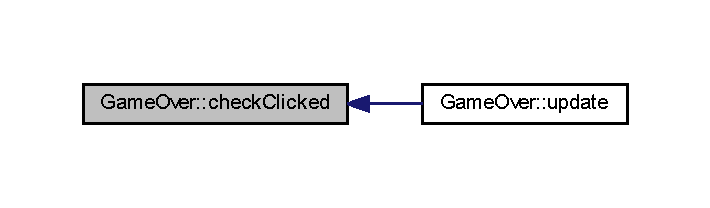
\includegraphics[width=341pt]{class_game_over_a7239e22d93ea5a1374b5b75af3ed7ed6_icgraph}
\end{center}
\end{figure}
\mbox{\Hypertarget{class_game_over_a250dc52de3aed814575b8f2df3ecbb06}\label{class_game_over_a250dc52de3aed814575b8f2df3ecbb06}} 
\index{Game\+Over@{Game\+Over}!draw@{draw}}
\index{draw@{draw}!Game\+Over@{Game\+Over}}
\subsubsection{\texorpdfstring{draw()}{draw()}}
{\footnotesize\ttfamily void Game\+Over\+::draw (\begin{DoxyParamCaption}{ }\end{DoxyParamCaption})\hspace{0.3cm}{\ttfamily [virtual]}}



Implements \hyperlink{class_game_state_ac872d748df12ac36d7a42a191997e4f7}{Game\+State}.

\mbox{\Hypertarget{class_game_over_acec786fec9ee289c9fab95b3b067efd0}\label{class_game_over_acec786fec9ee289c9fab95b3b067efd0}} 
\index{Game\+Over@{Game\+Over}!handle\+Input@{handle\+Input}}
\index{handle\+Input@{handle\+Input}!Game\+Over@{Game\+Over}}
\subsubsection{\texorpdfstring{handle\+Input()}{handleInput()}}
{\footnotesize\ttfamily void Game\+Over\+::handle\+Input (\begin{DoxyParamCaption}{ }\end{DoxyParamCaption})\hspace{0.3cm}{\ttfamily [virtual]}}



Implements \hyperlink{class_game_state_a970b55edd5a1da31ea0f7113e2c1f85a}{Game\+State}.

\mbox{\Hypertarget{class_game_over_a69f9e1364ff7caa8b17184441474c8b7}\label{class_game_over_a69f9e1364ff7caa8b17184441474c8b7}} 
\index{Game\+Over@{Game\+Over}!update@{update}}
\index{update@{update}!Game\+Over@{Game\+Over}}
\subsubsection{\texorpdfstring{update()}{update()}}
{\footnotesize\ttfamily void Game\+Over\+::update (\begin{DoxyParamCaption}{ }\end{DoxyParamCaption})\hspace{0.3cm}{\ttfamily [virtual]}}



Implements \hyperlink{class_game_state_ab2864bfa04f92f6966861a1f2883bda0}{Game\+State}.

Here is the call graph for this function\+:
\nopagebreak
\begin{figure}[H]
\begin{center}
\leavevmode
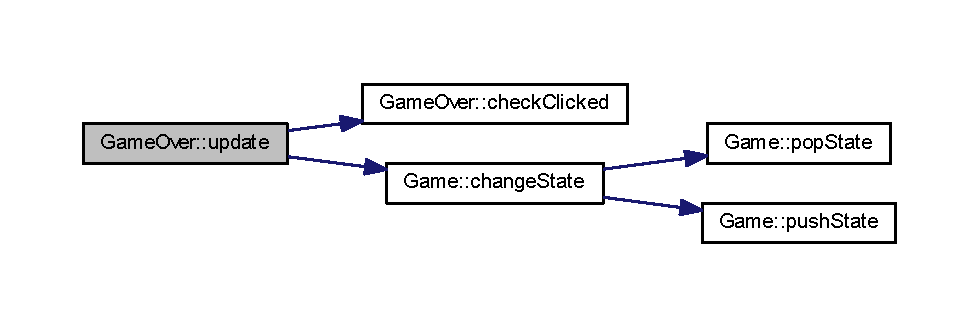
\includegraphics[width=350pt]{class_game_over_a69f9e1364ff7caa8b17184441474c8b7_cgraph}
\end{center}
\end{figure}


The documentation for this class was generated from the following files\+:\begin{DoxyCompactItemize}
\item 
\hyperlink{_game_over_8h}{Game\+Over.\+h}\item 
\hyperlink{_game_over_8cpp}{Game\+Over.\+cpp}\end{DoxyCompactItemize}

\hypertarget{class_game_state}{}\section{Game\+State Class Reference}
\label{class_game_state}\index{Game\+State@{Game\+State}}


{\ttfamily \#include $<$game\+\_\+state.\+hpp$>$}



Inheritance diagram for Game\+State\+:
\nopagebreak
\begin{figure}[H]
\begin{center}
\leavevmode
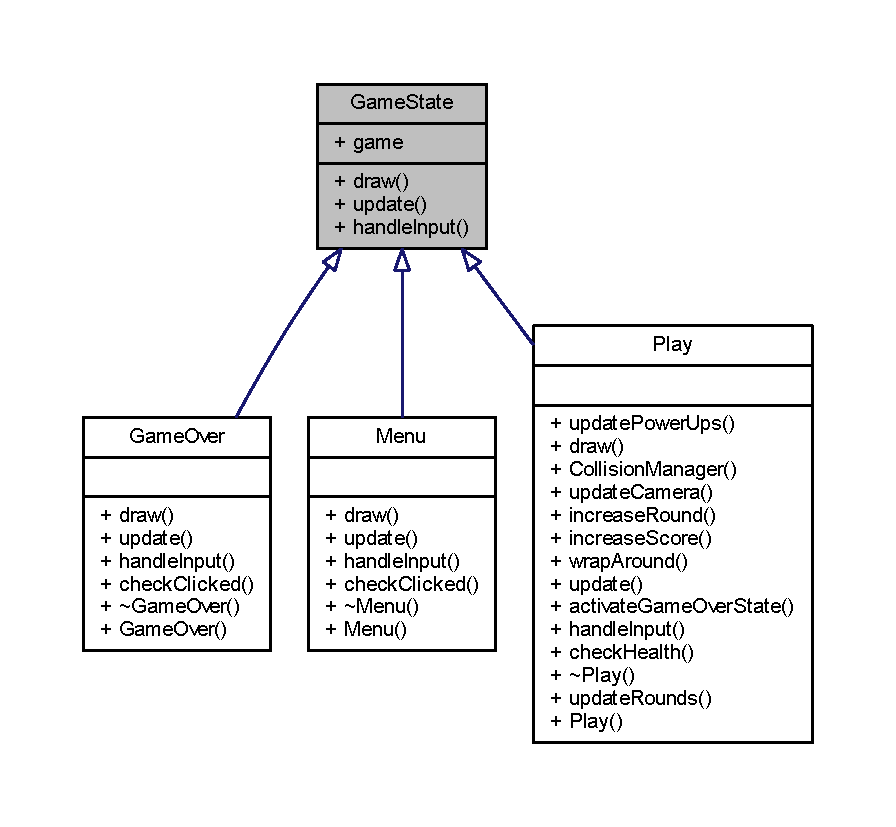
\includegraphics[width=350pt]{class_game_state__inherit__graph}
\end{center}
\end{figure}


Collaboration diagram for Game\+State\+:
\nopagebreak
\begin{figure}[H]
\begin{center}
\leavevmode
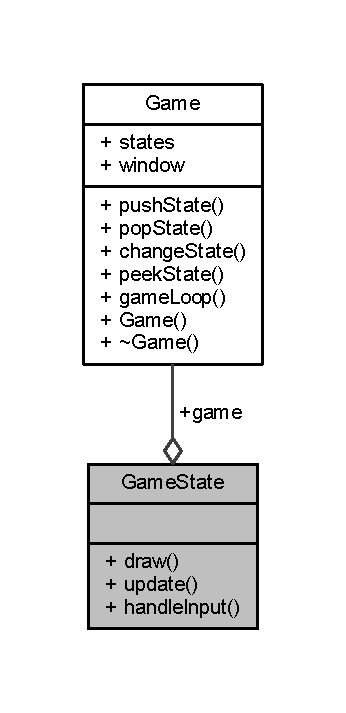
\includegraphics[width=166pt]{class_game_state__coll__graph}
\end{center}
\end{figure}
\subsection*{Public Member Functions}
\begin{DoxyCompactItemize}
\item 
virtual void \hyperlink{class_game_state_ac872d748df12ac36d7a42a191997e4f7}{draw} ()=0
\item 
virtual void \hyperlink{class_game_state_ab2864bfa04f92f6966861a1f2883bda0}{update} ()=0
\item 
virtual void \hyperlink{class_game_state_a970b55edd5a1da31ea0f7113e2c1f85a}{handle\+Input} ()=0
\end{DoxyCompactItemize}
\subsection*{Public Attributes}
\begin{DoxyCompactItemize}
\item 
\hyperlink{class_game}{Game} $\ast$ \hyperlink{class_game_state_a355a79415b9ef63c2aec1448a99f6e71}{game}
\end{DoxyCompactItemize}


\subsection{Member Function Documentation}
\mbox{\Hypertarget{class_game_state_ac872d748df12ac36d7a42a191997e4f7}\label{class_game_state_ac872d748df12ac36d7a42a191997e4f7}} 
\index{Game\+State@{Game\+State}!draw@{draw}}
\index{draw@{draw}!Game\+State@{Game\+State}}
\subsubsection{\texorpdfstring{draw()}{draw()}}
{\footnotesize\ttfamily virtual void Game\+State\+::draw (\begin{DoxyParamCaption}{ }\end{DoxyParamCaption})\hspace{0.3cm}{\ttfamily [pure virtual]}}



Implemented in \hyperlink{class_play_a026d1354c1b7ac0df50b7108c78aec61}{Play}, \hyperlink{class_game_over_a250dc52de3aed814575b8f2df3ecbb06}{Game\+Over}, and \hyperlink{class_menu_a2cd7ab9901a8f42a3ae977d0774398a6}{Menu}.

Here is the caller graph for this function\+:
\nopagebreak
\begin{figure}[H]
\begin{center}
\leavevmode
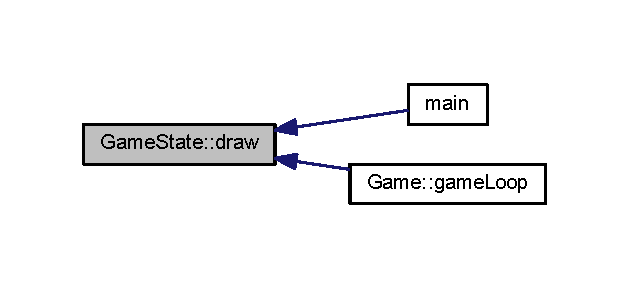
\includegraphics[width=302pt]{class_game_state_ac872d748df12ac36d7a42a191997e4f7_icgraph}
\end{center}
\end{figure}
\mbox{\Hypertarget{class_game_state_a970b55edd5a1da31ea0f7113e2c1f85a}\label{class_game_state_a970b55edd5a1da31ea0f7113e2c1f85a}} 
\index{Game\+State@{Game\+State}!handle\+Input@{handle\+Input}}
\index{handle\+Input@{handle\+Input}!Game\+State@{Game\+State}}
\subsubsection{\texorpdfstring{handle\+Input()}{handleInput()}}
{\footnotesize\ttfamily virtual void Game\+State\+::handle\+Input (\begin{DoxyParamCaption}{ }\end{DoxyParamCaption})\hspace{0.3cm}{\ttfamily [pure virtual]}}



Implemented in \hyperlink{class_play_a81bdbd1ef7b3de50dba1a8ebf346a1fc}{Play}, \hyperlink{class_game_over_acec786fec9ee289c9fab95b3b067efd0}{Game\+Over}, and \hyperlink{class_menu_a28296c3978c880ea9288fc97a869795d}{Menu}.

Here is the caller graph for this function\+:
\nopagebreak
\begin{figure}[H]
\begin{center}
\leavevmode
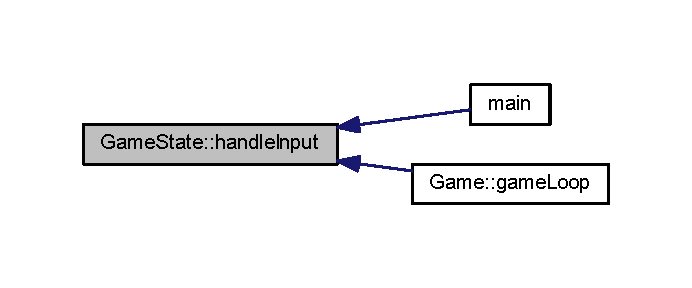
\includegraphics[width=332pt]{class_game_state_a970b55edd5a1da31ea0f7113e2c1f85a_icgraph}
\end{center}
\end{figure}
\mbox{\Hypertarget{class_game_state_ab2864bfa04f92f6966861a1f2883bda0}\label{class_game_state_ab2864bfa04f92f6966861a1f2883bda0}} 
\index{Game\+State@{Game\+State}!update@{update}}
\index{update@{update}!Game\+State@{Game\+State}}
\subsubsection{\texorpdfstring{update()}{update()}}
{\footnotesize\ttfamily virtual void Game\+State\+::update (\begin{DoxyParamCaption}{ }\end{DoxyParamCaption})\hspace{0.3cm}{\ttfamily [pure virtual]}}



Implemented in \hyperlink{class_play_a8eaa457d009e35bfbf699b38b569e3b8}{Play}, \hyperlink{class_game_over_a69f9e1364ff7caa8b17184441474c8b7}{Game\+Over}, and \hyperlink{class_menu_a8446e8a1e56e9cf1db93790067510a61}{Menu}.

Here is the caller graph for this function\+:
\nopagebreak
\begin{figure}[H]
\begin{center}
\leavevmode
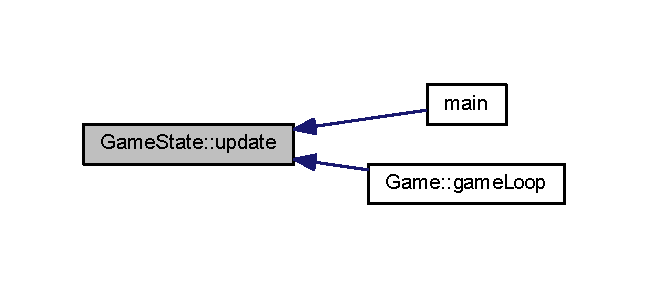
\includegraphics[width=311pt]{class_game_state_ab2864bfa04f92f6966861a1f2883bda0_icgraph}
\end{center}
\end{figure}


\subsection{Member Data Documentation}
\mbox{\Hypertarget{class_game_state_a355a79415b9ef63c2aec1448a99f6e71}\label{class_game_state_a355a79415b9ef63c2aec1448a99f6e71}} 
\index{Game\+State@{Game\+State}!game@{game}}
\index{game@{game}!Game\+State@{Game\+State}}
\subsubsection{\texorpdfstring{game}{game}}
{\footnotesize\ttfamily \hyperlink{class_game}{Game}$\ast$ Game\+State\+::game}



The documentation for this class was generated from the following file\+:\begin{DoxyCompactItemize}
\item 
\hyperlink{game__state_8hpp}{game\+\_\+state.\+hpp}\end{DoxyCompactItemize}

\hypertarget{class_menu}{}\section{Menu Class Reference}
\label{class_menu}\index{Menu@{Menu}}


{\ttfamily \#include $<$Menu.\+hpp$>$}



Inheritance diagram for Menu\+:
\nopagebreak
\begin{figure}[H]
\begin{center}
\leavevmode
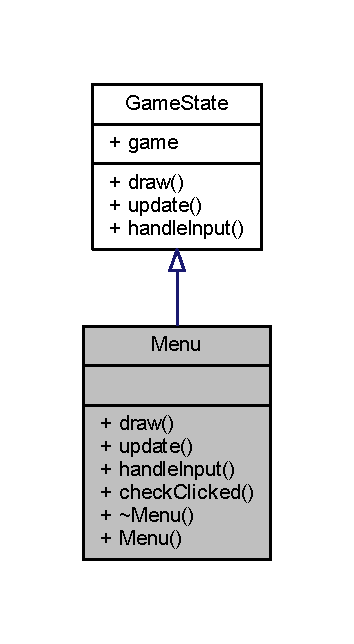
\includegraphics[width=170pt]{class_menu__inherit__graph}
\end{center}
\end{figure}


Collaboration diagram for Menu\+:
\nopagebreak
\begin{figure}[H]
\begin{center}
\leavevmode
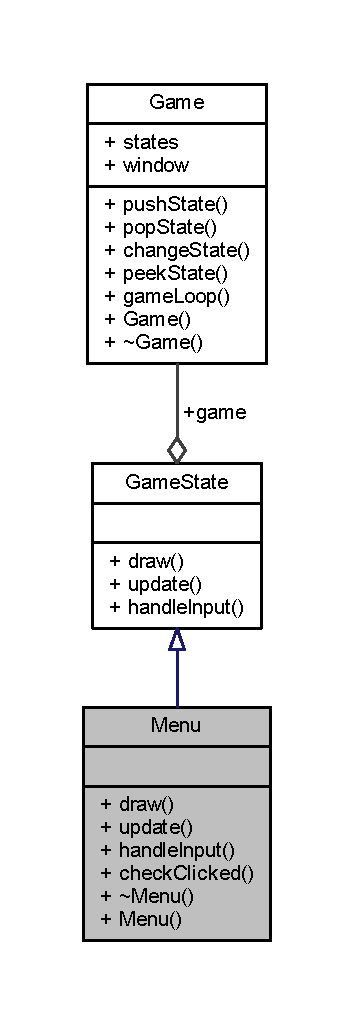
\includegraphics[width=170pt]{class_menu__coll__graph}
\end{center}
\end{figure}
\subsection*{Public Member Functions}
\begin{DoxyCompactItemize}
\item 
virtual void \hyperlink{class_menu_a2cd7ab9901a8f42a3ae977d0774398a6}{draw} ()
\item 
virtual void \hyperlink{class_menu_a8446e8a1e56e9cf1db93790067510a61}{update} ()
\item 
virtual void \hyperlink{class_menu_a28296c3978c880ea9288fc97a869795d}{handle\+Input} ()
\item 
bool \hyperlink{class_menu_a1b4d7af621c036afa3d9758e8accbc16}{check\+Clicked} (sf\+::\+Sprite sprite, sf\+::\+Vector2i pos)
\item 
\hyperlink{class_menu_a831387f51358cfb88cd018e1777bc980}{$\sim$\+Menu} ()
\item 
\hyperlink{class_menu_a91ec4975ad2aced80cd524a179dd7af1}{Menu} (\hyperlink{class_game}{Game} $\ast$\hyperlink{class_game_state_a355a79415b9ef63c2aec1448a99f6e71}{game})
\end{DoxyCompactItemize}
\subsection*{Additional Inherited Members}


\subsection{Constructor \& Destructor Documentation}
\mbox{\Hypertarget{class_menu_a831387f51358cfb88cd018e1777bc980}\label{class_menu_a831387f51358cfb88cd018e1777bc980}} 
\index{Menu@{Menu}!````~Menu@{$\sim$\+Menu}}
\index{````~Menu@{$\sim$\+Menu}!Menu@{Menu}}
\subsubsection{\texorpdfstring{$\sim$\+Menu()}{~Menu()}}
{\footnotesize\ttfamily Menu\+::$\sim$\+Menu (\begin{DoxyParamCaption}{ }\end{DoxyParamCaption})}

\mbox{\Hypertarget{class_menu_a91ec4975ad2aced80cd524a179dd7af1}\label{class_menu_a91ec4975ad2aced80cd524a179dd7af1}} 
\index{Menu@{Menu}!Menu@{Menu}}
\index{Menu@{Menu}!Menu@{Menu}}
\subsubsection{\texorpdfstring{Menu()}{Menu()}}
{\footnotesize\ttfamily Menu\+::\+Menu (\begin{DoxyParamCaption}\item[{\hyperlink{class_game}{Game} $\ast$}]{game }\end{DoxyParamCaption})}



\subsection{Member Function Documentation}
\mbox{\Hypertarget{class_menu_a1b4d7af621c036afa3d9758e8accbc16}\label{class_menu_a1b4d7af621c036afa3d9758e8accbc16}} 
\index{Menu@{Menu}!check\+Clicked@{check\+Clicked}}
\index{check\+Clicked@{check\+Clicked}!Menu@{Menu}}
\subsubsection{\texorpdfstring{check\+Clicked()}{checkClicked()}}
{\footnotesize\ttfamily bool Menu\+::check\+Clicked (\begin{DoxyParamCaption}\item[{sf\+::\+Sprite}]{sprite,  }\item[{sf\+::\+Vector2i}]{pos }\end{DoxyParamCaption})}

Here is the caller graph for this function\+:
\nopagebreak
\begin{figure}[H]
\begin{center}
\leavevmode
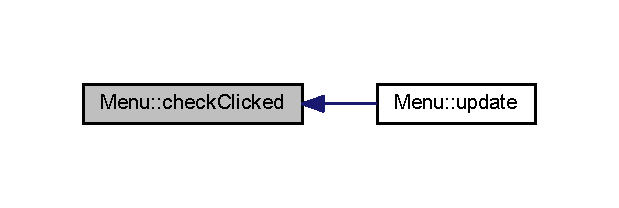
\includegraphics[width=297pt]{class_menu_a1b4d7af621c036afa3d9758e8accbc16_icgraph}
\end{center}
\end{figure}
\mbox{\Hypertarget{class_menu_a2cd7ab9901a8f42a3ae977d0774398a6}\label{class_menu_a2cd7ab9901a8f42a3ae977d0774398a6}} 
\index{Menu@{Menu}!draw@{draw}}
\index{draw@{draw}!Menu@{Menu}}
\subsubsection{\texorpdfstring{draw()}{draw()}}
{\footnotesize\ttfamily void Menu\+::draw (\begin{DoxyParamCaption}{ }\end{DoxyParamCaption})\hspace{0.3cm}{\ttfamily [virtual]}}



Implements \hyperlink{class_game_state_ac872d748df12ac36d7a42a191997e4f7}{Game\+State}.

\mbox{\Hypertarget{class_menu_a28296c3978c880ea9288fc97a869795d}\label{class_menu_a28296c3978c880ea9288fc97a869795d}} 
\index{Menu@{Menu}!handle\+Input@{handle\+Input}}
\index{handle\+Input@{handle\+Input}!Menu@{Menu}}
\subsubsection{\texorpdfstring{handle\+Input()}{handleInput()}}
{\footnotesize\ttfamily void Menu\+::handle\+Input (\begin{DoxyParamCaption}{ }\end{DoxyParamCaption})\hspace{0.3cm}{\ttfamily [virtual]}}



Implements \hyperlink{class_game_state_a970b55edd5a1da31ea0f7113e2c1f85a}{Game\+State}.

Here is the call graph for this function\+:
\nopagebreak
\begin{figure}[H]
\begin{center}
\leavevmode
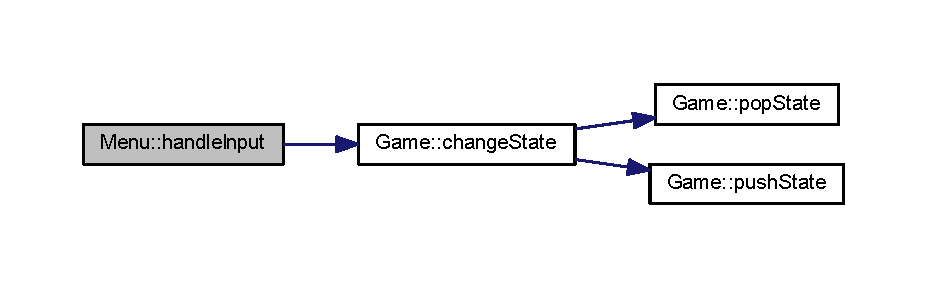
\includegraphics[width=350pt]{class_menu_a28296c3978c880ea9288fc97a869795d_cgraph}
\end{center}
\end{figure}
\mbox{\Hypertarget{class_menu_a8446e8a1e56e9cf1db93790067510a61}\label{class_menu_a8446e8a1e56e9cf1db93790067510a61}} 
\index{Menu@{Menu}!update@{update}}
\index{update@{update}!Menu@{Menu}}
\subsubsection{\texorpdfstring{update()}{update()}}
{\footnotesize\ttfamily void Menu\+::update (\begin{DoxyParamCaption}{ }\end{DoxyParamCaption})\hspace{0.3cm}{\ttfamily [virtual]}}



Implements \hyperlink{class_game_state_ab2864bfa04f92f6966861a1f2883bda0}{Game\+State}.

Here is the call graph for this function\+:
\nopagebreak
\begin{figure}[H]
\begin{center}
\leavevmode
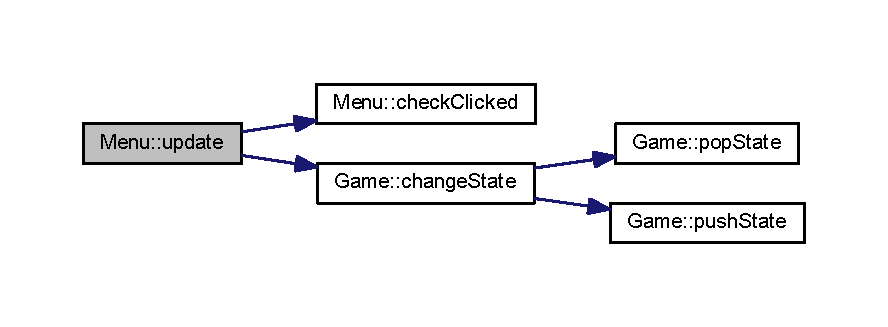
\includegraphics[width=350pt]{class_menu_a8446e8a1e56e9cf1db93790067510a61_cgraph}
\end{center}
\end{figure}


The documentation for this class was generated from the following files\+:\begin{DoxyCompactItemize}
\item 
\hyperlink{_menu_8hpp}{Menu.\+hpp}\item 
\hyperlink{_menu_8cpp}{Menu.\+cpp}\end{DoxyCompactItemize}

\hypertarget{class_mutant}{}\section{Mutant Class Reference}
\label{class_mutant}\index{Mutant@{Mutant}}


{\ttfamily \#include $<$Mutant.\+h$>$}



Collaboration diagram for Mutant\+:
\nopagebreak
\begin{figure}[H]
\begin{center}
\leavevmode
\includegraphics[width=196pt]{class_mutant__coll__graph}
\end{center}
\end{figure}
\subsection*{Public Member Functions}
\begin{DoxyCompactItemize}
\item 
\hyperlink{class_mutant_acbc96ca2187e5266adf4fdaca228eeb0}{Mutant} (sf\+::\+Vector2f \+\_\+pos, sf\+::\+Vector2f \+\_\+vel, sf\+::\+Texture \+\_\+tex)
\item 
\hyperlink{class_mutant_a03dc2cf4d08ea08bea6cd4ded784dfc1}{$\sim$\+Mutant} ()
\item 
sf\+::\+Vector2f \hyperlink{class_mutant_a7455d81b54b869ac1f466bfc08c44ebb}{get\+Velocity} ()
\item 
void \hyperlink{class_mutant_a66e452c4f98ebaed704b29127403d3d9}{setindex} (int value)
\item 
sf\+::\+Vector2f \hyperlink{class_mutant_a1c6dbda519e0d1fa4013478f0337ed96}{compute\+Alignment} (std\+::vector$<$ \hyperlink{class_mutant}{Mutant} $\ast$$>$ agents)
\item 
sf\+::\+Vector2f \hyperlink{class_mutant_ab6daf2a25a5a96ccc672ef00d3aa90d4}{compute\+Cohesion} (std\+::vector$<$ \hyperlink{class_mutant}{Mutant} $\ast$$>$ agents)
\item 
sf\+::\+Vector2f \hyperlink{class_mutant_a3477994ce821511033006866f2f3b987}{compute\+Separation} (std\+::vector$<$ \hyperlink{class_mutant}{Mutant} $\ast$$>$ agents)
\item 
sf\+::\+Vector2f \hyperlink{class_mutant_ab20f22800bae3c7587beb641248412ac}{get\+Position} ()
\item 
void \hyperlink{class_mutant_af815ec529e98bf10daa9ac346c87f4d0}{set\+Position} (sf\+::\+Vector2f \+\_\+temp\+Pos)
\item 
sf\+::\+Sprite \hyperlink{class_mutant_a16d41479b4fabb6efef0a1af6a2df6ff}{get\+Sprite} ()
\item 
sf\+::\+Rectangle\+Shape \hyperlink{class_mutant_ada703f83af37442914832a08333dab26}{get\+Collision\+Rect} ()
\item 
void \hyperlink{class_mutant_af76cac0ad55dd2d515736f76cf693f40}{update} ()
\item 
void \hyperlink{class_mutant_a24699eb054b6cf95f66bf3e856364b71}{seek} (sf\+::\+Vector2f target\+Pos)
\item 
sf\+::\+Vector2f \hyperlink{class_mutant_a167cab6fa9c2a19f40c9886f043c1270}{Normalise} (sf\+::\+Vector2f velocity)
\item 
void \hyperlink{class_mutant_a95c362ea2f31919f63047b872cfdaf20}{movement} (sf\+::\+Vector2f target\+Pos, sf\+::\+Texture \+\_\+player\+Bullet)
\item 
void \hyperlink{class_mutant_aaa71f2f6d0fe2be008db453bb9673d4c}{fire} (sf\+::\+Vector2f target\+Pos, sf\+::\+Texture \+\_\+player\+Bullet)
\item 
void \hyperlink{class_mutant_ab5f88d52695dfbece143049c81e9542d}{swarm} (std\+::vector$<$ \hyperlink{class_mutant}{Mutant} $\ast$$>$ agents, sf\+::\+Vector2f \+\_\+player\+Pos)
\item 
int \hyperlink{class_mutant_ae80452778ea58cf79ff76a1a481712af}{get\+Health} ()
\item 
void \hyperlink{class_mutant_ab03caeb2812412cee78692a29380a47b}{take\+Damage} (int value)
\item 
std\+::vector$<$ \hyperlink{class_bullet}{Bullet} $\ast$ $>$ \& \hyperlink{class_mutant_a0f42cf94b9b6fb45b292ce1fb4e3233f}{get\+Bullets} ()
\end{DoxyCompactItemize}


\subsection{Constructor \& Destructor Documentation}
\mbox{\Hypertarget{class_mutant_acbc96ca2187e5266adf4fdaca228eeb0}\label{class_mutant_acbc96ca2187e5266adf4fdaca228eeb0}} 
\index{Mutant@{Mutant}!Mutant@{Mutant}}
\index{Mutant@{Mutant}!Mutant@{Mutant}}
\subsubsection{\texorpdfstring{Mutant()}{Mutant()}}
{\footnotesize\ttfamily Mutant\+::\+Mutant (\begin{DoxyParamCaption}\item[{sf\+::\+Vector2f}]{\+\_\+pos,  }\item[{sf\+::\+Vector2f}]{\+\_\+vel,  }\item[{sf\+::\+Texture}]{\+\_\+tex }\end{DoxyParamCaption})}

\mbox{\Hypertarget{class_mutant_a03dc2cf4d08ea08bea6cd4ded784dfc1}\label{class_mutant_a03dc2cf4d08ea08bea6cd4ded784dfc1}} 
\index{Mutant@{Mutant}!````~Mutant@{$\sim$\+Mutant}}
\index{````~Mutant@{$\sim$\+Mutant}!Mutant@{Mutant}}
\subsubsection{\texorpdfstring{$\sim$\+Mutant()}{~Mutant()}}
{\footnotesize\ttfamily Mutant\+::$\sim$\+Mutant (\begin{DoxyParamCaption}{ }\end{DoxyParamCaption})}



\subsection{Member Function Documentation}
\mbox{\Hypertarget{class_mutant_a1c6dbda519e0d1fa4013478f0337ed96}\label{class_mutant_a1c6dbda519e0d1fa4013478f0337ed96}} 
\index{Mutant@{Mutant}!compute\+Alignment@{compute\+Alignment}}
\index{compute\+Alignment@{compute\+Alignment}!Mutant@{Mutant}}
\subsubsection{\texorpdfstring{compute\+Alignment()}{computeAlignment()}}
{\footnotesize\ttfamily sf\+::\+Vector2f Mutant\+::compute\+Alignment (\begin{DoxyParamCaption}\item[{std\+::vector$<$ \hyperlink{class_mutant}{Mutant} $\ast$$>$}]{agents }\end{DoxyParamCaption})}

Here is the call graph for this function\+:
\nopagebreak
\begin{figure}[H]
\begin{center}
\leavevmode
\includegraphics[width=350pt]{class_mutant_a1c6dbda519e0d1fa4013478f0337ed96_cgraph}
\end{center}
\end{figure}
\mbox{\Hypertarget{class_mutant_ab6daf2a25a5a96ccc672ef00d3aa90d4}\label{class_mutant_ab6daf2a25a5a96ccc672ef00d3aa90d4}} 
\index{Mutant@{Mutant}!compute\+Cohesion@{compute\+Cohesion}}
\index{compute\+Cohesion@{compute\+Cohesion}!Mutant@{Mutant}}
\subsubsection{\texorpdfstring{compute\+Cohesion()}{computeCohesion()}}
{\footnotesize\ttfamily sf\+::\+Vector2f Mutant\+::compute\+Cohesion (\begin{DoxyParamCaption}\item[{std\+::vector$<$ \hyperlink{class_mutant}{Mutant} $\ast$$>$}]{agents }\end{DoxyParamCaption})}

Here is the call graph for this function\+:
\nopagebreak
\begin{figure}[H]
\begin{center}
\leavevmode
\includegraphics[width=348pt]{class_mutant_ab6daf2a25a5a96ccc672ef00d3aa90d4_cgraph}
\end{center}
\end{figure}
\mbox{\Hypertarget{class_mutant_a3477994ce821511033006866f2f3b987}\label{class_mutant_a3477994ce821511033006866f2f3b987}} 
\index{Mutant@{Mutant}!compute\+Separation@{compute\+Separation}}
\index{compute\+Separation@{compute\+Separation}!Mutant@{Mutant}}
\subsubsection{\texorpdfstring{compute\+Separation()}{computeSeparation()}}
{\footnotesize\ttfamily sf\+::\+Vector2f Mutant\+::compute\+Separation (\begin{DoxyParamCaption}\item[{std\+::vector$<$ \hyperlink{class_mutant}{Mutant} $\ast$$>$}]{agents }\end{DoxyParamCaption})}

Here is the call graph for this function\+:
\nopagebreak
\begin{figure}[H]
\begin{center}
\leavevmode
\includegraphics[width=350pt]{class_mutant_a3477994ce821511033006866f2f3b987_cgraph}
\end{center}
\end{figure}
\mbox{\Hypertarget{class_mutant_aaa71f2f6d0fe2be008db453bb9673d4c}\label{class_mutant_aaa71f2f6d0fe2be008db453bb9673d4c}} 
\index{Mutant@{Mutant}!fire@{fire}}
\index{fire@{fire}!Mutant@{Mutant}}
\subsubsection{\texorpdfstring{fire()}{fire()}}
{\footnotesize\ttfamily void Mutant\+::fire (\begin{DoxyParamCaption}\item[{sf\+::\+Vector2f}]{target\+Pos,  }\item[{sf\+::\+Texture}]{\+\_\+player\+Bullet }\end{DoxyParamCaption})}

Here is the caller graph for this function\+:
\nopagebreak
\begin{figure}[H]
\begin{center}
\leavevmode
\includegraphics[width=278pt]{class_mutant_aaa71f2f6d0fe2be008db453bb9673d4c_icgraph}
\end{center}
\end{figure}
\mbox{\Hypertarget{class_mutant_a0f42cf94b9b6fb45b292ce1fb4e3233f}\label{class_mutant_a0f42cf94b9b6fb45b292ce1fb4e3233f}} 
\index{Mutant@{Mutant}!get\+Bullets@{get\+Bullets}}
\index{get\+Bullets@{get\+Bullets}!Mutant@{Mutant}}
\subsubsection{\texorpdfstring{get\+Bullets()}{getBullets()}}
{\footnotesize\ttfamily std\+::vector$<$ \hyperlink{class_bullet}{Bullet} $\ast$ $>$ \& Mutant\+::get\+Bullets (\begin{DoxyParamCaption}{ }\end{DoxyParamCaption})}

\mbox{\Hypertarget{class_mutant_ada703f83af37442914832a08333dab26}\label{class_mutant_ada703f83af37442914832a08333dab26}} 
\index{Mutant@{Mutant}!get\+Collision\+Rect@{get\+Collision\+Rect}}
\index{get\+Collision\+Rect@{get\+Collision\+Rect}!Mutant@{Mutant}}
\subsubsection{\texorpdfstring{get\+Collision\+Rect()}{getCollisionRect()}}
{\footnotesize\ttfamily sf\+::\+Rectangle\+Shape Mutant\+::get\+Collision\+Rect (\begin{DoxyParamCaption}{ }\end{DoxyParamCaption})}

\mbox{\Hypertarget{class_mutant_ae80452778ea58cf79ff76a1a481712af}\label{class_mutant_ae80452778ea58cf79ff76a1a481712af}} 
\index{Mutant@{Mutant}!get\+Health@{get\+Health}}
\index{get\+Health@{get\+Health}!Mutant@{Mutant}}
\subsubsection{\texorpdfstring{get\+Health()}{getHealth()}}
{\footnotesize\ttfamily int Mutant\+::get\+Health (\begin{DoxyParamCaption}{ }\end{DoxyParamCaption})}

\mbox{\Hypertarget{class_mutant_ab20f22800bae3c7587beb641248412ac}\label{class_mutant_ab20f22800bae3c7587beb641248412ac}} 
\index{Mutant@{Mutant}!get\+Position@{get\+Position}}
\index{get\+Position@{get\+Position}!Mutant@{Mutant}}
\subsubsection{\texorpdfstring{get\+Position()}{getPosition()}}
{\footnotesize\ttfamily sf\+::\+Vector2f Mutant\+::get\+Position (\begin{DoxyParamCaption}{ }\end{DoxyParamCaption})}

Here is the caller graph for this function\+:
\nopagebreak
\begin{figure}[H]
\begin{center}
\leavevmode
\includegraphics[width=350pt]{class_mutant_ab20f22800bae3c7587beb641248412ac_icgraph}
\end{center}
\end{figure}
\mbox{\Hypertarget{class_mutant_a16d41479b4fabb6efef0a1af6a2df6ff}\label{class_mutant_a16d41479b4fabb6efef0a1af6a2df6ff}} 
\index{Mutant@{Mutant}!get\+Sprite@{get\+Sprite}}
\index{get\+Sprite@{get\+Sprite}!Mutant@{Mutant}}
\subsubsection{\texorpdfstring{get\+Sprite()}{getSprite()}}
{\footnotesize\ttfamily sf\+::\+Sprite Mutant\+::get\+Sprite (\begin{DoxyParamCaption}{ }\end{DoxyParamCaption})}

\mbox{\Hypertarget{class_mutant_a7455d81b54b869ac1f466bfc08c44ebb}\label{class_mutant_a7455d81b54b869ac1f466bfc08c44ebb}} 
\index{Mutant@{Mutant}!get\+Velocity@{get\+Velocity}}
\index{get\+Velocity@{get\+Velocity}!Mutant@{Mutant}}
\subsubsection{\texorpdfstring{get\+Velocity()}{getVelocity()}}
{\footnotesize\ttfamily sf\+::\+Vector2f Mutant\+::get\+Velocity (\begin{DoxyParamCaption}{ }\end{DoxyParamCaption})}

\mbox{\Hypertarget{class_mutant_a95c362ea2f31919f63047b872cfdaf20}\label{class_mutant_a95c362ea2f31919f63047b872cfdaf20}} 
\index{Mutant@{Mutant}!movement@{movement}}
\index{movement@{movement}!Mutant@{Mutant}}
\subsubsection{\texorpdfstring{movement()}{movement()}}
{\footnotesize\ttfamily void Mutant\+::movement (\begin{DoxyParamCaption}\item[{sf\+::\+Vector2f}]{target\+Pos,  }\item[{sf\+::\+Texture}]{\+\_\+player\+Bullet }\end{DoxyParamCaption})}

Here is the call graph for this function\+:
\nopagebreak
\begin{figure}[H]
\begin{center}
\leavevmode
\includegraphics[width=350pt]{class_mutant_a95c362ea2f31919f63047b872cfdaf20_cgraph}
\end{center}
\end{figure}
\mbox{\Hypertarget{class_mutant_a167cab6fa9c2a19f40c9886f043c1270}\label{class_mutant_a167cab6fa9c2a19f40c9886f043c1270}} 
\index{Mutant@{Mutant}!Normalise@{Normalise}}
\index{Normalise@{Normalise}!Mutant@{Mutant}}
\subsubsection{\texorpdfstring{Normalise()}{Normalise()}}
{\footnotesize\ttfamily sf\+::\+Vector2f Mutant\+::\+Normalise (\begin{DoxyParamCaption}\item[{sf\+::\+Vector2f}]{velocity }\end{DoxyParamCaption})}

Here is the caller graph for this function\+:
\nopagebreak
\begin{figure}[H]
\begin{center}
\leavevmode
\includegraphics[width=350pt]{class_mutant_a167cab6fa9c2a19f40c9886f043c1270_icgraph}
\end{center}
\end{figure}
\mbox{\Hypertarget{class_mutant_a24699eb054b6cf95f66bf3e856364b71}\label{class_mutant_a24699eb054b6cf95f66bf3e856364b71}} 
\index{Mutant@{Mutant}!seek@{seek}}
\index{seek@{seek}!Mutant@{Mutant}}
\subsubsection{\texorpdfstring{seek()}{seek()}}
{\footnotesize\ttfamily void Mutant\+::seek (\begin{DoxyParamCaption}\item[{sf\+::\+Vector2f}]{target\+Pos }\end{DoxyParamCaption})}

Here is the call graph for this function\+:
\nopagebreak
\begin{figure}[H]
\begin{center}
\leavevmode
\includegraphics[width=286pt]{class_mutant_a24699eb054b6cf95f66bf3e856364b71_cgraph}
\end{center}
\end{figure}
Here is the caller graph for this function\+:
\nopagebreak
\begin{figure}[H]
\begin{center}
\leavevmode
\includegraphics[width=287pt]{class_mutant_a24699eb054b6cf95f66bf3e856364b71_icgraph}
\end{center}
\end{figure}
\mbox{\Hypertarget{class_mutant_a66e452c4f98ebaed704b29127403d3d9}\label{class_mutant_a66e452c4f98ebaed704b29127403d3d9}} 
\index{Mutant@{Mutant}!setindex@{setindex}}
\index{setindex@{setindex}!Mutant@{Mutant}}
\subsubsection{\texorpdfstring{setindex()}{setindex()}}
{\footnotesize\ttfamily void Mutant\+::setindex (\begin{DoxyParamCaption}\item[{int}]{value }\end{DoxyParamCaption})}

\mbox{\Hypertarget{class_mutant_af815ec529e98bf10daa9ac346c87f4d0}\label{class_mutant_af815ec529e98bf10daa9ac346c87f4d0}} 
\index{Mutant@{Mutant}!set\+Position@{set\+Position}}
\index{set\+Position@{set\+Position}!Mutant@{Mutant}}
\subsubsection{\texorpdfstring{set\+Position()}{setPosition()}}
{\footnotesize\ttfamily void Mutant\+::set\+Position (\begin{DoxyParamCaption}\item[{sf\+::\+Vector2f}]{\+\_\+temp\+Pos }\end{DoxyParamCaption})}

\mbox{\Hypertarget{class_mutant_ab5f88d52695dfbece143049c81e9542d}\label{class_mutant_ab5f88d52695dfbece143049c81e9542d}} 
\index{Mutant@{Mutant}!swarm@{swarm}}
\index{swarm@{swarm}!Mutant@{Mutant}}
\subsubsection{\texorpdfstring{swarm()}{swarm()}}
{\footnotesize\ttfamily void Mutant\+::swarm (\begin{DoxyParamCaption}\item[{std\+::vector$<$ \hyperlink{class_mutant}{Mutant} $\ast$$>$}]{agents,  }\item[{sf\+::\+Vector2f}]{\+\_\+player\+Pos }\end{DoxyParamCaption})}

Here is the call graph for this function\+:
\nopagebreak
\begin{figure}[H]
\begin{center}
\leavevmode
\includegraphics[width=293pt]{class_mutant_ab5f88d52695dfbece143049c81e9542d_cgraph}
\end{center}
\end{figure}
\mbox{\Hypertarget{class_mutant_ab03caeb2812412cee78692a29380a47b}\label{class_mutant_ab03caeb2812412cee78692a29380a47b}} 
\index{Mutant@{Mutant}!take\+Damage@{take\+Damage}}
\index{take\+Damage@{take\+Damage}!Mutant@{Mutant}}
\subsubsection{\texorpdfstring{take\+Damage()}{takeDamage()}}
{\footnotesize\ttfamily void Mutant\+::take\+Damage (\begin{DoxyParamCaption}\item[{int}]{value }\end{DoxyParamCaption})}

\mbox{\Hypertarget{class_mutant_af76cac0ad55dd2d515736f76cf693f40}\label{class_mutant_af76cac0ad55dd2d515736f76cf693f40}} 
\index{Mutant@{Mutant}!update@{update}}
\index{update@{update}!Mutant@{Mutant}}
\subsubsection{\texorpdfstring{update()}{update()}}
{\footnotesize\ttfamily void Mutant\+::update (\begin{DoxyParamCaption}{ }\end{DoxyParamCaption})}



The documentation for this class was generated from the following files\+:\begin{DoxyCompactItemize}
\item 
\hyperlink{_mutant_8h}{Mutant.\+h}\item 
\hyperlink{_mutant_8cpp}{Mutant.\+cpp}\end{DoxyCompactItemize}

\hypertarget{classobstacles}{}\section{obstacles Class Reference}
\label{classobstacles}\index{obstacles@{obstacles}}


{\ttfamily \#include $<$obstacles.\+h$>$}



Collaboration diagram for obstacles\+:
\nopagebreak
\begin{figure}[H]
\begin{center}
\leavevmode
\includegraphics[width=182pt]{classobstacles__coll__graph}
\end{center}
\end{figure}
\subsection*{Public Member Functions}
\begin{DoxyCompactItemize}
\item 
\hyperlink{classobstacles_a73a39047ba35127248a8753926e05a06}{obstacles} (sf\+::\+Vector2f \+\_\+pos, sf\+::\+Texture \+\_\+tex, float m\+\_\+left\+Spawn\+Boundary, float m\+\_\+right\+Spawn\+Boundary, float left\+Spawn, float right\+Spawn)
\item 
\hyperlink{classobstacles_a7170fd3da6a296dd4690451bcd2627c5}{$\sim$obstacles} ()
\item 
sf\+::\+Sprite \hyperlink{classobstacles_a94bf656073cb771ce03b3b1aa783d21a}{get\+Sprite} ()
\item 
void \hyperlink{classobstacles_afebab4f703daedbb7b9140ce750b84bd}{update} ()
\item 
sf\+::\+Rectangle\+Shape \hyperlink{classobstacles_a5946a8ff28012b4b6b1a21c68fdd0655}{get\+Collision\+Rect} ()
\end{DoxyCompactItemize}


\subsection{Constructor \& Destructor Documentation}
\mbox{\Hypertarget{classobstacles_a73a39047ba35127248a8753926e05a06}\label{classobstacles_a73a39047ba35127248a8753926e05a06}} 
\index{obstacles@{obstacles}!obstacles@{obstacles}}
\index{obstacles@{obstacles}!obstacles@{obstacles}}
\subsubsection{\texorpdfstring{obstacles()}{obstacles()}}
{\footnotesize\ttfamily obstacles\+::obstacles (\begin{DoxyParamCaption}\item[{sf\+::\+Vector2f}]{\+\_\+pos,  }\item[{sf\+::\+Texture}]{\+\_\+tex,  }\item[{float}]{m\+\_\+left\+Spawn\+Boundary,  }\item[{float}]{m\+\_\+right\+Spawn\+Boundary,  }\item[{float}]{left\+Spawn,  }\item[{float}]{right\+Spawn }\end{DoxyParamCaption})}

\mbox{\Hypertarget{classobstacles_a7170fd3da6a296dd4690451bcd2627c5}\label{classobstacles_a7170fd3da6a296dd4690451bcd2627c5}} 
\index{obstacles@{obstacles}!````~obstacles@{$\sim$obstacles}}
\index{````~obstacles@{$\sim$obstacles}!obstacles@{obstacles}}
\subsubsection{\texorpdfstring{$\sim$obstacles()}{~obstacles()}}
{\footnotesize\ttfamily obstacles\+::$\sim$obstacles (\begin{DoxyParamCaption}{ }\end{DoxyParamCaption})}



\subsection{Member Function Documentation}
\mbox{\Hypertarget{classobstacles_a5946a8ff28012b4b6b1a21c68fdd0655}\label{classobstacles_a5946a8ff28012b4b6b1a21c68fdd0655}} 
\index{obstacles@{obstacles}!get\+Collision\+Rect@{get\+Collision\+Rect}}
\index{get\+Collision\+Rect@{get\+Collision\+Rect}!obstacles@{obstacles}}
\subsubsection{\texorpdfstring{get\+Collision\+Rect()}{getCollisionRect()}}
{\footnotesize\ttfamily sf\+::\+Rectangle\+Shape obstacles\+::get\+Collision\+Rect (\begin{DoxyParamCaption}{ }\end{DoxyParamCaption})}

\mbox{\Hypertarget{classobstacles_a94bf656073cb771ce03b3b1aa783d21a}\label{classobstacles_a94bf656073cb771ce03b3b1aa783d21a}} 
\index{obstacles@{obstacles}!get\+Sprite@{get\+Sprite}}
\index{get\+Sprite@{get\+Sprite}!obstacles@{obstacles}}
\subsubsection{\texorpdfstring{get\+Sprite()}{getSprite()}}
{\footnotesize\ttfamily sf\+::\+Sprite obstacles\+::get\+Sprite (\begin{DoxyParamCaption}{ }\end{DoxyParamCaption})}

\mbox{\Hypertarget{classobstacles_afebab4f703daedbb7b9140ce750b84bd}\label{classobstacles_afebab4f703daedbb7b9140ce750b84bd}} 
\index{obstacles@{obstacles}!update@{update}}
\index{update@{update}!obstacles@{obstacles}}
\subsubsection{\texorpdfstring{update()}{update()}}
{\footnotesize\ttfamily void obstacles\+::update (\begin{DoxyParamCaption}{ }\end{DoxyParamCaption})}



The documentation for this class was generated from the following files\+:\begin{DoxyCompactItemize}
\item 
\hyperlink{obstacles_8h}{obstacles.\+h}\item 
\hyperlink{obstacles_8cpp}{obstacles.\+cpp}\end{DoxyCompactItemize}

\hypertarget{class_play}{}\section{Play Class Reference}
\label{class_play}\index{Play@{Play}}


{\ttfamily \#include $<$Play.\+hpp$>$}



Inheritance diagram for Play\+:
\nopagebreak
\begin{figure}[H]
\begin{center}
\leavevmode
\includegraphics[width=214pt]{class_play__inherit__graph}
\end{center}
\end{figure}


Collaboration diagram for Play\+:
\nopagebreak
\begin{figure}[H]
\begin{center}
\leavevmode
\includegraphics[height=550pt]{class_play__coll__graph}
\end{center}
\end{figure}
\subsection*{Public Member Functions}
\begin{DoxyCompactItemize}
\item 
void \hyperlink{class_play_aa4cf498ba0e0f0d05305d749bd753137}{update\+Power\+Ups} ()
\item 
virtual void \hyperlink{class_play_a026d1354c1b7ac0df50b7108c78aec61}{draw} ()
\item 
void \hyperlink{class_play_a3dbdeaf231718f05feac075aa4902175}{Collision\+Manager} ()
\item 
void \hyperlink{class_play_a321efb6f8d02dc3695404b33c22e9285}{update\+Camera} ()
\item 
void \hyperlink{class_play_a053a009efbee3c190b2d8449a751fbae}{increase\+Round} ()
\item 
void \hyperlink{class_play_af923e24bb8d24800e6481b18ce6f1e7b}{increase\+Score} ()
\item 
void \hyperlink{class_play_adaec4a516b2e9317d01d6c7fc255e7ee}{wrap\+Around} ()
\item 
virtual void \hyperlink{class_play_a8eaa457d009e35bfbf699b38b569e3b8}{update} ()
\item 
void \hyperlink{class_play_ab99107a51dbbc3b2f5ef9a9549944574}{activate\+Game\+Over\+State} ()
\item 
virtual void \hyperlink{class_play_a81bdbd1ef7b3de50dba1a8ebf346a1fc}{handle\+Input} ()
\item 
void \hyperlink{class_play_a75c96673011616e5c97731870ddb649e}{check\+Health} ()
\item 
\hyperlink{class_play_a6f7dd4d097454caef2e81fa94fe739d5}{$\sim$\+Play} ()
\item 
void \hyperlink{class_play_a3d795242eee0deb5e772e3cc85988829}{update\+Rounds} ()
\item 
\hyperlink{class_play_a84bc1e86dc4368356228523315d4dac9}{Play} (\hyperlink{class_game}{Game} $\ast$\hyperlink{class_game_state_a355a79415b9ef63c2aec1448a99f6e71}{game})
\end{DoxyCompactItemize}
\subsection*{Additional Inherited Members}


\subsection{Constructor \& Destructor Documentation}
\mbox{\Hypertarget{class_play_a6f7dd4d097454caef2e81fa94fe739d5}\label{class_play_a6f7dd4d097454caef2e81fa94fe739d5}} 
\index{Play@{Play}!````~Play@{$\sim$\+Play}}
\index{````~Play@{$\sim$\+Play}!Play@{Play}}
\subsubsection{\texorpdfstring{$\sim$\+Play()}{~Play()}}
{\footnotesize\ttfamily Play\+::$\sim$\+Play (\begin{DoxyParamCaption}{ }\end{DoxyParamCaption})}

\mbox{\Hypertarget{class_play_a84bc1e86dc4368356228523315d4dac9}\label{class_play_a84bc1e86dc4368356228523315d4dac9}} 
\index{Play@{Play}!Play@{Play}}
\index{Play@{Play}!Play@{Play}}
\subsubsection{\texorpdfstring{Play()}{Play()}}
{\footnotesize\ttfamily Play\+::\+Play (\begin{DoxyParamCaption}\item[{\hyperlink{class_game}{Game} $\ast$}]{game }\end{DoxyParamCaption})}

Here is the call graph for this function\+:
\nopagebreak
\begin{figure}[H]
\begin{center}
\leavevmode
\includegraphics[width=270pt]{class_play_a84bc1e86dc4368356228523315d4dac9_cgraph}
\end{center}
\end{figure}


\subsection{Member Function Documentation}
\mbox{\Hypertarget{class_play_ab99107a51dbbc3b2f5ef9a9549944574}\label{class_play_ab99107a51dbbc3b2f5ef9a9549944574}} 
\index{Play@{Play}!activate\+Game\+Over\+State@{activate\+Game\+Over\+State}}
\index{activate\+Game\+Over\+State@{activate\+Game\+Over\+State}!Play@{Play}}
\subsubsection{\texorpdfstring{activate\+Game\+Over\+State()}{activateGameOverState()}}
{\footnotesize\ttfamily void Play\+::activate\+Game\+Over\+State (\begin{DoxyParamCaption}{ }\end{DoxyParamCaption})}

Here is the call graph for this function\+:
\nopagebreak
\begin{figure}[H]
\begin{center}
\leavevmode
\includegraphics[width=350pt]{class_play_ab99107a51dbbc3b2f5ef9a9549944574_cgraph}
\end{center}
\end{figure}
Here is the caller graph for this function\+:
\nopagebreak
\begin{figure}[H]
\begin{center}
\leavevmode
\includegraphics[width=331pt]{class_play_ab99107a51dbbc3b2f5ef9a9549944574_icgraph}
\end{center}
\end{figure}
\mbox{\Hypertarget{class_play_a75c96673011616e5c97731870ddb649e}\label{class_play_a75c96673011616e5c97731870ddb649e}} 
\index{Play@{Play}!check\+Health@{check\+Health}}
\index{check\+Health@{check\+Health}!Play@{Play}}
\subsubsection{\texorpdfstring{check\+Health()}{checkHealth()}}
{\footnotesize\ttfamily void Play\+::check\+Health (\begin{DoxyParamCaption}{ }\end{DoxyParamCaption})}

Here is the call graph for this function\+:
\nopagebreak
\begin{figure}[H]
\begin{center}
\leavevmode
\includegraphics[width=304pt]{class_play_a75c96673011616e5c97731870ddb649e_cgraph}
\end{center}
\end{figure}
Here is the caller graph for this function\+:
\nopagebreak
\begin{figure}[H]
\begin{center}
\leavevmode
\includegraphics[width=283pt]{class_play_a75c96673011616e5c97731870ddb649e_icgraph}
\end{center}
\end{figure}
\mbox{\Hypertarget{class_play_a3dbdeaf231718f05feac075aa4902175}\label{class_play_a3dbdeaf231718f05feac075aa4902175}} 
\index{Play@{Play}!Collision\+Manager@{Collision\+Manager}}
\index{Collision\+Manager@{Collision\+Manager}!Play@{Play}}
\subsubsection{\texorpdfstring{Collision\+Manager()}{CollisionManager()}}
{\footnotesize\ttfamily void Play\+::\+Collision\+Manager (\begin{DoxyParamCaption}{ }\end{DoxyParamCaption})}

Here is the call graph for this function\+:
\nopagebreak
\begin{figure}[H]
\begin{center}
\leavevmode
\includegraphics[width=350pt]{class_play_a3dbdeaf231718f05feac075aa4902175_cgraph}
\end{center}
\end{figure}
Here is the caller graph for this function\+:
\nopagebreak
\begin{figure}[H]
\begin{center}
\leavevmode
\includegraphics[width=303pt]{class_play_a3dbdeaf231718f05feac075aa4902175_icgraph}
\end{center}
\end{figure}
\mbox{\Hypertarget{class_play_a026d1354c1b7ac0df50b7108c78aec61}\label{class_play_a026d1354c1b7ac0df50b7108c78aec61}} 
\index{Play@{Play}!draw@{draw}}
\index{draw@{draw}!Play@{Play}}
\subsubsection{\texorpdfstring{draw()}{draw()}}
{\footnotesize\ttfamily void Play\+::draw (\begin{DoxyParamCaption}{ }\end{DoxyParamCaption})\hspace{0.3cm}{\ttfamily [virtual]}}



Implements \hyperlink{class_game_state_ac872d748df12ac36d7a42a191997e4f7}{Game\+State}.

Here is the call graph for this function\+:
\nopagebreak
\begin{figure}[H]
\begin{center}
\leavevmode
\includegraphics[width=272pt]{class_play_a026d1354c1b7ac0df50b7108c78aec61_cgraph}
\end{center}
\end{figure}
Here is the caller graph for this function\+:
\nopagebreak
\begin{figure}[H]
\begin{center}
\leavevmode
\includegraphics[width=350pt]{class_play_a026d1354c1b7ac0df50b7108c78aec61_icgraph}
\end{center}
\end{figure}
\mbox{\Hypertarget{class_play_a81bdbd1ef7b3de50dba1a8ebf346a1fc}\label{class_play_a81bdbd1ef7b3de50dba1a8ebf346a1fc}} 
\index{Play@{Play}!handle\+Input@{handle\+Input}}
\index{handle\+Input@{handle\+Input}!Play@{Play}}
\subsubsection{\texorpdfstring{handle\+Input()}{handleInput()}}
{\footnotesize\ttfamily void Play\+::handle\+Input (\begin{DoxyParamCaption}{ }\end{DoxyParamCaption})\hspace{0.3cm}{\ttfamily [virtual]}}



Implements \hyperlink{class_game_state_a970b55edd5a1da31ea0f7113e2c1f85a}{Game\+State}.

Here is the call graph for this function\+:
\nopagebreak
\begin{figure}[H]
\begin{center}
\leavevmode
\includegraphics[width=350pt]{class_play_a81bdbd1ef7b3de50dba1a8ebf346a1fc_cgraph}
\end{center}
\end{figure}
\mbox{\Hypertarget{class_play_a053a009efbee3c190b2d8449a751fbae}\label{class_play_a053a009efbee3c190b2d8449a751fbae}} 
\index{Play@{Play}!increase\+Round@{increase\+Round}}
\index{increase\+Round@{increase\+Round}!Play@{Play}}
\subsubsection{\texorpdfstring{increase\+Round()}{increaseRound()}}
{\footnotesize\ttfamily void Play\+::increase\+Round (\begin{DoxyParamCaption}{ }\end{DoxyParamCaption})}

Here is the caller graph for this function\+:
\nopagebreak
\begin{figure}[H]
\begin{center}
\leavevmode
\includegraphics[width=350pt]{class_play_a053a009efbee3c190b2d8449a751fbae_icgraph}
\end{center}
\end{figure}
\mbox{\Hypertarget{class_play_af923e24bb8d24800e6481b18ce6f1e7b}\label{class_play_af923e24bb8d24800e6481b18ce6f1e7b}} 
\index{Play@{Play}!increase\+Score@{increase\+Score}}
\index{increase\+Score@{increase\+Score}!Play@{Play}}
\subsubsection{\texorpdfstring{increase\+Score()}{increaseScore()}}
{\footnotesize\ttfamily void Play\+::increase\+Score (\begin{DoxyParamCaption}{ }\end{DoxyParamCaption})}

Here is the caller graph for this function\+:
\nopagebreak
\begin{figure}[H]
\begin{center}
\leavevmode
\includegraphics[width=350pt]{class_play_af923e24bb8d24800e6481b18ce6f1e7b_icgraph}
\end{center}
\end{figure}
\mbox{\Hypertarget{class_play_a8eaa457d009e35bfbf699b38b569e3b8}\label{class_play_a8eaa457d009e35bfbf699b38b569e3b8}} 
\index{Play@{Play}!update@{update}}
\index{update@{update}!Play@{Play}}
\subsubsection{\texorpdfstring{update()}{update()}}
{\footnotesize\ttfamily void Play\+::update (\begin{DoxyParamCaption}{ }\end{DoxyParamCaption})\hspace{0.3cm}{\ttfamily [virtual]}}



Implements \hyperlink{class_game_state_ab2864bfa04f92f6966861a1f2883bda0}{Game\+State}.

Here is the call graph for this function\+:
\nopagebreak
\begin{figure}[H]
\begin{center}
\leavevmode
\includegraphics[width=350pt]{class_play_a8eaa457d009e35bfbf699b38b569e3b8_cgraph}
\end{center}
\end{figure}
\mbox{\Hypertarget{class_play_a321efb6f8d02dc3695404b33c22e9285}\label{class_play_a321efb6f8d02dc3695404b33c22e9285}} 
\index{Play@{Play}!update\+Camera@{update\+Camera}}
\index{update\+Camera@{update\+Camera}!Play@{Play}}
\subsubsection{\texorpdfstring{update\+Camera()}{updateCamera()}}
{\footnotesize\ttfamily void Play\+::update\+Camera (\begin{DoxyParamCaption}{ }\end{DoxyParamCaption})}

Here is the call graph for this function\+:
\nopagebreak
\begin{figure}[H]
\begin{center}
\leavevmode
\includegraphics[width=350pt]{class_play_a321efb6f8d02dc3695404b33c22e9285_cgraph}
\end{center}
\end{figure}
Here is the caller graph for this function\+:
\nopagebreak
\begin{figure}[H]
\begin{center}
\leavevmode
\includegraphics[width=292pt]{class_play_a321efb6f8d02dc3695404b33c22e9285_icgraph}
\end{center}
\end{figure}
\mbox{\Hypertarget{class_play_aa4cf498ba0e0f0d05305d749bd753137}\label{class_play_aa4cf498ba0e0f0d05305d749bd753137}} 
\index{Play@{Play}!update\+Power\+Ups@{update\+Power\+Ups}}
\index{update\+Power\+Ups@{update\+Power\+Ups}!Play@{Play}}
\subsubsection{\texorpdfstring{update\+Power\+Ups()}{updatePowerUps()}}
{\footnotesize\ttfamily void Play\+::update\+Power\+Ups (\begin{DoxyParamCaption}{ }\end{DoxyParamCaption})}

Here is the call graph for this function\+:
\nopagebreak
\begin{figure}[H]
\begin{center}
\leavevmode
\includegraphics[width=350pt]{class_play_aa4cf498ba0e0f0d05305d749bd753137_cgraph}
\end{center}
\end{figure}
Here is the caller graph for this function\+:
\nopagebreak
\begin{figure}[H]
\begin{center}
\leavevmode
\includegraphics[width=303pt]{class_play_aa4cf498ba0e0f0d05305d749bd753137_icgraph}
\end{center}
\end{figure}
\mbox{\Hypertarget{class_play_a3d795242eee0deb5e772e3cc85988829}\label{class_play_a3d795242eee0deb5e772e3cc85988829}} 
\index{Play@{Play}!update\+Rounds@{update\+Rounds}}
\index{update\+Rounds@{update\+Rounds}!Play@{Play}}
\subsubsection{\texorpdfstring{update\+Rounds()}{updateRounds()}}
{\footnotesize\ttfamily void Play\+::update\+Rounds (\begin{DoxyParamCaption}{ }\end{DoxyParamCaption})}

Here is the call graph for this function\+:
\nopagebreak
\begin{figure}[H]
\begin{center}
\leavevmode
\includegraphics[width=327pt]{class_play_a3d795242eee0deb5e772e3cc85988829_cgraph}
\end{center}
\end{figure}
Here is the caller graph for this function\+:
\nopagebreak
\begin{figure}[H]
\begin{center}
\leavevmode
\includegraphics[width=291pt]{class_play_a3d795242eee0deb5e772e3cc85988829_icgraph}
\end{center}
\end{figure}
\mbox{\Hypertarget{class_play_adaec4a516b2e9317d01d6c7fc255e7ee}\label{class_play_adaec4a516b2e9317d01d6c7fc255e7ee}} 
\index{Play@{Play}!wrap\+Around@{wrap\+Around}}
\index{wrap\+Around@{wrap\+Around}!Play@{Play}}
\subsubsection{\texorpdfstring{wrap\+Around()}{wrapAround()}}
{\footnotesize\ttfamily void Play\+::wrap\+Around (\begin{DoxyParamCaption}{ }\end{DoxyParamCaption})}

Here is the call graph for this function\+:
\nopagebreak
\begin{figure}[H]
\begin{center}
\leavevmode
\includegraphics[width=308pt]{class_play_adaec4a516b2e9317d01d6c7fc255e7ee_cgraph}
\end{center}
\end{figure}
Here is the caller graph for this function\+:
\nopagebreak
\begin{figure}[H]
\begin{center}
\leavevmode
\includegraphics[width=280pt]{class_play_adaec4a516b2e9317d01d6c7fc255e7ee_icgraph}
\end{center}
\end{figure}


The documentation for this class was generated from the following files\+:\begin{DoxyCompactItemize}
\item 
\hyperlink{_play_8hpp}{Play.\+hpp}\item 
\hyperlink{_play_8cpp}{Play.\+cpp}\end{DoxyCompactItemize}

\hypertarget{class_player}{}\section{Player Class Reference}
\label{class_player}\index{Player@{Player}}


{\ttfamily \#include $<$Player.\+h$>$}



Collaboration diagram for Player\+:
\nopagebreak
\begin{figure}[H]
\begin{center}
\leavevmode
\includegraphics[width=178pt]{class_player__coll__graph}
\end{center}
\end{figure}
\subsection*{Public Member Functions}
\begin{DoxyCompactItemize}
\item 
\hyperlink{class_player_a50b4f692a8315358192c8d955cf1250d}{Player} (sf\+::\+Vector2f m\+\_\+\+Pos, sf\+::\+Vector2f \+\_\+\+Vel, sf\+::\+Texture \+\_\+\+Tex)
\item 
\hyperlink{class_player_a749d2c00e1fe0f5c2746f7505a58c062}{$\sim$\+Player} ()
\item 
sf\+::\+Sprite \hyperlink{class_player_aabef659f696be314cdb705a1ce77ec2a}{get\+Sprite} ()
\item 
sf\+::\+Vector2f \hyperlink{class_player_a23356f99a9de86d3d47eadb679b332dc}{get\+Position} ()
\item 
void \hyperlink{class_player_a1b72ddc438471f7feb33b2b0b32cf303}{move} (sf\+::\+Vector2f speed, float \+\_\+dt)
\item 
void \hyperlink{class_player_aa37cc22b7a4862357cc70ae8f1f87396}{set\+Position} (sf\+::\+Vector2f \+\_\+temp\+Pos)
\item 
void \hyperlink{class_player_a71a11d7f337c312add448fe752e55b51}{update} (float \+\_\+dt)
\item 
bool \hyperlink{class_player_af318e11ad06e49d34f6a2ad4e4310e06}{isdecelerating} ()
\item 
void \hyperlink{class_player_a1f28fd8b1c747434ba36b0127b61713b}{setdecelerating} (bool value)
\item 
void \hyperlink{class_player_a002f775383954913c852beedca3a2258}{setdirection} (bool value)
\item 
bool \hyperlink{class_player_a55ab1bb46619242418ef5c7d104efe23}{get\+Direction} ()
\item 
void \hyperlink{class_player_a4d9c040f4b766e3052369bae0fd116d7}{handle\+Input} (float)
\item 
void \hyperlink{class_player_a6258e03705f093472c49af6d909fdad1}{spawn} (sf\+::\+Vector2f \+\_\+new\+Pos)
\item 
sf\+::\+Rectangle\+Shape \hyperlink{class_player_ab23a6224f848e8b8fab134c355b8a8de}{get\+Collision\+Rect} ()
\item 
int \hyperlink{class_player_abcb15d249bed9a4ab0ab86b52b0d747a}{get\+Health} ()
\item 
void \hyperlink{class_player_af92779e4722eee7813fd6497e3e15e18}{take\+Damage} (int value)
\item 
int \hyperlink{class_player_a83204202817d4d34694a515c85ae3f0d}{get\+Bomb\+Count} ()
\item 
void \hyperlink{class_player_a1b9e6a1aebb4805e14bdefbb1566fb6d}{use\+Bomb} ()
\item 
void \hyperlink{class_player_ad3994801b0ca5d5da392302bbb56e0e8}{set\+Can\+Hyperjump} (bool value)
\item 
bool \hyperlink{class_player_a6f6ceb55f695ffd573d1e4b999896893}{get\+Can\+Hyper\+Jump} ()
\item 
void \hyperlink{class_player_a0a644b2b50d659f6bd21dadefd6c5f14}{set\+Max\+Acceleration} (int value)
\item 
std\+::vector$<$ \hyperlink{class_bullet}{Bullet} $\ast$ $>$ \& \hyperlink{class_player_a4ad45c4c8298531f45ebed48ce001373}{get\+Bullets} ()
\item 
void \hyperlink{class_player_a9d1ab7c1d5ac909e9fc85ca7ed844985}{create\+Bullet} (sf\+::\+Texture, int)
\item 
bool \hyperlink{class_player_aa45f751e7ba8afcd9894d57ef4813d50}{get\+Alive} ()
\item 
void \hyperlink{class_player_a6a05faf900b692306c66caa43b7ffb4f}{set\+Alive} (bool)
\item 
bool \hyperlink{class_player_a8ee193bc4d7773b6a1114e1b312f7eac}{get\+Fast\+Accel} ()
\item 
void \hyperlink{class_player_ac35450b46e8c7555d8098002898a6daa}{set\+Fast\+Accel} (bool)
\item 
void \hyperlink{class_player_a012354ce1dfa33d6393c41afc4db0e6c}{hyper\+Jump} ()
\item 
void \hyperlink{class_player_a796610d4bf49196f261a82f5b2c0a044}{set\+Invincible} (bool value)
\item 
bool \hyperlink{class_player_a35c75510e8be559cb1f9272bfc11d026}{get\+Invincible} ()
\end{DoxyCompactItemize}


\subsection{Constructor \& Destructor Documentation}
\mbox{\Hypertarget{class_player_a50b4f692a8315358192c8d955cf1250d}\label{class_player_a50b4f692a8315358192c8d955cf1250d}} 
\index{Player@{Player}!Player@{Player}}
\index{Player@{Player}!Player@{Player}}
\subsubsection{\texorpdfstring{Player()}{Player()}}
{\footnotesize\ttfamily Player\+::\+Player (\begin{DoxyParamCaption}\item[{sf\+::\+Vector2f}]{m\+\_\+\+Pos,  }\item[{sf\+::\+Vector2f}]{\+\_\+\+Vel,  }\item[{sf\+::\+Texture}]{\+\_\+\+Tex }\end{DoxyParamCaption})}

\mbox{\Hypertarget{class_player_a749d2c00e1fe0f5c2746f7505a58c062}\label{class_player_a749d2c00e1fe0f5c2746f7505a58c062}} 
\index{Player@{Player}!````~Player@{$\sim$\+Player}}
\index{````~Player@{$\sim$\+Player}!Player@{Player}}
\subsubsection{\texorpdfstring{$\sim$\+Player()}{~Player()}}
{\footnotesize\ttfamily Player\+::$\sim$\+Player (\begin{DoxyParamCaption}{ }\end{DoxyParamCaption})}



\subsection{Member Function Documentation}
\mbox{\Hypertarget{class_player_a9d1ab7c1d5ac909e9fc85ca7ed844985}\label{class_player_a9d1ab7c1d5ac909e9fc85ca7ed844985}} 
\index{Player@{Player}!create\+Bullet@{create\+Bullet}}
\index{create\+Bullet@{create\+Bullet}!Player@{Player}}
\subsubsection{\texorpdfstring{create\+Bullet()}{createBullet()}}
{\footnotesize\ttfamily void Player\+::create\+Bullet (\begin{DoxyParamCaption}\item[{sf\+::\+Texture}]{\+\_\+tex,  }\item[{int}]{speed }\end{DoxyParamCaption})}

Here is the caller graph for this function\+:
\nopagebreak
\begin{figure}[H]
\begin{center}
\leavevmode
\includegraphics[width=310pt]{class_player_a9d1ab7c1d5ac909e9fc85ca7ed844985_icgraph}
\end{center}
\end{figure}
\mbox{\Hypertarget{class_player_aa45f751e7ba8afcd9894d57ef4813d50}\label{class_player_aa45f751e7ba8afcd9894d57ef4813d50}} 
\index{Player@{Player}!get\+Alive@{get\+Alive}}
\index{get\+Alive@{get\+Alive}!Player@{Player}}
\subsubsection{\texorpdfstring{get\+Alive()}{getAlive()}}
{\footnotesize\ttfamily bool Player\+::get\+Alive (\begin{DoxyParamCaption}{ }\end{DoxyParamCaption})}

Here is the caller graph for this function\+:
\nopagebreak
\begin{figure}[H]
\begin{center}
\leavevmode
\includegraphics[width=350pt]{class_player_aa45f751e7ba8afcd9894d57ef4813d50_icgraph}
\end{center}
\end{figure}
\mbox{\Hypertarget{class_player_a83204202817d4d34694a515c85ae3f0d}\label{class_player_a83204202817d4d34694a515c85ae3f0d}} 
\index{Player@{Player}!get\+Bomb\+Count@{get\+Bomb\+Count}}
\index{get\+Bomb\+Count@{get\+Bomb\+Count}!Player@{Player}}
\subsubsection{\texorpdfstring{get\+Bomb\+Count()}{getBombCount()}}
{\footnotesize\ttfamily int Player\+::get\+Bomb\+Count (\begin{DoxyParamCaption}{ }\end{DoxyParamCaption})}

Here is the caller graph for this function\+:
\nopagebreak
\begin{figure}[H]
\begin{center}
\leavevmode
\includegraphics[width=323pt]{class_player_a83204202817d4d34694a515c85ae3f0d_icgraph}
\end{center}
\end{figure}
\mbox{\Hypertarget{class_player_a4ad45c4c8298531f45ebed48ce001373}\label{class_player_a4ad45c4c8298531f45ebed48ce001373}} 
\index{Player@{Player}!get\+Bullets@{get\+Bullets}}
\index{get\+Bullets@{get\+Bullets}!Player@{Player}}
\subsubsection{\texorpdfstring{get\+Bullets()}{getBullets()}}
{\footnotesize\ttfamily std\+::vector$<$ \hyperlink{class_bullet}{Bullet} $\ast$ $>$ \& Player\+::get\+Bullets (\begin{DoxyParamCaption}{ }\end{DoxyParamCaption})}

Here is the caller graph for this function\+:
\nopagebreak
\begin{figure}[H]
\begin{center}
\leavevmode
\includegraphics[width=350pt]{class_player_a4ad45c4c8298531f45ebed48ce001373_icgraph}
\end{center}
\end{figure}
\mbox{\Hypertarget{class_player_a6f6ceb55f695ffd573d1e4b999896893}\label{class_player_a6f6ceb55f695ffd573d1e4b999896893}} 
\index{Player@{Player}!get\+Can\+Hyper\+Jump@{get\+Can\+Hyper\+Jump}}
\index{get\+Can\+Hyper\+Jump@{get\+Can\+Hyper\+Jump}!Player@{Player}}
\subsubsection{\texorpdfstring{get\+Can\+Hyper\+Jump()}{getCanHyperJump()}}
{\footnotesize\ttfamily bool Player\+::get\+Can\+Hyper\+Jump (\begin{DoxyParamCaption}{ }\end{DoxyParamCaption})}

\mbox{\Hypertarget{class_player_ab23a6224f848e8b8fab134c355b8a8de}\label{class_player_ab23a6224f848e8b8fab134c355b8a8de}} 
\index{Player@{Player}!get\+Collision\+Rect@{get\+Collision\+Rect}}
\index{get\+Collision\+Rect@{get\+Collision\+Rect}!Player@{Player}}
\subsubsection{\texorpdfstring{get\+Collision\+Rect()}{getCollisionRect()}}
{\footnotesize\ttfamily sf\+::\+Rectangle\+Shape Player\+::get\+Collision\+Rect (\begin{DoxyParamCaption}{ }\end{DoxyParamCaption})}

Here is the caller graph for this function\+:
\nopagebreak
\begin{figure}[H]
\begin{center}
\leavevmode
\includegraphics[width=350pt]{class_player_ab23a6224f848e8b8fab134c355b8a8de_icgraph}
\end{center}
\end{figure}
\mbox{\Hypertarget{class_player_a55ab1bb46619242418ef5c7d104efe23}\label{class_player_a55ab1bb46619242418ef5c7d104efe23}} 
\index{Player@{Player}!get\+Direction@{get\+Direction}}
\index{get\+Direction@{get\+Direction}!Player@{Player}}
\subsubsection{\texorpdfstring{get\+Direction()}{getDirection()}}
{\footnotesize\ttfamily bool Player\+::get\+Direction (\begin{DoxyParamCaption}{ }\end{DoxyParamCaption})}

Here is the caller graph for this function\+:
\nopagebreak
\begin{figure}[H]
\begin{center}
\leavevmode
\includegraphics[width=310pt]{class_player_a55ab1bb46619242418ef5c7d104efe23_icgraph}
\end{center}
\end{figure}
\mbox{\Hypertarget{class_player_a8ee193bc4d7773b6a1114e1b312f7eac}\label{class_player_a8ee193bc4d7773b6a1114e1b312f7eac}} 
\index{Player@{Player}!get\+Fast\+Accel@{get\+Fast\+Accel}}
\index{get\+Fast\+Accel@{get\+Fast\+Accel}!Player@{Player}}
\subsubsection{\texorpdfstring{get\+Fast\+Accel()}{getFastAccel()}}
{\footnotesize\ttfamily bool Player\+::get\+Fast\+Accel (\begin{DoxyParamCaption}{ }\end{DoxyParamCaption})}

\mbox{\Hypertarget{class_player_abcb15d249bed9a4ab0ab86b52b0d747a}\label{class_player_abcb15d249bed9a4ab0ab86b52b0d747a}} 
\index{Player@{Player}!get\+Health@{get\+Health}}
\index{get\+Health@{get\+Health}!Player@{Player}}
\subsubsection{\texorpdfstring{get\+Health()}{getHealth()}}
{\footnotesize\ttfamily int Player\+::get\+Health (\begin{DoxyParamCaption}{ }\end{DoxyParamCaption})}

Here is the caller graph for this function\+:
\nopagebreak
\begin{figure}[H]
\begin{center}
\leavevmode
\includegraphics[width=350pt]{class_player_abcb15d249bed9a4ab0ab86b52b0d747a_icgraph}
\end{center}
\end{figure}
\mbox{\Hypertarget{class_player_a35c75510e8be559cb1f9272bfc11d026}\label{class_player_a35c75510e8be559cb1f9272bfc11d026}} 
\index{Player@{Player}!get\+Invincible@{get\+Invincible}}
\index{get\+Invincible@{get\+Invincible}!Player@{Player}}
\subsubsection{\texorpdfstring{get\+Invincible()}{getInvincible()}}
{\footnotesize\ttfamily bool Player\+::get\+Invincible (\begin{DoxyParamCaption}{ }\end{DoxyParamCaption})}

Here is the caller graph for this function\+:
\nopagebreak
\begin{figure}[H]
\begin{center}
\leavevmode
\includegraphics[width=350pt]{class_player_a35c75510e8be559cb1f9272bfc11d026_icgraph}
\end{center}
\end{figure}
\mbox{\Hypertarget{class_player_a23356f99a9de86d3d47eadb679b332dc}\label{class_player_a23356f99a9de86d3d47eadb679b332dc}} 
\index{Player@{Player}!get\+Position@{get\+Position}}
\index{get\+Position@{get\+Position}!Player@{Player}}
\subsubsection{\texorpdfstring{get\+Position()}{getPosition()}}
{\footnotesize\ttfamily sf\+::\+Vector2f Player\+::get\+Position (\begin{DoxyParamCaption}{ }\end{DoxyParamCaption})}

Here is the caller graph for this function\+:
\nopagebreak
\begin{figure}[H]
\begin{center}
\leavevmode
\includegraphics[width=350pt]{class_player_a23356f99a9de86d3d47eadb679b332dc_icgraph}
\end{center}
\end{figure}
\mbox{\Hypertarget{class_player_aabef659f696be314cdb705a1ce77ec2a}\label{class_player_aabef659f696be314cdb705a1ce77ec2a}} 
\index{Player@{Player}!get\+Sprite@{get\+Sprite}}
\index{get\+Sprite@{get\+Sprite}!Player@{Player}}
\subsubsection{\texorpdfstring{get\+Sprite()}{getSprite()}}
{\footnotesize\ttfamily sf\+::\+Sprite Player\+::get\+Sprite (\begin{DoxyParamCaption}{ }\end{DoxyParamCaption})}

Here is the caller graph for this function\+:
\nopagebreak
\begin{figure}[H]
\begin{center}
\leavevmode
\includegraphics[width=350pt]{class_player_aabef659f696be314cdb705a1ce77ec2a_icgraph}
\end{center}
\end{figure}
\mbox{\Hypertarget{class_player_a4d9c040f4b766e3052369bae0fd116d7}\label{class_player_a4d9c040f4b766e3052369bae0fd116d7}} 
\index{Player@{Player}!handle\+Input@{handle\+Input}}
\index{handle\+Input@{handle\+Input}!Player@{Player}}
\subsubsection{\texorpdfstring{handle\+Input()}{handleInput()}}
{\footnotesize\ttfamily void Player\+::handle\+Input (\begin{DoxyParamCaption}\item[{float}]{\+\_\+dt }\end{DoxyParamCaption})}

Here is the call graph for this function\+:
\nopagebreak
\begin{figure}[H]
\begin{center}
\leavevmode
\includegraphics[width=289pt]{class_player_a4d9c040f4b766e3052369bae0fd116d7_cgraph}
\end{center}
\end{figure}
Here is the caller graph for this function\+:
\nopagebreak
\begin{figure}[H]
\begin{center}
\leavevmode
\includegraphics[width=350pt]{class_player_a4d9c040f4b766e3052369bae0fd116d7_icgraph}
\end{center}
\end{figure}
\mbox{\Hypertarget{class_player_a012354ce1dfa33d6393c41afc4db0e6c}\label{class_player_a012354ce1dfa33d6393c41afc4db0e6c}} 
\index{Player@{Player}!hyper\+Jump@{hyper\+Jump}}
\index{hyper\+Jump@{hyper\+Jump}!Player@{Player}}
\subsubsection{\texorpdfstring{hyper\+Jump()}{hyperJump()}}
{\footnotesize\ttfamily void Player\+::hyper\+Jump (\begin{DoxyParamCaption}{ }\end{DoxyParamCaption})}

Here is the call graph for this function\+:
\nopagebreak
\begin{figure}[H]
\begin{center}
\leavevmode
\includegraphics[width=292pt]{class_player_a012354ce1dfa33d6393c41afc4db0e6c_cgraph}
\end{center}
\end{figure}
Here is the caller graph for this function\+:
\nopagebreak
\begin{figure}[H]
\begin{center}
\leavevmode
\includegraphics[width=306pt]{class_player_a012354ce1dfa33d6393c41afc4db0e6c_icgraph}
\end{center}
\end{figure}
\mbox{\Hypertarget{class_player_af318e11ad06e49d34f6a2ad4e4310e06}\label{class_player_af318e11ad06e49d34f6a2ad4e4310e06}} 
\index{Player@{Player}!isdecelerating@{isdecelerating}}
\index{isdecelerating@{isdecelerating}!Player@{Player}}
\subsubsection{\texorpdfstring{isdecelerating()}{isdecelerating()}}
{\footnotesize\ttfamily bool Player\+::isdecelerating (\begin{DoxyParamCaption}{ }\end{DoxyParamCaption})}

\mbox{\Hypertarget{class_player_a1b72ddc438471f7feb33b2b0b32cf303}\label{class_player_a1b72ddc438471f7feb33b2b0b32cf303}} 
\index{Player@{Player}!move@{move}}
\index{move@{move}!Player@{Player}}
\subsubsection{\texorpdfstring{move()}{move()}}
{\footnotesize\ttfamily void Player\+::move (\begin{DoxyParamCaption}\item[{sf\+::\+Vector2f}]{speed,  }\item[{float}]{\+\_\+dt }\end{DoxyParamCaption})}

Here is the caller graph for this function\+:
\nopagebreak
\begin{figure}[H]
\begin{center}
\leavevmode
\includegraphics[width=350pt]{class_player_a1b72ddc438471f7feb33b2b0b32cf303_icgraph}
\end{center}
\end{figure}
\mbox{\Hypertarget{class_player_a6a05faf900b692306c66caa43b7ffb4f}\label{class_player_a6a05faf900b692306c66caa43b7ffb4f}} 
\index{Player@{Player}!set\+Alive@{set\+Alive}}
\index{set\+Alive@{set\+Alive}!Player@{Player}}
\subsubsection{\texorpdfstring{set\+Alive()}{setAlive()}}
{\footnotesize\ttfamily void Player\+::set\+Alive (\begin{DoxyParamCaption}\item[{bool}]{value }\end{DoxyParamCaption})}

Here is the caller graph for this function\+:
\nopagebreak
\begin{figure}[H]
\begin{center}
\leavevmode
\includegraphics[width=350pt]{class_player_a6a05faf900b692306c66caa43b7ffb4f_icgraph}
\end{center}
\end{figure}
\mbox{\Hypertarget{class_player_ad3994801b0ca5d5da392302bbb56e0e8}\label{class_player_ad3994801b0ca5d5da392302bbb56e0e8}} 
\index{Player@{Player}!set\+Can\+Hyperjump@{set\+Can\+Hyperjump}}
\index{set\+Can\+Hyperjump@{set\+Can\+Hyperjump}!Player@{Player}}
\subsubsection{\texorpdfstring{set\+Can\+Hyperjump()}{setCanHyperjump()}}
{\footnotesize\ttfamily void Player\+::set\+Can\+Hyperjump (\begin{DoxyParamCaption}\item[{bool}]{value }\end{DoxyParamCaption})}

Here is the caller graph for this function\+:
\nopagebreak
\begin{figure}[H]
\begin{center}
\leavevmode
\includegraphics[width=350pt]{class_player_ad3994801b0ca5d5da392302bbb56e0e8_icgraph}
\end{center}
\end{figure}
\mbox{\Hypertarget{class_player_a1f28fd8b1c747434ba36b0127b61713b}\label{class_player_a1f28fd8b1c747434ba36b0127b61713b}} 
\index{Player@{Player}!setdecelerating@{setdecelerating}}
\index{setdecelerating@{setdecelerating}!Player@{Player}}
\subsubsection{\texorpdfstring{setdecelerating()}{setdecelerating()}}
{\footnotesize\ttfamily void Player\+::setdecelerating (\begin{DoxyParamCaption}\item[{bool}]{value }\end{DoxyParamCaption})}

Here is the caller graph for this function\+:
\nopagebreak
\begin{figure}[H]
\begin{center}
\leavevmode
\includegraphics[width=324pt]{class_player_a1f28fd8b1c747434ba36b0127b61713b_icgraph}
\end{center}
\end{figure}
\mbox{\Hypertarget{class_player_a002f775383954913c852beedca3a2258}\label{class_player_a002f775383954913c852beedca3a2258}} 
\index{Player@{Player}!setdirection@{setdirection}}
\index{setdirection@{setdirection}!Player@{Player}}
\subsubsection{\texorpdfstring{setdirection()}{setdirection()}}
{\footnotesize\ttfamily void Player\+::setdirection (\begin{DoxyParamCaption}\item[{bool}]{value }\end{DoxyParamCaption})}

Here is the caller graph for this function\+:
\nopagebreak
\begin{figure}[H]
\begin{center}
\leavevmode
\includegraphics[width=309pt]{class_player_a002f775383954913c852beedca3a2258_icgraph}
\end{center}
\end{figure}
\mbox{\Hypertarget{class_player_ac35450b46e8c7555d8098002898a6daa}\label{class_player_ac35450b46e8c7555d8098002898a6daa}} 
\index{Player@{Player}!set\+Fast\+Accel@{set\+Fast\+Accel}}
\index{set\+Fast\+Accel@{set\+Fast\+Accel}!Player@{Player}}
\subsubsection{\texorpdfstring{set\+Fast\+Accel()}{setFastAccel()}}
{\footnotesize\ttfamily void Player\+::set\+Fast\+Accel (\begin{DoxyParamCaption}\item[{bool}]{value }\end{DoxyParamCaption})}

Here is the caller graph for this function\+:
\nopagebreak
\begin{figure}[H]
\begin{center}
\leavevmode
\includegraphics[width=350pt]{class_player_ac35450b46e8c7555d8098002898a6daa_icgraph}
\end{center}
\end{figure}
\mbox{\Hypertarget{class_player_a796610d4bf49196f261a82f5b2c0a044}\label{class_player_a796610d4bf49196f261a82f5b2c0a044}} 
\index{Player@{Player}!set\+Invincible@{set\+Invincible}}
\index{set\+Invincible@{set\+Invincible}!Player@{Player}}
\subsubsection{\texorpdfstring{set\+Invincible()}{setInvincible()}}
{\footnotesize\ttfamily void Player\+::set\+Invincible (\begin{DoxyParamCaption}\item[{bool}]{value }\end{DoxyParamCaption})}

Here is the caller graph for this function\+:
\nopagebreak
\begin{figure}[H]
\begin{center}
\leavevmode
\includegraphics[width=350pt]{class_player_a796610d4bf49196f261a82f5b2c0a044_icgraph}
\end{center}
\end{figure}
\mbox{\Hypertarget{class_player_a0a644b2b50d659f6bd21dadefd6c5f14}\label{class_player_a0a644b2b50d659f6bd21dadefd6c5f14}} 
\index{Player@{Player}!set\+Max\+Acceleration@{set\+Max\+Acceleration}}
\index{set\+Max\+Acceleration@{set\+Max\+Acceleration}!Player@{Player}}
\subsubsection{\texorpdfstring{set\+Max\+Acceleration()}{setMaxAcceleration()}}
{\footnotesize\ttfamily void Player\+::set\+Max\+Acceleration (\begin{DoxyParamCaption}\item[{int}]{value }\end{DoxyParamCaption})}

\mbox{\Hypertarget{class_player_aa37cc22b7a4862357cc70ae8f1f87396}\label{class_player_aa37cc22b7a4862357cc70ae8f1f87396}} 
\index{Player@{Player}!set\+Position@{set\+Position}}
\index{set\+Position@{set\+Position}!Player@{Player}}
\subsubsection{\texorpdfstring{set\+Position()}{setPosition()}}
{\footnotesize\ttfamily void Player\+::set\+Position (\begin{DoxyParamCaption}\item[{sf\+::\+Vector2f}]{\+\_\+temp\+Pos }\end{DoxyParamCaption})}

Here is the caller graph for this function\+:
\nopagebreak
\begin{figure}[H]
\begin{center}
\leavevmode
\includegraphics[width=350pt]{class_player_aa37cc22b7a4862357cc70ae8f1f87396_icgraph}
\end{center}
\end{figure}
\mbox{\Hypertarget{class_player_a6258e03705f093472c49af6d909fdad1}\label{class_player_a6258e03705f093472c49af6d909fdad1}} 
\index{Player@{Player}!spawn@{spawn}}
\index{spawn@{spawn}!Player@{Player}}
\subsubsection{\texorpdfstring{spawn()}{spawn()}}
{\footnotesize\ttfamily void Player\+::spawn (\begin{DoxyParamCaption}\item[{sf\+::\+Vector2f}]{\+\_\+new\+Pos }\end{DoxyParamCaption})}

Here is the caller graph for this function\+:
\nopagebreak
\begin{figure}[H]
\begin{center}
\leavevmode
\includegraphics[width=350pt]{class_player_a6258e03705f093472c49af6d909fdad1_icgraph}
\end{center}
\end{figure}
\mbox{\Hypertarget{class_player_af92779e4722eee7813fd6497e3e15e18}\label{class_player_af92779e4722eee7813fd6497e3e15e18}} 
\index{Player@{Player}!take\+Damage@{take\+Damage}}
\index{take\+Damage@{take\+Damage}!Player@{Player}}
\subsubsection{\texorpdfstring{take\+Damage()}{takeDamage()}}
{\footnotesize\ttfamily void Player\+::take\+Damage (\begin{DoxyParamCaption}\item[{int}]{value }\end{DoxyParamCaption})}

Here is the caller graph for this function\+:
\nopagebreak
\begin{figure}[H]
\begin{center}
\leavevmode
\includegraphics[width=350pt]{class_player_af92779e4722eee7813fd6497e3e15e18_icgraph}
\end{center}
\end{figure}
\mbox{\Hypertarget{class_player_a71a11d7f337c312add448fe752e55b51}\label{class_player_a71a11d7f337c312add448fe752e55b51}} 
\index{Player@{Player}!update@{update}}
\index{update@{update}!Player@{Player}}
\subsubsection{\texorpdfstring{update()}{update()}}
{\footnotesize\ttfamily void Player\+::update (\begin{DoxyParamCaption}\item[{float}]{\+\_\+dt }\end{DoxyParamCaption})}

Here is the call graph for this function\+:
\nopagebreak
\begin{figure}[H]
\begin{center}
\leavevmode
\includegraphics[width=350pt]{class_player_a71a11d7f337c312add448fe752e55b51_cgraph}
\end{center}
\end{figure}
Here is the caller graph for this function\+:
\nopagebreak
\begin{figure}[H]
\begin{center}
\leavevmode
\includegraphics[width=267pt]{class_player_a71a11d7f337c312add448fe752e55b51_icgraph}
\end{center}
\end{figure}
\mbox{\Hypertarget{class_player_a1b9e6a1aebb4805e14bdefbb1566fb6d}\label{class_player_a1b9e6a1aebb4805e14bdefbb1566fb6d}} 
\index{Player@{Player}!use\+Bomb@{use\+Bomb}}
\index{use\+Bomb@{use\+Bomb}!Player@{Player}}
\subsubsection{\texorpdfstring{use\+Bomb()}{useBomb()}}
{\footnotesize\ttfamily void Player\+::use\+Bomb (\begin{DoxyParamCaption}{ }\end{DoxyParamCaption})}

Here is the caller graph for this function\+:
\nopagebreak
\begin{figure}[H]
\begin{center}
\leavevmode
\includegraphics[width=300pt]{class_player_a1b9e6a1aebb4805e14bdefbb1566fb6d_icgraph}
\end{center}
\end{figure}


The documentation for this class was generated from the following files\+:\begin{DoxyCompactItemize}
\item 
\hyperlink{_player_8h}{Player.\+h}\item 
\hyperlink{_player_8cpp}{Player.\+cpp}\end{DoxyCompactItemize}

\hypertarget{class_power_up}{}\section{Power\+Up Class Reference}
\label{class_power_up}\index{Power\+Up@{Power\+Up}}


{\ttfamily \#include $<$Power\+Up.\+h$>$}



Collaboration diagram for Power\+Up\+:
\nopagebreak
\begin{figure}[H]
\begin{center}
\leavevmode
\includegraphics[width=182pt]{class_power_up__coll__graph}
\end{center}
\end{figure}
\subsection*{Public Member Functions}
\begin{DoxyCompactItemize}
\item 
\hyperlink{class_power_up_abf0ff839909cf8d07ba12a29b800ae52}{Power\+Up} (sf\+::\+Vector2f, sf\+::\+Texture, \hyperlink{_power_up_type_8h_a5508eb40af0ccc4bb1b781eaf743176c}{Power\+U\+P\+Type})
\item 
\hyperlink{class_power_up_a353053fe27c5a148a2fcd4f5f45e19af}{$\sim$\+Power\+Up} ()
\item 
sf\+::\+Sprite \hyperlink{class_power_up_aba820cd37629518c43f39a7bddbc12f6}{get\+Sprite} ()
\item 
void \hyperlink{class_power_up_ab96271d08f69d68d022a758836f3c5cd}{update} ()
\item 
sf\+::\+Rectangle\+Shape \hyperlink{class_power_up_a4a0eeee44d665fc8878fa2a9a603edd9}{get\+Collision\+Rect} ()
\item 
\hyperlink{_power_up_type_8h_a5508eb40af0ccc4bb1b781eaf743176c}{Power\+U\+P\+Type} \hyperlink{class_power_up_a1772404047e75e3ccaeb8dd9faa20471}{get\+Type} ()
\end{DoxyCompactItemize}


\subsection{Constructor \& Destructor Documentation}
\mbox{\Hypertarget{class_power_up_abf0ff839909cf8d07ba12a29b800ae52}\label{class_power_up_abf0ff839909cf8d07ba12a29b800ae52}} 
\index{Power\+Up@{Power\+Up}!Power\+Up@{Power\+Up}}
\index{Power\+Up@{Power\+Up}!Power\+Up@{Power\+Up}}
\subsubsection{\texorpdfstring{Power\+Up()}{PowerUp()}}
{\footnotesize\ttfamily Power\+Up\+::\+Power\+Up (\begin{DoxyParamCaption}\item[{sf\+::\+Vector2f}]{\+\_\+pos,  }\item[{sf\+::\+Texture}]{\+\_\+tex,  }\item[{\hyperlink{_power_up_type_8h_a5508eb40af0ccc4bb1b781eaf743176c}{Power\+U\+P\+Type}}]{\+\_\+type }\end{DoxyParamCaption})}

\mbox{\Hypertarget{class_power_up_a353053fe27c5a148a2fcd4f5f45e19af}\label{class_power_up_a353053fe27c5a148a2fcd4f5f45e19af}} 
\index{Power\+Up@{Power\+Up}!````~Power\+Up@{$\sim$\+Power\+Up}}
\index{````~Power\+Up@{$\sim$\+Power\+Up}!Power\+Up@{Power\+Up}}
\subsubsection{\texorpdfstring{$\sim$\+Power\+Up()}{~PowerUp()}}
{\footnotesize\ttfamily Power\+Up\+::$\sim$\+Power\+Up (\begin{DoxyParamCaption}{ }\end{DoxyParamCaption})}



\subsection{Member Function Documentation}
\mbox{\Hypertarget{class_power_up_a4a0eeee44d665fc8878fa2a9a603edd9}\label{class_power_up_a4a0eeee44d665fc8878fa2a9a603edd9}} 
\index{Power\+Up@{Power\+Up}!get\+Collision\+Rect@{get\+Collision\+Rect}}
\index{get\+Collision\+Rect@{get\+Collision\+Rect}!Power\+Up@{Power\+Up}}
\subsubsection{\texorpdfstring{get\+Collision\+Rect()}{getCollisionRect()}}
{\footnotesize\ttfamily sf\+::\+Rectangle\+Shape Power\+Up\+::get\+Collision\+Rect (\begin{DoxyParamCaption}{ }\end{DoxyParamCaption})}

\mbox{\Hypertarget{class_power_up_aba820cd37629518c43f39a7bddbc12f6}\label{class_power_up_aba820cd37629518c43f39a7bddbc12f6}} 
\index{Power\+Up@{Power\+Up}!get\+Sprite@{get\+Sprite}}
\index{get\+Sprite@{get\+Sprite}!Power\+Up@{Power\+Up}}
\subsubsection{\texorpdfstring{get\+Sprite()}{getSprite()}}
{\footnotesize\ttfamily sf\+::\+Sprite Power\+Up\+::get\+Sprite (\begin{DoxyParamCaption}{ }\end{DoxyParamCaption})}

\mbox{\Hypertarget{class_power_up_a1772404047e75e3ccaeb8dd9faa20471}\label{class_power_up_a1772404047e75e3ccaeb8dd9faa20471}} 
\index{Power\+Up@{Power\+Up}!get\+Type@{get\+Type}}
\index{get\+Type@{get\+Type}!Power\+Up@{Power\+Up}}
\subsubsection{\texorpdfstring{get\+Type()}{getType()}}
{\footnotesize\ttfamily \hyperlink{_power_up_type_8h_a5508eb40af0ccc4bb1b781eaf743176c}{Power\+U\+P\+Type} Power\+Up\+::get\+Type (\begin{DoxyParamCaption}{ }\end{DoxyParamCaption})}

\mbox{\Hypertarget{class_power_up_ab96271d08f69d68d022a758836f3c5cd}\label{class_power_up_ab96271d08f69d68d022a758836f3c5cd}} 
\index{Power\+Up@{Power\+Up}!update@{update}}
\index{update@{update}!Power\+Up@{Power\+Up}}
\subsubsection{\texorpdfstring{update()}{update()}}
{\footnotesize\ttfamily void Power\+Up\+::update (\begin{DoxyParamCaption}{ }\end{DoxyParamCaption})}



The documentation for this class was generated from the following files\+:\begin{DoxyCompactItemize}
\item 
\hyperlink{_power_up_8h}{Power\+Up.\+h}\item 
\hyperlink{_power_up_8cpp}{Power\+Up.\+cpp}\end{DoxyCompactItemize}

\chapter{File Documentation}
\hypertarget{_abductor_8cpp}{}\section{Abductor.\+cpp File Reference}
\label{_abductor_8cpp}\index{Abductor.\+cpp@{Abductor.\+cpp}}
{\ttfamily \#include \char`\"{}../include/\+Abductor.\+h\char`\"{}}\newline
Include dependency graph for Abductor.\+cpp\+:
\nopagebreak
\begin{figure}[H]
\begin{center}
\leavevmode
\includegraphics[width=187pt]{_abductor_8cpp__incl}
\end{center}
\end{figure}

\hypertarget{_abductor_8h}{}\section{Abductor.\+h File Reference}
\label{_abductor_8h}\index{Abductor.\+h@{Abductor.\+h}}
{\ttfamily \#include \char`\"{}S\+F\+M\+L\textbackslash{}\+Graphics.\+hpp\char`\"{}}\newline
{\ttfamily \#include \char`\"{}Astronaut.\+h\char`\"{}}\newline
{\ttfamily \#include \char`\"{}Bullet.\+h\char`\"{}}\newline
{\ttfamily \#include \char`\"{}Player.\+h\char`\"{}}\newline
Include dependency graph for Abductor.\+h\+:
\nopagebreak
\begin{figure}[H]
\begin{center}
\leavevmode
\includegraphics[width=350pt]{_abductor_8h__incl}
\end{center}
\end{figure}
This graph shows which files directly or indirectly include this file\+:
\nopagebreak
\begin{figure}[H]
\begin{center}
\leavevmode
\includegraphics[width=144pt]{_abductor_8h__dep__incl}
\end{center}
\end{figure}
\subsection*{Classes}
\begin{DoxyCompactItemize}
\item 
class \hyperlink{class_abductor}{Abductor}
\end{DoxyCompactItemize}

\hypertarget{_alien_nest_8cpp}{}\section{Alien\+Nest.\+cpp File Reference}
\label{_alien_nest_8cpp}\index{Alien\+Nest.\+cpp@{Alien\+Nest.\+cpp}}
{\ttfamily \#include \char`\"{}../include/\+Alien\+Nest.\+h\char`\"{}}\newline
{\ttfamily \#include $<$iostream$>$}\newline
Include dependency graph for Alien\+Nest.\+cpp\+:
\nopagebreak
\begin{figure}[H]
\begin{center}
\leavevmode
\includegraphics[width=262pt]{_alien_nest_8cpp__incl}
\end{center}
\end{figure}

\hypertarget{_alien_nest_8h}{}\section{Alien\+Nest.\+h File Reference}
\label{_alien_nest_8h}\index{Alien\+Nest.\+h@{Alien\+Nest.\+h}}
{\ttfamily \#include \char`\"{}S\+F\+M\+L\textbackslash{}\+Graphics.\+hpp\char`\"{}}\newline
{\ttfamily \#include \char`\"{}Bullet.\+h\char`\"{}}\newline
Include dependency graph for Alien\+Nest.\+h\+:
\nopagebreak
\begin{figure}[H]
\begin{center}
\leavevmode
\includegraphics[width=184pt]{_alien_nest_8h__incl}
\end{center}
\end{figure}
This graph shows which files directly or indirectly include this file\+:
\nopagebreak
\begin{figure}[H]
\begin{center}
\leavevmode
\includegraphics[width=147pt]{_alien_nest_8h__dep__incl}
\end{center}
\end{figure}
\subsection*{Classes}
\begin{DoxyCompactItemize}
\item 
class \hyperlink{class_alien_nest}{Alien\+Nest}
\end{DoxyCompactItemize}

\hypertarget{_astronaut_8cpp}{}\section{Astronaut.\+cpp File Reference}
\label{_astronaut_8cpp}\index{Astronaut.\+cpp@{Astronaut.\+cpp}}
{\ttfamily \#include \char`\"{}../include/\+Astronaut.\+h\char`\"{}}\newline
Include dependency graph for Astronaut.\+cpp\+:
\nopagebreak
\begin{figure}[H]
\begin{center}
\leavevmode
\includegraphics[width=190pt]{_astronaut_8cpp__incl}
\end{center}
\end{figure}

\hypertarget{_astronaut_8h}{}\section{Astronaut.\+h File Reference}
\label{_astronaut_8h}\index{Astronaut.\+h@{Astronaut.\+h}}
{\ttfamily \#include \char`\"{}S\+F\+M\+L\textbackslash{}\+Graphics.\+hpp\char`\"{}}\newline
Include dependency graph for Astronaut.\+h\+:
\nopagebreak
\begin{figure}[H]
\begin{center}
\leavevmode
\includegraphics[width=184pt]{_astronaut_8h__incl}
\end{center}
\end{figure}
This graph shows which files directly or indirectly include this file\+:
\nopagebreak
\begin{figure}[H]
\begin{center}
\leavevmode
\includegraphics[width=176pt]{_astronaut_8h__dep__incl}
\end{center}
\end{figure}
\subsection*{Classes}
\begin{DoxyCompactItemize}
\item 
class \hyperlink{class_astronaut}{Astronaut}
\end{DoxyCompactItemize}

\hypertarget{_bullet_8cpp}{}\section{Bullet.\+cpp File Reference}
\label{_bullet_8cpp}\index{Bullet.\+cpp@{Bullet.\+cpp}}
{\ttfamily \#include \char`\"{}../include/\+Bullet.\+h\char`\"{}}\newline
Include dependency graph for Bullet.\+cpp\+:
\nopagebreak
\begin{figure}[H]
\begin{center}
\leavevmode
\includegraphics[width=172pt]{_bullet_8cpp__incl}
\end{center}
\end{figure}

\hypertarget{_bullet_8h}{}\section{Bullet.\+h File Reference}
\label{_bullet_8h}\index{Bullet.\+h@{Bullet.\+h}}
{\ttfamily \#include \char`\"{}S\+F\+M\+L\textbackslash{}\+Graphics.\+hpp\char`\"{}}\newline
Include dependency graph for Bullet.\+h\+:
\nopagebreak
\begin{figure}[H]
\begin{center}
\leavevmode
\includegraphics[width=184pt]{_bullet_8h__incl}
\end{center}
\end{figure}
This graph shows which files directly or indirectly include this file\+:
\nopagebreak
\begin{figure}[H]
\begin{center}
\leavevmode
\includegraphics[width=337pt]{_bullet_8h__dep__incl}
\end{center}
\end{figure}
\subsection*{Classes}
\begin{DoxyCompactItemize}
\item 
class \hyperlink{class_bullet}{Bullet}
\end{DoxyCompactItemize}

\hypertarget{_collision_manager_8cpp}{}\section{Collision\+Manager.\+cpp File Reference}
\label{_collision_manager_8cpp}\index{Collision\+Manager.\+cpp@{Collision\+Manager.\+cpp}}
{\ttfamily \#include \char`\"{}../include/\+Collision\+Manager.\+h\char`\"{}}\newline
Include dependency graph for Collision\+Manager.\+cpp\+:
\nopagebreak
\begin{figure}[H]
\begin{center}
\leavevmode
\includegraphics[width=222pt]{_collision_manager_8cpp__incl}
\end{center}
\end{figure}

\hypertarget{_collision_manager_8h}{}\section{Collision\+Manager.\+h File Reference}
\label{_collision_manager_8h}\index{Collision\+Manager.\+h@{Collision\+Manager.\+h}}
{\ttfamily \#include \char`\"{}S\+F\+M\+L\textbackslash{}\+Graphics.\+hpp\char`\"{}}\newline
Include dependency graph for Collision\+Manager.\+h\+:
\nopagebreak
\begin{figure}[H]
\begin{center}
\leavevmode
\includegraphics[width=184pt]{_collision_manager_8h__incl}
\end{center}
\end{figure}
This graph shows which files directly or indirectly include this file\+:
\nopagebreak
\begin{figure}[H]
\begin{center}
\leavevmode
\includegraphics[width=179pt]{_collision_manager_8h__dep__incl}
\end{center}
\end{figure}
\subsection*{Classes}
\begin{DoxyCompactItemize}
\item 
class \hyperlink{class_collision_manager}{Collision\+Manager}
\end{DoxyCompactItemize}

\hypertarget{_console_application2_8cpp}{}\section{Console\+Application2.\+cpp File Reference}
\label{_console_application2_8cpp}\index{Console\+Application2.\+cpp@{Console\+Application2.\+cpp}}
{\ttfamily \#include \char`\"{}stdafx.\+h\char`\"{}}\newline
{\ttfamily \#include \char`\"{}S\+F\+M\+L/\+Graphics.\+hpp\char`\"{}}\newline
{\ttfamily \#include \char`\"{}S\+F\+M\+L/\+Open\+G\+L.\+hpp\char`\"{}}\newline
{\ttfamily \#include \char`\"{}../include/\+Menu.\+hpp\char`\"{}}\newline
Include dependency graph for Console\+Application2.\+cpp\+:
\nopagebreak
\begin{figure}[H]
\begin{center}
\leavevmode
\includegraphics[width=350pt]{_console_application2_8cpp__incl}
\end{center}
\end{figure}
\subsection*{Macros}
\begin{DoxyCompactItemize}
\item 
\#define \hyperlink{_console_application2_8cpp_a525335710b53cb064ca56b936120431e}{\+\_\+\+U\+S\+E\+\_\+\+M\+A\+T\+H\+\_\+\+D\+E\+F\+I\+N\+ES}
\end{DoxyCompactItemize}
\subsection*{Functions}
\begin{DoxyCompactItemize}
\item 
int \hyperlink{_console_application2_8cpp_ae66f6b31b5ad750f1fe042a706a4e3d4}{main} ()
\begin{DoxyCompactList}\small\item\em Entrypoint of application. \end{DoxyCompactList}\end{DoxyCompactItemize}


\subsection{Macro Definition Documentation}
\mbox{\Hypertarget{_console_application2_8cpp_a525335710b53cb064ca56b936120431e}\label{_console_application2_8cpp_a525335710b53cb064ca56b936120431e}} 
\index{Console\+Application2.\+cpp@{Console\+Application2.\+cpp}!\+\_\+\+U\+S\+E\+\_\+\+M\+A\+T\+H\+\_\+\+D\+E\+F\+I\+N\+ES@{\+\_\+\+U\+S\+E\+\_\+\+M\+A\+T\+H\+\_\+\+D\+E\+F\+I\+N\+ES}}
\index{\+\_\+\+U\+S\+E\+\_\+\+M\+A\+T\+H\+\_\+\+D\+E\+F\+I\+N\+ES@{\+\_\+\+U\+S\+E\+\_\+\+M\+A\+T\+H\+\_\+\+D\+E\+F\+I\+N\+ES}!Console\+Application2.\+cpp@{Console\+Application2.\+cpp}}
\subsubsection{\texorpdfstring{\+\_\+\+U\+S\+E\+\_\+\+M\+A\+T\+H\+\_\+\+D\+E\+F\+I\+N\+ES}{\_USE\_MATH\_DEFINES}}
{\footnotesize\ttfamily \#define \+\_\+\+U\+S\+E\+\_\+\+M\+A\+T\+H\+\_\+\+D\+E\+F\+I\+N\+ES}



\subsection{Function Documentation}
\mbox{\Hypertarget{_console_application2_8cpp_ae66f6b31b5ad750f1fe042a706a4e3d4}\label{_console_application2_8cpp_ae66f6b31b5ad750f1fe042a706a4e3d4}} 
\index{Console\+Application2.\+cpp@{Console\+Application2.\+cpp}!main@{main}}
\index{main@{main}!Console\+Application2.\+cpp@{Console\+Application2.\+cpp}}
\subsubsection{\texorpdfstring{main()}{main()}}
{\footnotesize\ttfamily int main (\begin{DoxyParamCaption}{ }\end{DoxyParamCaption})}



Entrypoint of application. 

Here is the call graph for this function\+:
\nopagebreak
\begin{figure}[H]
\begin{center}
\leavevmode
\includegraphics[width=350pt]{_console_application2_8cpp_ae66f6b31b5ad750f1fe042a706a4e3d4_cgraph}
\end{center}
\end{figure}

\hypertarget{game_8cpp}{}\section{game.\+cpp File Reference}
\label{game_8cpp}\index{game.\+cpp@{game.\+cpp}}
{\ttfamily \#include \char`\"{}../include/game\+\_\+state.\+hpp\char`\"{}}\newline
Include dependency graph for game.\+cpp\+:
\nopagebreak
\begin{figure}[H]
\begin{center}
\leavevmode
\includegraphics[width=209pt]{game_8cpp__incl}
\end{center}
\end{figure}

\hypertarget{game_8hpp}{}\section{game.\+hpp File Reference}
\label{game_8hpp}\index{game.\+hpp@{game.\+hpp}}
{\ttfamily \#include $<$stack$>$}\newline
{\ttfamily \#include $<$S\+F\+M\+L/\+Graphics.\+hpp$>$}\newline
Include dependency graph for game.\+hpp\+:
\nopagebreak
\begin{figure}[H]
\begin{center}
\leavevmode
\includegraphics[width=244pt]{game_8hpp__incl}
\end{center}
\end{figure}
This graph shows which files directly or indirectly include this file\+:
\nopagebreak
\begin{figure}[H]
\begin{center}
\leavevmode
\includegraphics[width=210pt]{game_8hpp__dep__incl}
\end{center}
\end{figure}
\subsection*{Classes}
\begin{DoxyCompactItemize}
\item 
class \hyperlink{class_game}{Game}
\end{DoxyCompactItemize}

\hypertarget{game__state_8hpp}{}\section{game\+\_\+state.\+hpp File Reference}
\label{game__state_8hpp}\index{game\+\_\+state.\+hpp@{game\+\_\+state.\+hpp}}
{\ttfamily \#include \char`\"{}game.\+hpp\char`\"{}}\newline
Include dependency graph for game\+\_\+state.\+hpp\+:
\nopagebreak
\begin{figure}[H]
\begin{center}
\leavevmode
\includegraphics[width=244pt]{game__state_8hpp__incl}
\end{center}
\end{figure}
This graph shows which files directly or indirectly include this file\+:
\nopagebreak
\begin{figure}[H]
\begin{center}
\leavevmode
\includegraphics[width=210pt]{game__state_8hpp__dep__incl}
\end{center}
\end{figure}
\subsection*{Classes}
\begin{DoxyCompactItemize}
\item 
class \hyperlink{class_game_state}{Game\+State}
\end{DoxyCompactItemize}

\hypertarget{_game_over_8cpp}{}\section{Game\+Over.\+cpp File Reference}
\label{_game_over_8cpp}\index{Game\+Over.\+cpp@{Game\+Over.\+cpp}}
{\ttfamily \#include \char`\"{}../include/\+Game\+Over.\+h\char`\"{}}\newline
Include dependency graph for Game\+Over.\+cpp\+:
\nopagebreak
\begin{figure}[H]
\begin{center}
\leavevmode
\includegraphics[width=193pt]{_game_over_8cpp__incl}
\end{center}
\end{figure}

\hypertarget{_game_over_8h}{}\section{Game\+Over.\+h File Reference}
\label{_game_over_8h}\index{Game\+Over.\+h@{Game\+Over.\+h}}
{\ttfamily \#include \char`\"{}Menu.\+hpp\char`\"{}}\newline
{\ttfamily \#include $<$S\+F\+M\+L/\+Graphics.\+hpp$>$}\newline
{\ttfamily \#include \char`\"{}game\+\_\+state.\+hpp\char`\"{}}\newline
Include dependency graph for Game\+Over.\+h\+:
\nopagebreak
\begin{figure}[H]
\begin{center}
\leavevmode
\includegraphics[width=258pt]{_game_over_8h__incl}
\end{center}
\end{figure}
This graph shows which files directly or indirectly include this file\+:
\nopagebreak
\begin{figure}[H]
\begin{center}
\leavevmode
\includegraphics[width=151pt]{_game_over_8h__dep__incl}
\end{center}
\end{figure}
\subsection*{Classes}
\begin{DoxyCompactItemize}
\item 
class \hyperlink{class_game_over}{Game\+Over}
\end{DoxyCompactItemize}

\hypertarget{_menu_8cpp}{}\section{Menu.\+cpp File Reference}
\label{_menu_8cpp}\index{Menu.\+cpp@{Menu.\+cpp}}
{\ttfamily \#include \char`\"{}../include/\+Menu.\+hpp\char`\"{}}\newline
{\ttfamily \#include \char`\"{}../include/\+Play.\+hpp\char`\"{}}\newline
Include dependency graph for Menu.\+cpp\+:
\nopagebreak
\begin{figure}[H]
\begin{center}
\leavevmode
\includegraphics[width=298pt]{_menu_8cpp__incl}
\end{center}
\end{figure}

\hypertarget{_menu_8hpp}{}\section{Menu.\+hpp File Reference}
\label{_menu_8hpp}\index{Menu.\+hpp@{Menu.\+hpp}}
{\ttfamily \#include $<$S\+F\+M\+L/\+Graphics.\+hpp$>$}\newline
{\ttfamily \#include \char`\"{}game\+\_\+state.\+hpp\char`\"{}}\newline
Include dependency graph for Menu.\+hpp\+:
\nopagebreak
\begin{figure}[H]
\begin{center}
\leavevmode
\includegraphics[width=246pt]{_menu_8hpp__incl}
\end{center}
\end{figure}
This graph shows which files directly or indirectly include this file\+:
\nopagebreak
\begin{figure}[H]
\begin{center}
\leavevmode
\includegraphics[width=177pt]{_menu_8hpp__dep__incl}
\end{center}
\end{figure}
\subsection*{Classes}
\begin{DoxyCompactItemize}
\item 
class \hyperlink{class_menu}{Menu}
\end{DoxyCompactItemize}

\hypertarget{_mutant_8cpp}{}\section{Mutant.\+cpp File Reference}
\label{_mutant_8cpp}\index{Mutant.\+cpp@{Mutant.\+cpp}}
{\ttfamily \#include \char`\"{}../include/\+Mutant.\+h\char`\"{}}\newline
{\ttfamily \#include $<$iostream$>$}\newline
Include dependency graph for Mutant.\+cpp\+:
\nopagebreak
\begin{figure}[H]
\begin{center}
\leavevmode
\includegraphics[width=250pt]{_mutant_8cpp__incl}
\end{center}
\end{figure}

\hypertarget{_mutant_8h}{}\section{Mutant.\+h File Reference}
\label{_mutant_8h}\index{Mutant.\+h@{Mutant.\+h}}
{\ttfamily \#include \char`\"{}S\+F\+M\+L\textbackslash{}\+Graphics.\+hpp\char`\"{}}\newline
{\ttfamily \#include \char`\"{}Bullet.\+h\char`\"{}}\newline
Include dependency graph for Mutant.\+h\+:
\nopagebreak
\begin{figure}[H]
\begin{center}
\leavevmode
\includegraphics[width=184pt]{_mutant_8h__incl}
\end{center}
\end{figure}
This graph shows which files directly or indirectly include this file\+:
\nopagebreak
\begin{figure}[H]
\begin{center}
\leavevmode
\includegraphics[width=135pt]{_mutant_8h__dep__incl}
\end{center}
\end{figure}
\subsection*{Classes}
\begin{DoxyCompactItemize}
\item 
class \hyperlink{class_mutant}{Mutant}
\end{DoxyCompactItemize}

\hypertarget{obstacles_8cpp}{}\section{obstacles.\+cpp File Reference}
\label{obstacles_8cpp}\index{obstacles.\+cpp@{obstacles.\+cpp}}
{\ttfamily \#include \char`\"{}../include/obstacles.\+h\char`\"{}}\newline
Include dependency graph for obstacles.\+cpp\+:
\nopagebreak
\begin{figure}[H]
\begin{center}
\leavevmode
\includegraphics[width=190pt]{obstacles_8cpp__incl}
\end{center}
\end{figure}

\hypertarget{obstacles_8h}{}\section{obstacles.\+h File Reference}
\label{obstacles_8h}\index{obstacles.\+h@{obstacles.\+h}}
{\ttfamily \#include \char`\"{}S\+F\+M\+L\textbackslash{}\+Graphics.\+hpp\char`\"{}}\newline
Include dependency graph for obstacles.\+h\+:
\nopagebreak
\begin{figure}[H]
\begin{center}
\leavevmode
\includegraphics[width=184pt]{obstacles_8h__incl}
\end{center}
\end{figure}
This graph shows which files directly or indirectly include this file\+:
\nopagebreak
\begin{figure}[H]
\begin{center}
\leavevmode
\includegraphics[width=147pt]{obstacles_8h__dep__incl}
\end{center}
\end{figure}
\subsection*{Classes}
\begin{DoxyCompactItemize}
\item 
class \hyperlink{classobstacles}{obstacles}
\end{DoxyCompactItemize}

\hypertarget{_play_8cpp}{}\section{Play.\+cpp File Reference}
\label{_play_8cpp}\index{Play.\+cpp@{Play.\+cpp}}
{\ttfamily \#include \char`\"{}../include/\+Play.\+hpp\char`\"{}}\newline
Include dependency graph for Play.\+cpp\+:
\nopagebreak
\begin{figure}[H]
\begin{center}
\leavevmode
\includegraphics[width=178pt]{_play_8cpp__incl}
\end{center}
\end{figure}

\hypertarget{_play_8hpp}{}\section{Play.\+hpp File Reference}
\label{_play_8hpp}\index{Play.\+hpp@{Play.\+hpp}}
{\ttfamily \#include $<$S\+F\+M\+L/\+Graphics.\+hpp$>$}\newline
{\ttfamily \#include $<$iostream$>$}\newline
{\ttfamily \#include \char`\"{}game\+\_\+state.\+hpp\char`\"{}}\newline
{\ttfamily \#include \char`\"{}Player.\+h\char`\"{}}\newline
{\ttfamily \#include \char`\"{}Menu.\+hpp\char`\"{}}\newline
{\ttfamily \#include \char`\"{}obstacles.\+h\char`\"{}}\newline
{\ttfamily \#include \char`\"{}Mutant.\+h\char`\"{}}\newline
{\ttfamily \#include \char`\"{}Astronaut.\+h\char`\"{}}\newline
{\ttfamily \#include \char`\"{}Bullet.\+h\char`\"{}}\newline
{\ttfamily \#include \char`\"{}Alien\+Nest.\+h\char`\"{}}\newline
{\ttfamily \#include \char`\"{}Abductor.\+h\char`\"{}}\newline
{\ttfamily \#include \char`\"{}Collision\+Manager.\+h\char`\"{}}\newline
{\ttfamily \#include \char`\"{}Power\+Up.\+h\char`\"{}}\newline
{\ttfamily \#include \char`\"{}Power\+Up\+Type.\+h\char`\"{}}\newline
{\ttfamily \#include \char`\"{}S\+F\+M\+L\textbackslash{}\+Audio\textbackslash{}\+Sound.\+hpp\char`\"{}}\newline
{\ttfamily \#include \char`\"{}S\+F\+M\+L\textbackslash{}\+Audio\textbackslash{}\+Sound\+Buffer.\+hpp\char`\"{}}\newline
{\ttfamily \#include \char`\"{}S\+F\+M\+L\textbackslash{}\+Audio\textbackslash{}\+Music.\+hpp\char`\"{}}\newline
{\ttfamily \#include \char`\"{}Game\+Over.\+h\char`\"{}}\newline
Include dependency graph for Play.\+hpp\+:
\nopagebreak
\begin{figure}[H]
\begin{center}
\leavevmode
\includegraphics[width=350pt]{_play_8hpp__incl}
\end{center}
\end{figure}
\subsection*{Classes}
\begin{DoxyCompactItemize}
\item 
class \hyperlink{class_play}{Play}
\end{DoxyCompactItemize}

\hypertarget{_player_8cpp}{}\section{Player.\+cpp File Reference}
\label{_player_8cpp}\index{Player.\+cpp@{Player.\+cpp}}
{\ttfamily \#include \char`\"{}../include/\+Player.\+h\char`\"{}}\newline
{\ttfamily \#include $<$iostream$>$}\newline
Include dependency graph for Player.\+cpp\+:
\nopagebreak
\begin{figure}[H]
\begin{center}
\leavevmode
\includegraphics[width=248pt]{_player_8cpp__incl}
\end{center}
\end{figure}

\hypertarget{_player_8h}{}\section{Player.\+h File Reference}
\label{_player_8h}\index{Player.\+h@{Player.\+h}}
{\ttfamily \#include $<$iostream$>$}\newline
{\ttfamily \#include \char`\"{}S\+F\+M\+L\textbackslash{}\+Graphics.\+hpp\char`\"{}}\newline
{\ttfamily \#include $<$string$>$}\newline
{\ttfamily \#include \char`\"{}Bullet.\+h\char`\"{}}\newline
Include dependency graph for Player.\+h\+:
\nopagebreak
\begin{figure}[H]
\begin{center}
\leavevmode
\includegraphics[width=300pt]{_player_8h__incl}
\end{center}
\end{figure}
This graph shows which files directly or indirectly include this file\+:
\nopagebreak
\begin{figure}[H]
\begin{center}
\leavevmode
\includegraphics[width=170pt]{_player_8h__dep__incl}
\end{center}
\end{figure}
\subsection*{Classes}
\begin{DoxyCompactItemize}
\item 
class \hyperlink{class_player}{Player}
\end{DoxyCompactItemize}

\hypertarget{_power_up_8cpp}{}\section{Power\+Up.\+cpp File Reference}
\label{_power_up_8cpp}\index{Power\+Up.\+cpp@{Power\+Up.\+cpp}}
{\ttfamily \#include \char`\"{}../include/\+Power\+Up.\+h\char`\"{}}\newline
Include dependency graph for Power\+Up.\+cpp\+:
\nopagebreak
\begin{figure}[H]
\begin{center}
\leavevmode
\includegraphics[width=187pt]{_power_up_8cpp__incl}
\end{center}
\end{figure}

\hypertarget{_power_up_8h}{}\section{Power\+Up.\+h File Reference}
\label{_power_up_8h}\index{Power\+Up.\+h@{Power\+Up.\+h}}
{\ttfamily \#include $<$S\+F\+M\+L/\+Graphics.\+hpp$>$}\newline
{\ttfamily \#include \char`\"{}Power\+Up\+Type.\+h\char`\"{}}\newline
Include dependency graph for Power\+Up.\+h\+:
\nopagebreak
\begin{figure}[H]
\begin{center}
\leavevmode
\includegraphics[width=288pt]{_power_up_8h__incl}
\end{center}
\end{figure}
This graph shows which files directly or indirectly include this file\+:
\nopagebreak
\begin{figure}[H]
\begin{center}
\leavevmode
\includegraphics[width=144pt]{_power_up_8h__dep__incl}
\end{center}
\end{figure}
\subsection*{Classes}
\begin{DoxyCompactItemize}
\item 
class \hyperlink{class_power_up}{Power\+Up}
\end{DoxyCompactItemize}

\hypertarget{_power_up_type_8h}{}\section{Power\+Up\+Type.\+h File Reference}
\label{_power_up_type_8h}\index{Power\+Up\+Type.\+h@{Power\+Up\+Type.\+h}}
This graph shows which files directly or indirectly include this file\+:
\nopagebreak
\begin{figure}[H]
\begin{center}
\leavevmode
\includegraphics[width=185pt]{_power_up_type_8h__dep__incl}
\end{center}
\end{figure}
\subsection*{Enumerations}
\begin{DoxyCompactItemize}
\item 
enum \hyperlink{_power_up_type_8h_a5508eb40af0ccc4bb1b781eaf743176c}{Power\+U\+P\+Type} \{ \hyperlink{_power_up_type_8h_a5508eb40af0ccc4bb1b781eaf743176ca2891de101c03df22f3bf8137f8622908}{Speed}, 
\hyperlink{_power_up_type_8h_a5508eb40af0ccc4bb1b781eaf743176cabd30614e8d03388e9e3e2b481572586e}{I\+N\+V\+I\+N\+C\+I\+B\+I\+L\+I\+TY}, 
\hyperlink{_power_up_type_8h_a5508eb40af0ccc4bb1b781eaf743176ca5107eef4899bbacf44a8f00917e9cb4c}{T\+E\+L\+E\+P\+O\+RT}
 \}
\end{DoxyCompactItemize}


\subsection{Enumeration Type Documentation}
\mbox{\Hypertarget{_power_up_type_8h_a5508eb40af0ccc4bb1b781eaf743176c}\label{_power_up_type_8h_a5508eb40af0ccc4bb1b781eaf743176c}} 
\index{Power\+Up\+Type.\+h@{Power\+Up\+Type.\+h}!Power\+U\+P\+Type@{Power\+U\+P\+Type}}
\index{Power\+U\+P\+Type@{Power\+U\+P\+Type}!Power\+Up\+Type.\+h@{Power\+Up\+Type.\+h}}
\subsubsection{\texorpdfstring{Power\+U\+P\+Type}{PowerUPType}}
{\footnotesize\ttfamily enum \hyperlink{_power_up_type_8h_a5508eb40af0ccc4bb1b781eaf743176c}{Power\+U\+P\+Type}}

\begin{DoxyEnumFields}{Enumerator}
\raisebox{\heightof{T}}[0pt][0pt]{\index{Speed@{Speed}!Power\+Up\+Type.\+h@{Power\+Up\+Type.\+h}}\index{Power\+Up\+Type.\+h@{Power\+Up\+Type.\+h}!Speed@{Speed}}}\mbox{\Hypertarget{_power_up_type_8h_a5508eb40af0ccc4bb1b781eaf743176ca2891de101c03df22f3bf8137f8622908}\label{_power_up_type_8h_a5508eb40af0ccc4bb1b781eaf743176ca2891de101c03df22f3bf8137f8622908}} 
Speed&\\
\hline

\raisebox{\heightof{T}}[0pt][0pt]{\index{I\+N\+V\+I\+N\+C\+I\+B\+I\+L\+I\+TY@{I\+N\+V\+I\+N\+C\+I\+B\+I\+L\+I\+TY}!Power\+Up\+Type.\+h@{Power\+Up\+Type.\+h}}\index{Power\+Up\+Type.\+h@{Power\+Up\+Type.\+h}!I\+N\+V\+I\+N\+C\+I\+B\+I\+L\+I\+TY@{I\+N\+V\+I\+N\+C\+I\+B\+I\+L\+I\+TY}}}\mbox{\Hypertarget{_power_up_type_8h_a5508eb40af0ccc4bb1b781eaf743176cabd30614e8d03388e9e3e2b481572586e}\label{_power_up_type_8h_a5508eb40af0ccc4bb1b781eaf743176cabd30614e8d03388e9e3e2b481572586e}} 
I\+N\+V\+I\+N\+C\+I\+B\+I\+L\+I\+TY&\\
\hline

\raisebox{\heightof{T}}[0pt][0pt]{\index{T\+E\+L\+E\+P\+O\+RT@{T\+E\+L\+E\+P\+O\+RT}!Power\+Up\+Type.\+h@{Power\+Up\+Type.\+h}}\index{Power\+Up\+Type.\+h@{Power\+Up\+Type.\+h}!T\+E\+L\+E\+P\+O\+RT@{T\+E\+L\+E\+P\+O\+RT}}}\mbox{\Hypertarget{_power_up_type_8h_a5508eb40af0ccc4bb1b781eaf743176ca5107eef4899bbacf44a8f00917e9cb4c}\label{_power_up_type_8h_a5508eb40af0ccc4bb1b781eaf743176ca5107eef4899bbacf44a8f00917e9cb4c}} 
T\+E\+L\+E\+P\+O\+RT&\\
\hline

\end{DoxyEnumFields}

\hypertarget{stdafx_8cpp}{}\section{stdafx.\+cpp File Reference}
\label{stdafx_8cpp}\index{stdafx.\+cpp@{stdafx.\+cpp}}
{\ttfamily \#include \char`\"{}stdafx.\+h\char`\"{}}\newline
Include dependency graph for stdafx.\+cpp\+:
\nopagebreak
\begin{figure}[H]
\begin{center}
\leavevmode
\includegraphics[width=281pt]{stdafx_8cpp__incl}
\end{center}
\end{figure}

\hypertarget{stdafx_8h}{}\section{stdafx.\+h File Reference}
\label{stdafx_8h}\index{stdafx.\+h@{stdafx.\+h}}
{\ttfamily \#include \char`\"{}targetver.\+h\char`\"{}}\newline
{\ttfamily \#include $<$stdio.\+h$>$}\newline
{\ttfamily \#include $<$tchar.\+h$>$}\newline
Include dependency graph for stdafx.\+h\+:
\nopagebreak
\begin{figure}[H]
\begin{center}
\leavevmode
\includegraphics[width=281pt]{stdafx_8h__incl}
\end{center}
\end{figure}
This graph shows which files directly or indirectly include this file\+:
\nopagebreak
\begin{figure}[H]
\begin{center}
\leavevmode
\includegraphics[width=284pt]{stdafx_8h__dep__incl}
\end{center}
\end{figure}

\hypertarget{targetver_8h}{}\section{targetver.\+h File Reference}
\label{targetver_8h}\index{targetver.\+h@{targetver.\+h}}
{\ttfamily \#include $<$S\+D\+K\+D\+D\+K\+Ver.\+h$>$}\newline
Include dependency graph for targetver.\+h\+:
\nopagebreak
\begin{figure}[H]
\begin{center}
\leavevmode
\includegraphics[width=160pt]{targetver_8h__incl}
\end{center}
\end{figure}
This graph shows which files directly or indirectly include this file\+:
\nopagebreak
\begin{figure}[H]
\begin{center}
\leavevmode
\includegraphics[width=284pt]{targetver_8h__dep__incl}
\end{center}
\end{figure}

%--- End generated contents ---

% Index
\backmatter
\newpage
\phantomsection
\clearemptydoublepage
\addcontentsline{toc}{chapter}{Index}
\printindex

\end{document}
